%\documentclass[final,leqno,onefignum,onetabnum]{siamltex1213}
\documentclass[leqno,onefignum,onetabnum]{siamltex1213}
  
\usepackage{graphicx,amssymb,amsmath,amsfonts,mathrsfs}
 
\newcommand{\secref}[1]{Section~\ref{#1}}
\newcommand{\thmref}[1]{Theorem~\ref{#1}}
\newcommand{\corref}[1]{Corollary~\ref{#1}}
\newcommand{\lemref}[1]{Lemma~\ref{#1}}


% \setlength{\textwidth}{6.5in}
% \setlength{\textheight}{9.0in}
% \setlength{\oddsidemargin}{0in}
% \setlength{\evensidemargin}{0in}
% %\setlength{\topmargin}{-0.5in}
      

   

\newcommand{\e}{\mathrm{e}}
\renewcommand{\d}{\mathrm{d}}
\newcommand{\Sigc}{\Sigma_{\text{cont}}}
\newcommand{\Sigp}{\Sigma_{\text{pp}}}
\newcommand\Real{\mbox{Re}\,} % cf plain TeX's \Re and Reynolds number
\newcommand\Imag{\mbox{Im}\,} % cf plain TeX's \Im

\newcommand{\Mb}{\mathbf{M}}
\newcommand{\Xb}{\mathbf{X}}
\newcommand{\Tb}{\mathbf{T}}
\newcommand{\Hb}{\mathbf{H}}
\newcommand{\Kb}{\mathbf{K}}
\newcommand{\Jb}{\mathbf{J}}
\newcommand{\Sb}{\mathbf{S}}
\newcommand{\Rb}{\mathbf{R}}
\newcommand{\Ab}{\mathbf{A}}
\newcommand{\Bb}{\mathbf{B}}
\newcommand{\Cb}{\mathbf{C}}
\newcommand{\Db}{\mathbf{D}}
\newcommand{\Eb}{\mathbf{E}}
\newcommand{\Qb}{\mathbf{Q}}
\newcommand{\Nb}{\mathbf{N}}
\newcommand{\Ob}{\mathbf{0}}
\newcommand{\Vb}{\mathbf{V}}
\newcommand{\Wb}{\mathbf{W}}
\newcommand{\Gb}{\mathbf{G}}
\newcommand{\Ub}{\mathbf{U}}
\newcommand{\Zb}{\mathbf{Z}}
\newcommand{\bI}{\mathbf{I}}


\newcommand{\Kc}{\mathcal{K}}
\newcommand\Kbc{\mbox{\boldmath${\mathcal{K}}$}}


\newcommand{\Tc}{\mathcal{T}}
\newcommand{\Vc}{\mathcal{V}}
\newcommand{\Hc}{\mathcal{H}}
\newcommand{\Fc}{\mathcal{F}}
\newcommand{\Ac}{\mathcal{A}}
\newcommand{\Ec}{\mathcal{E}}
\newcommand{\Sc}{\mathcal{S}}
\newcommand{\Mc}{\mathcal{M}}
\newcommand{\Nc}{\mathcal{N}}
\newcommand{\Uc}{\mathcal{U}}


% Murphy's Shortcut commands
\newcommand{\Dm}{\mathsf{D}}
\newcommand{\Hm}{\mathsf{H}}
\newcommand{\Sm}{\mathsf{S}}
\newcommand{\Am}{\mathsf{A}}
\newcommand{\Mm}{\mathsf{M}}
\newcommand{\Qm}{\mathsf{Q}}
\newcommand{\Um}{\mathsf{U}}
\newcommand{\Km}{\mathsf{K}}
\newcommand{\Gm}{\mathsf{G}}
\newcommand{\Vm}{\mathsf{V}}
\newcommand{\Bm}{\mathsf{B}}
\newcommand{\Cm}{\mathsf{C}}
\newcommand{\Zm}{\mathsf{Z}}
\newcommand{\Wm}{\mathsf{W}}
\newcommand{\Rm}{\mathsf{R}}
\newcommand{\Om}{\mathsf{O}}
\newcommand{\Pm}{\mathsf{P}}
\newcommand{\Ib}{\mathsf{I}}



\newcommand{\Dmc}{\mathsf \it D}
\newcommand{\Hmc}{\mathsf{H}}
\newcommand{\Smc}{\mathsf{S}}
\newcommand{\Amc}{\mathsf{A}}




\newcommand{\Hs}{\mathscr{H}}
\newcommand{\As}{\mathscr{A}}
\newcommand{\Ds}{\mathscr{D}}
\newcommand{\Fs}{\mathscr{F}}
\newcommand{\Ss}{\mathscr{S}}

\newcommand\Pen{\mbox{\textit{Pe}}}  % Peclet number
\newcommand\bsig{\mbox{\boldmath${\sigma}$}}
\newcommand\beps{\mbox{\boldmath${\epsilon}$}}
\newcommand\bxi{\mbox{\boldmath${\xi}$}}
\newcommand\bpsi{\mbox{\boldmath${\psi}$}}
\newcommand\bmu{\mbox{\boldmath${\mu}$}}
\newcommand\balpha{\mbox{\boldmath${\alpha}$}}
\newcommand\brho{\mbox{\boldmath${\rho}$}}
\newcommand\bDelta{\mbox{\boldmath${\Delta}$}}
\newcommand\bkappa{\mbox{\boldmath${\kappa}$}}
\newcommand\bGamma{\mbox{\boldmath${\Gamma}$}}
\newcommand\bUpsilon{\mbox{\boldmath${\Upsilon}$}}
\newcommand\bLambda{\mbox{\boldmath${\Lambda}$}}
\newcommand\bnabla{\mbox{\boldmath${\nabla}$}}
\providecommand\bcdot{\boldsymbol{\cdot}}



\newcommand{\vecJ}{\boldsymbol{J}}
\newcommand{\vecE}{\boldsymbol{E}}
\newcommand{\vecg}{\boldsymbol{g}}
\newcommand{\vecv}{\boldsymbol{v}}
\newcommand{\veca}{\boldsymbol{a}}
\newcommand{\vecb}{\boldsymbol{b}}
\newcommand{\vecx}{\boldsymbol{x}}
\newcommand{\vecy}{\boldsymbol{y}}
\newcommand{\vecw}{\boldsymbol{w}}
\newcommand{\vecr}{\boldsymbol{r}}
\newcommand{\vecu}{\boldsymbol{u}}
\newcommand{\vece}{\boldsymbol{e}}
\newcommand{\vecz}{\boldsymbol{z}}
\newcommand{\veck}{\boldsymbol{k}}
\newcommand{\vecq}{\boldsymbol{q}}
\newcommand{\veczeta}{\boldsymbol{\zeta}}
\newcommand{\vecxi}{\boldsymbol{\xi}}
\newcommand{\vecchi}{\boldsymbol{\chi}}
\newcommand{\vecpsi}{\boldsymbol{\psi}}
\newcommand{\vecvarphi}{\boldsymbol{\varphi}}



% Temporary Notation
\newcommand{\Et}{\tilde{\mathbf{E}}}
\newcommand\bphi{\mbox{\boldmath${\phi}$}}
\newcommand{\Wt}{\tilde{\mathbf{W}}}
\newcommand{\Dt}{\tilde{\mathbf{D}}}


% \title{Spectral analysis and computation of effective diffusivities\\
%   for time-stochastic space-periodic flows  
%   %\thanks{}
%       } 


\title{Spectral analysis and computation \\
  of effective diffusivities for \\
  time-dependent periodic flows  
  %\thanks{}
      } 

% \author{TeX Production\thanks{Society for Industrial and
% Applied Mathematics, Philadelphia, Pennsylvania. 
% (\email{tex@siam.org}). Questions, comments, or corrections
% to this document may be directed to that email address.}}

\author{
N. B. Murphy\footnotemark[1]\ \footnotemark[3]\ \footnotemark[4]
\and E. Cherkaev\footnotemark[2]\ \footnotemark[4]
\and J. Xin\footnotemark[1]\ \footnotemark[3]
\and J. Zhu\footnotemark[2]\ \footnotemark[4]%
}


% !!!!!!!!! NEED TO FIX THIS BEFORE SUBMISSION !!!!!!!!!!!
%
% \renewcommand{\thefootnote}{\fnsymbol{footnote}}

% \footnotetext[1]{
%   University of California at Irvine, Department of Mathematics,
%   340 Rowland Hall,  Irvine, CA 92697-3875, USA} 
% \footnotetext[2]{University of Utah, Department of Mathematics, 155 S 1400 E
%   RM 233, Salt Lake City, UT 84112-009, USA}
% \footnotetext[3]{Support in common for N. B. Murphy and J. Xin}
% \footnotetext[4]{Support in common for N. B. Murphy, E. Cherkaev, and J. Zhu}

% \renewcommand{\thefootnote}{\arabic{footnote}}
      

       




\begin{document}
\maketitle
\slugger{siap}{xxxx}{xx}{x}{x--x}%slugger should be set to mms, siap,
                                 %sicomp, sicon, sidma, sima, simax,
                                 %sinum, siopt, sisc, or sirev 

\begin{abstract}
The enhancement in diffusive transport of passive tracer particles by
incompressible, turbulent flow fields is a challenging problem with
theoretical and practical importance in many areas of science and
engineering, ranging from the transport of mass, heat, and pollutants
in geophysical flows to turbulent combustion and stellar
convection. The long time, large scale behavior of such systems is
equivalent to an enhanced diffusive process with an effective
diffusivity tensor $\Dm^*$. Based on an analytic continuation method
developed for random composite materials, a rigorous integral
representation for $\Dm^*$ was developed for the case of a random,
\emph{time-independent} fluid velocity field, involving a spectral
measure of a self-adjoint random operator acting on
\emph{vector-fields}. An alternate approach yielded an integral
representation for $\Dm^*$ involving a spectral measure of a
self-adjoint operator acting on \emph{scalar-fields}, for the case of
a periodic, \emph{time-independent} fluid velocity field. Here, we
adapt and extend both of these approaches to the case of a periodic,
\emph{time-dependent} fluid velocity field, with possibly chaotic
dynamics, providing integral representations for $\Dm^*$ involving
spectral measures of the underlying self-adjoint operators. We prove
that the two approaches are equivalent and that their correspondence
follows from a one-to-one isometry between the underlying Hilbert
spaces. We also develop novel
Fourier methods that provide the mathematical foundation for rigorous
computation of $\Dm^*$ for the space-time periodic setting. Our
numerical computations are in excellent agreement with known
theoretical results. Integral representations of $\Dm^*$ for
time-stochastic space-periodic setting are also established.
\end{abstract}

\begin{keywords}
advective diffusion, effective diffusivity, eddy diffusivity, spectral
measure, multiscale homogenization, turbulence, residual diffusion
\end{keywords}

\begin{AMS}
% OPERATOR THEORY: Special classes of linear operators: Hermitian and
% normal operators (spectral measures, functional calculus, etc.)
47B15,
% NUMERICAL ANALYSIS: Numerical linear algebra: Eigenvalues, eigenvectors
65C60,
% CLASSICAL THERMODYNAMICS, HEAT TRANSFER: Basic methods: Homogenization
%80M40,
% PARTIAL DIFFERENTIAL EQUATIONS: Representations of solutions:
% Integral representations of solutions 
35C15,
%FLUID MECHANICS: Incompressible inviscid fluids: None of the above,
%but in this section 
76B99
%FLUID MECHANICS: Basic methods in fluid mechanics: Spectral methods
76M22
%FLUID MECHANICS: Basic methods in fluid mechanics: Homogenization
76M50
%FLUID MECHANICS: Turbulence: Turbulent transport, mixing
76F25
%FLUID MECHANICS: Diffusion and convection: None of the above, but in
%this section 
76R99   	
% GEOPHYSICS: Hydrology, hydrography, oceanography
%86A05   	
\end{AMS}


\pagestyle{myheadings}
\thispagestyle{plain}
\markboth{N. B. Murphy et al.}{Spectral analysis of dynamic
  advection-diffusion} 


\section{Introduction}\label{sec:Introduction}
The long time, large scale motion of diffusing particles or
tracers being advected by an incompressible flow field is equivalent
to an enhanced diffusive process~\cite{Taylor:PRSL:196} with an
effective diffusivity tensor $\mathbf{D}^*$. Describing the associated
transport properties is a challenging problem with a broad range of
scientific and engineering applications, such as stellar
convection~\cite{Knobloch:1992ApJ,Press:1981:ApJ,canut98,canut98b,canut00},
turbulent
combustion~\cite{Aslanyan:BF00790149,Bilger:05:10.1016,Tabaczynski:1990:243},
and solute transport in porous
media~\cite{Bhattacharya:AAP:1999:951,Bhattacharya:1989:ASD,Whitaker:AIC690130308,Gupta:WRCR3940,Koch:1988:965,Lester:PRL:111.174101,Koch:JFM:7961001}.
Time-dependent flows can have fluid velocity fields with chaotic
dynamics, which gives rise to turbulence that greatly enhances the
mixing, dispersion, and large scale transport of diffusing scalars.   



In the climate
system~\cite{Csanady:1973:9789027702609,Griffies:2003:10.1007},
turbulence plays a key role in transporting mass, heat, momentum,
energy, and salt in geophysical
flows~\cite{Moffatt:RPP:621}. Turbulence enhances the dispersion of
atmospheric gases~\cite{Espinosa:MET1292} such as
ozone~\cite{Holton:JGRC2495,Pitari:JGR:1986,Plumb:JAS:1979,Plumb:JAS:1987}
and
pollutants~\cite{Bilger:10.1175,Beychok:1994:9780964458802,Samson:1988:88009978},
as well as atmosphere-ocean transfers of carbon dioxide and other
climatically important trace gas
fluxes~\cite{Zappa:2007:67613,Banerjee:10.1007}.  Longitudinal
dispersion of passive scalars in oceanic flows can be enhanced by
horizontal turbulence due to shearing of tidal currents, wind drift,
or
waves~\cite{Young:JPO:1982:515,Kullenberg:1972:TUS1529,Bowden:JFM:1965}.   
Chaotic motion of 
time-dependent fluid velocity fields cause instabilities in large
scale ocean currents, generating geostrophic
eddies~\cite{Ferrari:JPO:1501} which dominate the kinetic energy of
the ocean~\cite{Ferrari:ARFM:253}. Geostrophic
eddies greatly enhance~\cite{Ferrari:JPO:1501} the meridional mixing
of heat, carbon and other climatically important tracers, typically
more than one order of magnitude greater than the mean flow of the
ocean~\cite{Souza:OS:317}. Eddies also impact heat and salt budgets
through lateral fluxes and can extend the area of high biological
productivity offshore by both eddy chlorophyll advection and eddy
nutrient pumping~\cite{Chaigneau:JGR:C11025}. In sea ice, which
couples the atmosphere to the polar
oceans~\cite{Washington:1986:9780935702521}, the transport of vast ice
floes can also be enhanced by eddie
fluxes~\cite{Watanabe:2009JPO4010,Lukovich:Sea_ice_dynamics}. 







It has been noted in various geophysical
contexts~\cite{Plumb:JAS:1979,Plumb:JAS:1987} that eddy-induced,
skew-diffusive tracer fluxes, directed normal to the tracer
gradient~\cite{Middleton:JPO:5840223}, are generally equivalent to
antisymmetric components in the effective 
diffusivity tensor $\Dm^*$, while the symmetric part of $\Dm^*$
represents irreversible diffusive
effects~\cite{Redi:JPO:1982:1154,Solomon:OGR:1971:233,Griffies:JPO:1998}
directed down the tracer gradient. The mixing of eddy fluxes is
typically non-divergent and unable to affect the evolution of the mean
flow~\cite{Middleton:JPO:5840223}, and do not alter the tracer
moments~\cite{Griffies:JPO:1998}. In this sense, the 
mixing is non-dissipative, reversible, and sometimes referred to as
stirring~\cite{Eckart:JMR:1948,Griffies:JPO:1998}. Both numerical and
observational studies of scalar transport have suggested that tracers
are advected over large scales by a fluid velocity field that is
different from the mean flow~\cite{Pavliotis:PHD_Thesis}. This
suggests that the effective diffusivity tensor $\Dm^*$ should be
spatially and possibly also temporally
inhomogeneous~\cite{Pavliotis:PHD_Thesis}. 




Due to the computational intensity of detailed climate
models~\cite{Griffies:2003:10.1007,Washington:1986:9780935702521,Neelin:2010:CCCM},
a coarse resolution is necessary in numerical simulations and
\emph{parameterization} is used to help resolve sub-grid
processes, such as turbulent 
entrainment-mixing processes in clouds~\cite{Lu:JGR:D50094},
atmospheric boundary layer turbulence~\cite{Bretherton:JOC:5655449},
atmosphere-surface exchange over the
sea~\cite{Fairall:1996:JGRC6562} and sea
ice~\cite{Sorensen:TC:2014,Andreas:2010:QJ618,Andreas:JH:2010,Vihma:2014:9923},
and eddies in the ocean~\cite{McDougall:2001:book,Gent:JPO:1995}. In
this way, only the effective or averaged behavior of these sub-grid
processes are included in the models. Here, we study the effective
behavior of advection enhanced diffusion by time-dependent fluid
velocity fields, with possibly chaotic dynamics, which gives rise to
such a parameterization, namely, the effective diffusivity tensor
$\Dm^*$ of the flow. 



In recent decades, a broad range of mathematical techniques have been
developed
%
%Advective-Diffusion:
%\cite{McLaughlin:SIAM_JAM:780,Biferale:PF:2725,Fannjiang:1994:SIAM_JAM:333,Pavliotis:PHD_Thesis}
%Porous Media:
%\cite{Mauri:1991:3:743,Clark:1998:364,Hornung:1997:9780387947860}
%Books:
%\cite{Bensoussan:Book:1978,Holmes:1995:94481954}
%Stochastic DEs:
%\cite{Pavliotis:CMS:2007:507,Fannjiang:1997:1033}
%Reaction-Advection-Diffusion:
%\cite{Majda:Kramer:1999:book,Majda:1994:10.1088}
%
which reduce the analysis of enhanced diffusive transport by complex
fluid velocity fields with rapidly varying structures in both space
and time, to 
solving averaged or \emph{homogenized} equations that do not have
rapidly varying data, and involve an effective
parameter~\cite{Papanicolaou:1981:36:8,McLaughlin:SIAM_JAM:780,Bensoussan:Book:1978,Biferale:PF:2725,Fannjiang:1994:SIAM_JAM:333,Fannjiang:1997:1033,Mauri:1991:3:743,Pavliotis:PHD_Thesis,Pavliotis:CMS:2007:507,Clark:1998:364,Holmes:1995:94481954,Hornung:1997:9780387947860,Majda:Kramer:1999:book,Majda:1994:10.1088}. Motivated
by~\cite{Papanicolaou:RF-835}, it was
shown~\cite{McLaughlin:SIAM_JAM:780} that the homogenized behavior of
the advection-diffusion equation with a random, time-independent,
incompressible, mean-zero fluid velocity field, is given by an
inhomogeneous diffusion equation involving the symmetric part of an
effective diffusivity tensor $\Dm^*$. Moreover, a rigorous
representation of $\Dm^*$ was given in terms of an auxiliary ``cell
problem'' involving a curl-free random
field~\cite{McLaughlin:SIAM_JAM:780}. We stress that the effective
diffusivity tensor $\Dm^*$ is not symmetric in general. However, only
its symmetric part appears in the homogenized equation for this
formulation of the effective transport properties of advection
enhanced diffusion~\cite{McLaughlin:SIAM_JAM:780}.    



The incompressibility condition of the time-independent fluid velocity
field was used~\cite{Avellaneda:PRL-753,Avellaneda:CMP-339} to
transform the cell problem in~\cite{McLaughlin:SIAM_JAM:780} into the
quasi-static limit of Maxwell's
equations~\cite{Jackson-1999,Golden:CMP-473}, which describe the
transport properties of an electromagnetic wave in a composite
material~\cite{MILTON:2002:TC}. The analytic continuation method for
representing transport in composites~\cite{Golden:CMP-473} provides
Stieltjes integral representations for the bulk transport coefficients
of composite media, such as electrical conductivity and permittivity,
magnetic permeability, and thermal
conductivity~\cite{MILTON:2002:TC}. This method is based on the
spectral theorem~\cite{Stone:64,Reed-1980} and a resolvent formula
for, say, the electric field, involving a random self-adjoint
operator~\cite{Golden:CMP-473,Murphy:JMP:063506} or
matrix~\cite{Murphy:2015:CMS:13:4:825}. Based on~\cite{Golden:CMP-473}, 
the cell problem was transformed into a resolvent formula involving a
\emph{bounded} self-adjoint operator, acting on the Hilbert
space of curl-free random vector
fields~\cite{Avellaneda:PRL-753,Avellaneda:CMP-339}. This, in turn,     
led to a Stieltjes integral representation for the symmetric part of
the effective diffusivity tensor $\Dm^*$, involving the P\'{e}clet
number $\Pen$ of the flow and a \emph{spectral measure} $\bmu$ of the
operator~\cite{Avellaneda:PRL-753,Avellaneda:CMP-339}. A key feature
of the method is that parameter information in $\Pen$ is 
\emph{separated} from the complicated geometry of the time-independent
flow, which is encoded in the measure $\bmu$. This property led to
rigorous bounds~\cite{Avellaneda:CMP-339} for the diagonal components
of $\Dm^*$. Bounds for $\Dm^*$ can also be obtained using variational 
methods~\cite{Avellaneda:CMP-339,Fannjiang:1994:SIAM_JAM:333,Fannjiang:1997:1033}.  



The mathematical framework developed in~\cite{McLaughlin:SIAM_JAM:780}
was
adapted~\cite{Pavliotis:PHD_Thesis,McLaughlin:Forest:PF:1999:880,Majda:Kramer:1999:book} 
to the case of a periodic, 
time-dependent, incompressible fluid velocity field with \emph{non-zero}
mean. The velocity field was modeled as a superposition of a
large-scale mean flow with small-scale periodically oscillating 
fluctuations. It was shown~\cite{Pavliotis:PHD_Thesis} that, depending
on the strength of the fluctuations relative to the mean flow, the
effective diffusivity tensor $\Dm^*$ can be constant or a function of
both space and time. When $\Dm^*$ is constant, only its symmetric part
appears in the homogenized equation as an enhancement in the
diffusivity. However, when $\Dm^*$ is a function of space and time,
its antisymmetric part also plays a key role in the homogenized
equation. In particular, the symmetric part of $\Dm^*$ appears as an
enhancement in the diffusivity, while both the symmetric and
antisymmetric parts of $\Dm^*$ contribute to an effective drift in the
homogenized equation. The effective drift due to the antisymmetric
part is purely sinusoidal, thus
divergence-free~\cite{Pavliotis:PHD_Thesis}. This is consistent with
what has been observed in geophysical flows in the climate system, as
discussed above. In~\cite{McLaughlin:Forest:PF:1999:880}, this result
was extended to weakly compressible, anelastic fluid velocity fields.



Based on~\cite{Bhattacharya:AAP:1999:951}, the cell problem discussed
in~\cite{Pavliotis:PHD_Thesis} was transformed into a resolvent formula
involving a self-adjoint operator, acting on the Sobolev
space~\cite{McOwen:2003:PDE,Folland:95:PDEs} of spatially periodic scalar
fields, which is also a Hilbert space. In the case where the mean flow
and periodic fluctuations are time-independent, the
self-adjoint operator is compact~\cite{Bhattacharya:AAP:1999:951},
hence \emph{bounded}~\cite{Stakgold:BVP:2000}. This led to a
discrete Stieltjes integral representation for the
antisymmetric part of $\Dm^*$, involving the P\'{e}clet number of the
steady flow and a spectral measure of the operator.    



Here, we adapt and extend both of the approaches described
in~\cite{Avellaneda:PRL-753,Avellaneda:CMP-339}
and~\cite{Pavliotis:PHD_Thesis} to the case of a periodic,
\emph{time-dependent} fluid velocity field, allowing for chaotic
dynamics. In particular, for each approach, we provide Stieltjes
integral representations for both the symmetric and antisymmetric
parts of the effective diffusivity tensor $\Dm^*$, involving a
spectral measure of a self-adjoint operator. In this time-dependent
setting, the underlying operator becomes \emph{unbounded}. The
spectral theory of unbounded operators is more subtle and technically
challanging than that of bounded operators. For example, the domain of
an unbounded operator and its adjoint plays a central role in the
spectral characterization of the operator. Neglecting such important
mathematical details, the Stieltjes integral representation for
$\Dm^*$ given in~\cite{Avellaneda:PRL-753,Avellaneda:CMP-339} was
extended to the time-dependent setting
in~\cite{Avellaneda:PRE:3249}. Here, we provide a mathematically
rigorous formulation of Stieltjes integral representations for $\Dm^*$
in the time-dependent, unbounded operator setting. We prove that the
two approaches described
in~\cite{Avellaneda:PRL-753,Avellaneda:CMP-339}
and~\cite{Pavliotis:PHD_Thesis} are equivalent in this setting, and
that their correspondence follows from a one-to-one isometry between
the underlying Hilbert spaces. We also establish a direct
correspondence between the effective parameter problem for $\Dm^*$ and
that arising in the analytic continuation method for composite
media. Analytical calculations of the spectral measure underlying the
effective diffusivity tensor $\Dm^*$ have been obtained
only for a handfull of simple models of periodic fluid velocity
fields (ANY AT ALL?). We help overcome this limitation by developing
novel Fourier methods that provide the mathematical foundation for
rigorous computation of $\Dm^*$. We compute the effective properties
for various cellular flows and study the advection dominated, large
P\'{e}clet number behavior. Our numerical computations are in
excellent agreement with known theoretical results.            
FINISH THIS PARAGRAPH WHEN THE REST OF THE PAPER IS FINISHED.


\section{Effective transport by
  advective-diffusion} \label{sec:Eff_Trans}    
%
The density $\phi$ of a cloud of passive tracer particles diffusing along
with molecular diffusivity $\varepsilon$ and being advected by an incompressible
velocity field $\vecu$ satisfies the advection-diffusion equation
%
\begin{align}\label{eq:ADE}
  \partial_t\phi(t,\vecx)
    =\vecu (t,\vecx)\bcdot\bnabla \phi(t,\vecx)+\varepsilon\Delta \phi(t,\vecx),
  \quad
  \phi(0,\vecx)=\phi_0(\vecx),  
  % \quad
%   t>0,
%   \quad
%   \vecx\in\mathbb{R}^d.
\end{align}
%
for $t>0$ and $\vecx\in\mathbb{R}^d$.
Here, the initial density $\phi_0(\vecx)$ and the fluid velocity field
$\vecu$ are assumed given, and $\vecu$ satisfies $\bnabla\bcdot\vecu=0$.
In equation~\eqref{eq:ADE}, $\varepsilon>0$, $d$ is the spatial dimension of the
system, $\partial_t$ denotes partial differentiation with respect to time
$t$, and $\Delta=\bnabla\bcdot\bnabla =\nabla^2$ is the Laplacian. Moreover, 
$\vecpsi\bcdot\vecvarphi=\vecpsi^{\,\dagger}\vecvarphi$ and $\dagger$ is the
operation of complex-conjugate-transpose, with
$\vecpsi\bcdot\vecpsi=|\vecpsi|^2$. We stress that all quantities 
considered in this section are \emph{real-valued}. 




We consider enhanced diffusive transport by a periodic fluid velocity
field and non-dimensionalize equation~\eqref{eq:ADE} as follows. Let
$\ell$ and $T$ be typical length and time scales associated with the
problem of interest. Mapping to the non-dimensional variables
$t\mapsto t/T$ and $\vecx\mapsto \vecx/\ell$,
one finds that $\phi$ satisfies the advection-diffusion equation
in~\eqref{eq:ADE} with a non-dimensional molecular diffusivity 
$\varepsilon\mapsto T\,\varepsilon/\ell^{\,2}$ and velocity field $\vecu\mapsto T\,\vecu /\ell$. There are
several different non-dimensionalizations possible 
for the advection-diffusion equation. A detailed discussion of 
various non-dimensionalizations involving the Strouhal number, the
P\'{e}clet number, and the periodic P\'{e}clet number is given
in~\cite{McLaughlin:Forest:PF:1999:880,Majda:Kramer:1999:book}.  Here,
we focus on the long time, large scale transport characteristics of
equation~\eqref{eq:ADE} as a function of $\varepsilon$. To this end, we simply
take $T$ to be the temporal periodicity of the velocity field $\vecu$
and assume that the spatial periodicity of $\vecu$ is $\ell$ in all
spatial dimensions, i.e., 
%
\begin{align}\label{eq:Periodic_u}
  \vecu(t+T,\vecx)=\vecu(t,\vecx), \qquad
  \vecu(t,\vecx+\ell\,\vece_j)=\vecu(t,\vecx), \quad
  j=1,\ldots,d,
\end{align}
%
where $\vece_j$ is a standard basis vector in the $j$th direction. 




The long time, large scale dispersion of diffusing tracer particles
being advected by an incompressible fluid velocity field is equivalent
to an enhanced diffusive process~\cite{Taylor:PRSL:196} with an
effective diffusivity tensor $\Dm^*$. In recent decades, methods of
homogenization
theory~\cite{McLaughlin:SIAM_JAM:780,Fannjiang:1994:SIAM_JAM:333,Majda:Kramer:1999:book}
have been used to provide an explicit representation for
$\Dm^*$. In particular, these methods have demonstrated that the
averaged or \emph{homogenized} behavior of the advection-diffusion
equation in~\eqref{eq:ADE}, with space-time periodic velocity field
$\vecu$, is determined by a diffusion equation
involving an averaged scalar density $\bar{\phi}$ and an
%(constant)
effective diffusivity tensor
$\Dm^*$~\cite{Majda:Kramer:1999:book}       
%
\begin{align}\label{eq:phi_bar}
 \partial_t\bar{\phi}(t,\vecx)=\bnabla\bcdot[\Dm^*\bnabla \bar{\phi}(t,\vecx)], \quad
  \bar{\phi}(0,\vecx)=\phi_0(\vecx).
\end{align}




Equation~\eqref{eq:phi_bar}
follows from the assumption that the
initial tracer density $\phi_0$ varies slowly relative to the variations
of the fluid velocity field 
$\vecu$~\cite{McLaughlin:SIAM_JAM:780,Fannjiang:1997:1033,Majda:Kramer:1999:book}.
This information is incorporated into equation~\eqref{eq:ADE} by
introducing a small dimensionless parameter $\delta\ll1$ and
writing~\cite{McLaughlin:SIAM_JAM:780,Fannjiang:1997:1033,Majda:Kramer:1999:book}      
%
\begin{align}
  \phi(0,\vecx)=\phi_0(\delta\vecx). 
\end{align}
%
Anticipating that $\phi$ will have diffusive dynamics as $t\to\infty$, space and 
time are rescaled according to the standard diffusive relation
%
\begin{align}\label{eq:Fast_Vars}
  \vecxi=\vecx/\delta, \quad
  \tau= t/\delta^\gamma,
  \qquad
  \gamma=2.
\end{align}
%
The rescaled form of equation~\eqref{eq:ADE} is given
by~\cite{Majda:Kramer:1999:book}  
%
\begin{align}\label{eq:ADE_delta}
  \partial_t\phi^\delta(t,\vecx)=\delta^{-1}\vecu(t/\delta^2,\vecx/\delta)\bcdot\bnabla\phi^\delta(t,\vecx)
              +\varepsilon\Delta\phi^\delta(t,\vecx),
              \quad
             \phi(0,\vecx)=\phi_0(\vecx), 
\end{align}
%
where we have denoted $\phi^\delta(t,\vecx)=\phi(t/\delta^2,\vecx/\delta)$.
The convergence of $\phi^\delta$  to $\bar{\phi}$
 can be rigorously established in the following
sense~\cite{Majda:Kramer:1999:book}   
%
\begin{align}\label{eq:Homogenization_Theorem}
  \lim_{\delta\to0}\;\sup_{0\leq t\leq t_0}\,\sup_{\vecx\in\mathbb{R}^d}
  |\phi^\delta(t,\vecx)-\bar{\phi}(t,\vecx)| =0,
\end{align}
%
for every finite $t_0>0$, provided that $\phi_0$ and $\vecu$ obey some
mild smoothness and boundedness conditions, and that $\vecu$ is
\emph{mean-zero}.  




For fixed $0<\delta\ll1$, an explicit representation of the
effective diffusivity tensor $\Dm^*$ is given in terms of the (unique)
mean zero, space-time periodic solution $\chi_j$ of the following
\emph{cell problem}~\cite{Biferale:PF:2725,Majda:Kramer:1999:book}, 
%
\begin{align}\label{eq:Periodic_Cell_Prob}
  \partial_\tau\chi_j(\tau,\vecxi)
  -\varepsilon\Delta_\xi\chi_j(\tau,\vecxi)
  -\vecu(\tau,\vecxi) \bcdot\bnabla_\xi \chi_j(\tau,\vecxi)
  =u_j(\tau,\vecxi),
\end{align}
%
where the subscript $\xi$ in $\Delta_\xi$ and $\bnabla_\xi$
indicates that differentiation is with respect to the fast variable
$\vecxi$ defined in equation~\eqref{eq:Fast_Vars}. Specifically,
the components $\Dm^*_{jk}$, $j,k=1,\ldots,d$, of the matrix $\Dm^*$ are given
by~\cite{McLaughlin:SIAM_JAM:780,Fannjiang:1994:SIAM_JAM:333,Majda:Kramer:1999:book}          
%
\begin{align}\label{eq:Djk}
  \Dm^*_{jk}=\varepsilon\delta_{jk}+\langle u_j\chi_k\rangle,
\end{align}
%
where $\delta_{jk}$ is the Kronecker delta and $u_j$ is the $j$th component
of the vector $\vecu$. The averaging $\langle\cdot\rangle$ in~\eqref{eq:Djk} is with
respect to the fast variables defined in
equation~\eqref{eq:Fast_Vars}. More specifically, consider the bounded
sets  $\Tc\subset\mathbb{R}$ and $\Vc\subset\mathbb{R}^d$, with $\tau\in\Tc$ and
$\vecxi\in\Vc$, which define the space-time period cell ($(d+1)$--torus)
$\Tc\times\Vc$. In the case of a time-dependent fluid velocity field, $\langle\cdot\rangle$
denotes space-time averaging over $\Tc\times\Vc$. In the special case of a
time-independent fluid velocity field, the function $\chi_j$ is
time-independent and satisfies equation~\eqref{eq:Periodic_Cell_Prob}
with $\partial_\tau\chi_j\equiv0$, and $\langle\cdot\rangle$ in~\eqref{eq:Djk} denotes spatial averaging over
$\Vc$~\cite{Fannjiang:1994:SIAM_JAM:333,Majda:Kramer:1999:book}. In
general, the effective diffusivity tensor $\Dm^*$ has a symmetric
$\Sm^*$ and antisymmetric $\Am^*$ part defined by 
%
\begin{align}\label{eq:Symm_Anti-Symm}
  \Dm^*=\Sm^*+\Am^*,\qquad
  \Sm^*=\frac{1}{2}\left(\Dm^*+[\Dm^*]^{\,T}\right), \quad
  \Am^*=\frac{1}{2}\left(\Dm^*-[\Dm^*]^{\,T}\right),
\end{align}
%
where $[\Dm^*]^{\,T}$ denotes transposition of the matrix $\Dm^*$.




The periodic homogenization theorem summarized by
equations~\eqref{eq:Periodic_u}--\eqref{eq:Djk}, as well as its many
variations~\cite{Bensoussan:Book:1978,Papanicolaou:1981:36:8,Bhattacharya:1985:AnnProb:13:2:385,Bhattacharya:1989:ASD,McLaughlin:SIAM_JAM:780,Avellaneda:CMP-339,Pavliotis:PHD_Thesis,Pavliotis:IMAJAM:951,Pavliotis:CMS:2007:507,McLaughlin:Forest:PF:1999:880,Majda:Kramer:1999:book}, 
depend on the detailed nature of the fluid velocity field
$\vecu$. They also depend on the temporal scaling
used~\cite{Bhattacharya:1989:ASD,Pavliotis:PHD_Thesis,Majda:Kramer:1999:book},
i.e., what value of $\gamma$ is used in
equation~\eqref{eq:Fast_Vars}. However, the mathematical structure of
the cell problem in~\eqref{eq:Periodic_Cell_Prob} and the functional
form of $\Dm^*$ displayed in equation~\eqref{eq:Djk} remain
unchanged for the space-time periodic setting. One of the key goals of
the present work is to develop a rigorous mathematical framework that
provides Stieltjes integral representations for effective diffusivity
tensor $\Dm^*$ for \emph{time-dependent} $\vecu$, involving a spectral
measure of a self-adjoint operator acting on an appropriate Hilbert
space. We will demonstrate that this 
mathematical framework depends only on the structure of the cell
problem in~\eqref{eq:Periodic_Cell_Prob} and the presence of an
inner-product in the functional form of $\Dm^*$ in~\eqref{eq:Djk}. In
particular, the theoretical development is 
insensitive to the detailed nature of $\vecu$ and depends only
on its boundedness properties. Consequently, our results given here
apply in many of the well studied systems and will likely apply to
many of the homogenization results of the future.         








In order to illustrate the rich behaviors that can arise in the effective
diffusivity tensor $\Dm^*$ for more general velocity fields and
alternate temporal scalings, we now briefly discuss some key variations
of the theory described above. When the 
fluid velocity field is mean-zero, as discussed above, then
equation~\eqref{eq:Homogenization_Theorem} holds and the effective
diffusivity tensor $\Dm^*$ defined in~\eqref{eq:Djk} is
constant~\cite{Majda:Kramer:1999:book}. Consequently, only the
symmetric part of $\Dm^*$ plays a role in the effective transport
equation displayed in~\eqref{eq:phi_bar}. Now consider a more general
fluid velocity field
%$\vecu(t,\vecx,\tau,\vecxi)=\delta\vecu_0(\delta^2t,\delta\vecx)+\vecu_1(t,\vecx)$
%
\begin{align}\label{eq:Velocity_field_uo_u1}
  \vecu(t,\vecx)=\delta^\alpha\vecu_0(\delta^\gamma t,\delta\vecx)+\vecu_1(t,\vecx),
  \qquad
  \alpha=1, \quad
  \gamma=2,
\end{align}
%
which is the superposition of a \emph{weak}, large-scale mean flow
$\delta\vecu_0(\delta^2t,\delta\vecx)$ that varies on large spatial and slow time
scales, with a mean-zero periodic flow $\vecu_1(t,\vecx)$ that rapidly
fluctuates in space and time~\cite{Majda:Kramer:1999:book}.
If $\vecu_0(t,\vecx)$ is smooth and bounded, the homegenization
theorem for purely periodic velocity fields discussed above can be
rigorously extended to the present setting and the effective transport
equation in~\eqref{eq:phi_bar} is replaced
by~\cite{Majda:Kramer:1999:book}   
%
\begin{align}\label{eq:phi_bar_uo}
  \partial_t\bar{\phi}(t,\vecx)=\vecu_0(t,\vecx)\bcdot\bnabla\bar{\phi}(t,\vecx)
                   +\bnabla\bcdot[\Dm^*\bnabla\bar{\phi}(t,\vecx)],
  \quad 
  \bar{\phi}(0,\vecx)=\phi_0(\vecx),
\end{align}
%
which includes an advective enhancement in transport by the
large-scale mean flow $\vecu_0$~\cite{Majda:Kramer:1999:book}. In this
case, the effective diffusivity tensor $\Dm^*$ is completely
independent of the mean flow $\vecu_0$, and is determined by the same
formula in equation~\eqref{eq:Djk} and the same cell problem
in~\eqref{eq:Periodic_Cell_Prob} with
$\vecu\to\vecu_1$~\cite{Majda:Kramer:1999:book}. Consequently, $\Dm^*$
is again constant and only the symmetric part of $\Dm^*$ plays
a role in the effective transport equation displayed
in~\eqref{eq:phi_bar_uo}.



This problem was studied in~\cite{Pavliotis:PHD_Thesis} for 
scalings in~\eqref{eq:Velocity_field_uo_u1} different than $\alpha=1$ and
$\gamma=2$. The parameter $\alpha$ determines the strength of the mean flow $\vecu_0$
relative to the small scale periodic fluctuations $\vecu_1$. When the
mean flow is weak compared to the fluctuations, to leading order,
$\Dm^*$ is constant and independent of the mean flow, which only
determines the transport velocity on large length and long time
scales. Consequently, only the symmetric part of $\Dm^*$ plays a role
in the effective transport equation, which is similar to that
in~\eqref{eq:phi_bar_uo}~\cite{Pavliotis:PHD_Thesis}. Regardless of
the values of $\alpha$ and $\gamma$, in the weak mean flow regime, the
components $\Dm^*_{jk}$ of the effective diffusivity tensor are given
by a formula analogous to equation~\eqref{eq:Djk} and the structre of
the cell problem is analogous to
equation~\eqref{eq:Periodic_Cell_Prob}. There are three distinct
behaviors that arise as the values of $\alpha$ and $\gamma$ vary, and the
function $\chi_j$ in~\eqref{eq:Periodic_Cell_Prob} can be time-dependent
or time-independent $(\partial_\tau\chi_j\equiv0)$~\cite{Pavliotis:PHD_Thesis}.



As we discussed in~\secref{sec:Introduction}, the constancy of the
effective diffusivity tensor $\Dm^*$ is not consistent with
measurements and numerical simulations of passive tracer transport in
the ocean and atmosphere. However, when the fluid velocity is active
on both the slow and fast time scales, with $\gamma=1$, and the mean flow
is equal in strength or stronger than the periodic fluctuations, then
$\Dm^*$ is a function of space and
time~\cite{Pavliotis:PHD_Thesis}. Consequently, in the effective 
transport equation, the antisymmetric part of $\Dm^*$ contributes to a
purely rotational (divergence-free) enhancement in advective
transport, while the symmetric part of $\Dm^*$ contributes to an
enhancement in advective and diffusive
transport~\cite{Pavliotis:PHD_Thesis}. This is consistent with
observations and direct numerical simulations of geophysical flows in
the climate system. 




In \secref{sec:Integral_Rep} we provide a mathematically rigorous
formulation of Stieltjes integral representations for both the
symmetric and antisymmetric parts of the effective diffusivity tensor
$\Dm^*$. This formulation is based on the spectral theorem for
\emph{unbounded} self-adjoint operators in  Hilbert space, which is
based on an axiomatic construction of Hilbert 
space. Consequently, the integral representations for $\Dm^*$ depend
only on abstract properties of the underlying self-adjoint operator
and, in particular, on boundedness properties shared by a large
class of fluid velocity fields $\vecu$, including all those
discussed in this section. In \secref{sec:Spectral_Theory}, we
review the spectral theory of unbounded operators, which arise
naturally in the study of advection enhanced diffusive transport by
time-dependent periodic flows. In
\secref{sec:Hilbert_Resolvent_Integral_Reps} we give two natural
Hilbert space formulations of the effective parameter problem for
$\Dm^*$ which lead to its promised integral representations. In
\secref{sec:Isometric_Correspondence} we use powerful methods of
functional analysis to prove that the two formulations are equivalent
and discuss the theoretical and computational advantages of each
approach.  




\section{Cell flows and Fourier methods}\label{sec:Fourier_Methods}
%
In this section we discuss how Fourier methods can be employed to
calculate the symmetric $\Dm^*$ and anti-symmetric $\Am^*$
parts of the effective diffusivity tensor $\Dm^*$ for a large class
of velocity fields $\vecu $. It is more natural  to focus on the
approach discussed in Section \ref{sec:Integral_Rep_General_Sobolev},
as opposed to that of Section
\ref{sec:Integral_Rep_General_curl_free}, as the underlying operators
are \emph{sparse} (infinite) matrices in Fourier space and the 
velocity field $\vecu $ appears naturally, as opposed to the stream
matrix $\Hm$. Our use of Fourier methods in this section is
two-fold. In Section \ref{sec:Spectral_Fourier_Methods}, we will apply
them to the eigenvalue problem $A\varphi_n=\imath\lambda_n\varphi_n$
to explicitely calculate the discrete component of the spectral
measure $\d\bmu(\lambda)$ underlying the integral representations for
$\Dm^*$ and $\Am^*$ displayed in
equation~\eqref{eq:Stieltjes-Radon_Rep}.  




%
\subsection{Spectral methods}
\label{sec:Spectral_Fourier_Methods}
%
In this section, we use Fourier and spectral methods in concert to
obtain explicit representations for the spectral weights
$\overline{\langle\varphi_n,g_j\rangle}_1\langle\varphi_n,g_k\rangle_1$, $n\in\mathbb{Z}$, $j,k=1,\ldots,d$, at
the heart of the integral representations for $\Dm^*$ and
$\Am^*$, displayed in equation~\eqref{eq:Stieltjes-Radon_Rep}, for
a large class of velocity fields $\vecu $. In particuar, we consider
velocity fields $\vecu $ with components $u_j$, $j=1,\ldots,d$, which are
representable by a \emph{finite} number of Fourier modes. More
specifically, we consider $\vecu \in\Uc$, where 
%
\begin{align}\label{eq:velocity_field_space}
  \Uc=\otimes_{j=1}^d\Uc_j, \qquad
  \Uc_j=\Big\{u_j\in\Hs^1:u_j=\sum_{(\ell,\veck)\in I_M^{d+1}}b^{\,j}_{\ell,\veck}\;\e^{\imath(\ell t+\veck\bcdot\vecx)}\Big\},
   \quad
  b^{\,j}_{\ell,\veck}=\big\langle u_j(t,\vecx),\e^{\imath(\ell t+\veck\bcdot\vecx)}\big\rangle_2, 
\end{align}
%
where $\Hs^1$ is defined in equation~\eqref{eq:Hilbert_Spaces_A},
%$b^{\,j}_{\ell,\veck}=\big\langle u_j(t,\vecx),\e^{\imath(\ell t+\veck\bcdot\vecx)}\big\rangle_2$,
$\veck=(k_1,\ldots,k_d)$, and the summation index set $I_M^{d+1}$ is defined as
$I_M^{d+1}=\{\vecq\in\mathbb{Z}^{d+1}:-M\leq q_i\leq M, \ M\in\mathbb{N}\}$. It is well
known that $\Uc$ is dense in $\Hs^1$~\cite{Folland:99:RealAnalysis}. 








Consider the eigenvalue problem $A\varphi_n=\imath\lambda_n\varphi_n$, $\lambda_n\in\mathbb{R}$,
$n\in\mathbb{Z}$, involving the integro-differential operator 
$A=\Delta^{-1}(\vecu \bcdot\bnabla -\partial_t)$ defined in
equation~\eqref{eq:Eff_Diffusivity_Sobolev}. This equation may be
rewritten as       
%
\begin{align}\label{eq:Eig_prob_A}
  (\vecu \bcdot\bnabla -\partial_t)\varphi_n=\imath\lambda_n\Delta\varphi_n.
\end{align}
%
Since $\varphi_n\in\Fs\subset\Hs^1$ and
$\{\e^{\imath(\ell t+\veck\bcdot\vecx)}:\ell\in\mathbb{Z},\;\veck\in\mathbb{Z}^d\}$ 
is an orthonormal basis in $\Hs^1$~\cite{Folland:99:RealAnalysis} we may represent
$\varphi_n$ by
% 
\begin{align}\label{eq:Fourier_Eig_fun}
  \varphi_n(t,\vecx)=\sum_{(\ell,\veck)\in\mathbb{Z}^{d+1}}a^n_{\ell,\veck}\;\e^{\imath(\ell t+\veck\bcdot\vecx)},
  % \qquad
%   u_j(t,\vecx)=\sum_{(\ell^\prime,\veck^\prime)\in
%     I_M^{d+1}}b^{\,j}_{\ell^\prime,\veck^\prime}\;\e^{\imath(\ell^\prime t+\veck^\prime\bcdot\vecx)}.    
\end{align}
%
Inserting this into equation~\eqref{eq:Eig_prob_A} and denoting 
$\vecb_{\ell^\prime,\veck}=\big(b^{\,1}_{\ell^\prime,\veck^\prime},\ldots,b^{\,d}_{\ell^\prime,\veck^\prime}\big)$
the Fourier coefficients of $\vecu =(u_1,\ldots,u_d)$
in~\eqref{eq:velocity_field_space} yields    
%
\begin{align}\label{eq:Fouier_Eig_A}
  \sum_{(\ell,\veck)\in\mathbb{Z}^{d+1}
  }a^n_{\ell,\veck}\;\e^{\imath(\ell t+\veck\bcdot\vecx)}
  \left(
    \sum_{(\ell^\prime,\veck^\prime)\in I_M^{d+1}}\e^{\imath(\ell^\prime t+\veck^\prime\bcdot\vecx)}
  \left[\vecb_{\ell^\prime,\veck^\prime}\bcdot\imath\veck
       \right]
  -\imath\ell
  +\imath\lambda_n|\veck|^2\right)=0.
\end{align}
%
Comining, removing the common factor $\imath$, and renumbering the summation
involving $\e^{\imath((\ell+\ell^\prime)t+(\veck+\veck^\prime)\bcdot\vecx)}$
in~\eqref{eq:Fouier_Eig_A} yields, 
%
\begin{align}\label{eq:Fouier_Eig_A_resum}
  \sum_{(\ell,\veck)\in\mathbb{Z}^{d+1}}\e^{\imath(\ell t+\veck\bcdot\vecx)}
  \left(
    \sum_{(\ell^\prime,\veck^\prime)\in I_M^{d+1}}
  \left[\vecb_{\ell^\prime,\veck^\prime}\bcdot(\veck-\veck^\prime)
       \right]a^n_{\ell-\ell^\prime,\veck-\veck^\prime}
  -\ell a^n_{\ell,\veck}
  +\lambda_n|\veck|^2a^n_{\ell,\veck}\right)=0.
\end{align}
%
Since the orthogonal set
$\{\e^{\imath(\ell t+\veck\bcdot\vecx)}:\ell\in\mathbb{Z},\;\veck\in\mathbb{Z}^d\}$
is complete, we have~\cite{Stone:64,Keener-2000}
from~\eqref{eq:Fouier_Eig_A_resum} that 
%
\begin{align}\label{eq:Eig_Prob_A_Fourier}
  \sum_{(\ell^\prime,\veck^\prime)\in I_M^{d+1}}
  \left[\vecb_{\ell^\prime,\veck^\prime}\bcdot(\veck-\veck^\prime)
       \right]a^n_{\ell-\ell^\prime,\veck-\veck^\prime}
  -\ell a^n_{\ell,\veck}
  =-\lambda_n|\veck|^2a^n_{\ell,\veck}.
\end{align}
%
Equation~\eqref{eq:Eig_Prob_A_Fourier} defines a matrix equation as
follows. Define the bijective linear mapping $\Theta$ of $I_M^{d+1}$ to 
$I_M=\{q\in\mathbb{Z}:1\leq q_i\leq(2M+1)^d, \ M\in\mathbb{N}\}$,
$\Theta:I^d_M\mapsto I_M$,  
%r=(M+mo+1)+(M+no)*tMp1+(M+lo)*tMp1^2; 
\begin{align}
  \Theta(\ell,\veck)=1+\sum_{j=1}^{d}(M+k_j)(2M+1)^{j-1}+(M+\ell)(2M+1)^d.
\end{align}
%


We now discuss how the $L^2(\Tc\times\Vc)$ trigonometric orthogonality
relation   
%
\begin{align}\label{eq:Trig_orthogonal}  
      \left\langle
      \e^{\imath (\ell t+\veck\bcdot\vecx)},\;\e^{\imath (\ell^\prime t+\veck^\prime\bcdot\vecx)}
      \right\rangle_2
      =\delta_{\ell,\ell^\prime}\prod_{j=1}^d\delta_{k_j,k_j^\prime}
\end{align}
%
provides a convenient series representation for the spectral weights 
$\overline{\langle\varphi_n,g_j\rangle}_1\langle\varphi_n,g_k\rangle_1$ underlying the integral
representations for $\Dm^*$ and $\Am^*$ displayed in
equation~\eqref{eq:Stieltjes-Radon_Rep}. This representation follows
from equations~\eqref{eq:H1_to_L2},~\eqref{eq:Fourier_Eig_fun},
and~\eqref{eq:Trig_orthogonal} 
%
\begin{align}
  \langle\varphi_n,g_j\rangle_1=\langle\varphi_n,u_j\rangle_2=\sum_{(\ell^\prime,\veck^\prime)\in I_M^{d+1}}
   \overline{a^n_{\ell^\prime,\veck^\prime}}\;b^{\,j}_{\ell^\prime,\veck^\prime}
\end{align}
%



We now discuss how the orthogonality condition
$\langle\varphi_n,\varphi_i\rangle_1=\delta_{li}$ in~\eqref{eq:Orthogonal} is
transformed by the Fourier expansion of the
eigenfunctions $\varphi_n(t,\vecx)$. This expansion of $\varphi_n(t,\vecx)$ 
implies that for $\bnabla \varphi_n(t,\vecx)$ as follows 
%
\begin{align}\label{eq:Eigenfunction_Grad_expansion}
  \varphi_n(t,\vecx)=\sum_{\ell,m,n}a^{\,l}_{\ell,m,n}\e^{\imath (\ell t+mx+ny)}\Rightarrow
  \bnabla \varphi_n(t,\vecx)=\sum_{\ell,m,n}a^{\,l}_{\ell,m,n}\,(m,n)\,\e^{\imath (\ell t+mx+ny)}.
\end{align}
%

where $\langle\cdot,\cdot\rangle_2$ denotes the $L^2(\Tc\times\Vc)$ inner-product, and that
$\langle\cdot\rangle$ denotes space-time averaging. Consequently, we have that the
orthogonality relation in~\eqref{eq:Orthogonal} is transformed to   
%
\begin{align}\label{eq:Ortho_Clmn}
  \delta_{li}=\langle\bnabla \varphi_n\bcdot\bnabla \varphi_i\rangle
      = \sum_{\ell,m,n}(m^2+n^2)\,\overline{a^{\,l}_{\ell,m,n}}\,a^{\,i}_{\ell,m,n}
\end{align}
%


Recall that $\sum_ii^{-p}$ converges for all $p>1$. From this and
equation~\eqref{eq:Ortho_Clmn} we see that the square modulus of the  
Fourier coefficients $a^{\,l}_{0,m,n}$ must have the asymptotic behavior 
$|a^{\,l}_{0,m,n}|^2\sim o((m^2+n^2)^{-3/2})$ as $m,n\to\pm\infty$. Since
$\varphi_n(\cdot,\vecx)\in\tilde{\As}_{\Tc}(\Tc)$, i.e. $\partial_t\varphi_n(\cdot,\vecx)\in L^2(\Tc)$, we also
have $|a^{\,l}_{\ell,m,n}|^2\sim o(\ell^{\,-3})$ as $\ell\to\pm\infty$. Since
$\partial_t\bnabla \varphi_n\in L^2(\Tc\times\Vc)$ we may generalize 
both of these statements by the following
%
\begin{align}\label{eq:Clmn_assymptotics}
  |a^{\,l}_{\ell,m,n}|^2\sim o(\ell^{\,-3}(m^2+n^2)^{-3/2}), \text{ as } \,\ell,m,n\to\pm\infty.
\end{align}
%







\section{Numerical Results}
%
Consider the eigenvalue problem $A\varphi_n=\imath\lambda_n\varphi_n$, $\imath=\sqrt{-1}$,
$\lambda_n\in\mathbb{R}$, $l=1,2,3,\ldots$, involving the integro-differential operator
$A=(-\Delta)^{-1}(\partial_t+\vecu \bcdot\bnabla )$,  
introduced in equation (45) of our (attached) effective-diffusivity
paper, with $\vecu \mapsto-\vecu $. Here $A$ is an anti-symmetric (normal)
operator and the incompressible velocity field
$\vecu (t,\vecx)$
%$=\vecu _1(\vecx)+\delta\cos{t}\,\vecu _2(\vecx)$
is given in equation~\eqref{eq:velocity_field_delta} above. The equation $A\varphi_n=\imath\lambda_n\varphi_n$ may be
rewritten as     
%
\begin{align}\label{eq:Eig_prob}
  (\partial_t+\vecu \bcdot\bnabla )\varphi_n=-\imath\lambda_n\Delta\varphi_n.
\end{align}
%
The eigenfunctions $\varphi_n$ satisfy the following orthogonality condition
in~\eqref{eq:Orthogonal}
%$\langle\bnabla \varphi_\ell^{\,l}\bcdot\bnabla \varphi_m^k\rangle=\delta_{jk}$,
%
% \begin{align}\label{eq:Orthogonal}
%   \langle\varphi_n,\varphi_i\rangle_1=\langle\bnabla \varphi_n\bcdot\bnabla \varphi_i\rangle=\delta_{li},
% \end{align}
% %
% where $\delta_{li}$ is the Kronecker delta and $\langle\cdot\rangle$ denotes space-time
% averaging over the period cell $\Tc\times\Vc$, with $\Tc=[0,2\pi]$ and
% $\Vc=[0,2\pi]\times[0,2\pi]$.




The eigenfunction $\varphi_n$ is $\Tc\times\Vc$ periodic, mean-zero, and
$\varphi_n\in\tilde{\As}_{\Tc}(\Tc)\otimes\Hs^1(\Vc)$,
i.e. it is absolutely continuous in time
for $t\in\Tc$, and is in the Sobolev space $\Hs^1(\Vc)$ for
$\vecx\in\Vc$. We denote the class of such functions by $\Fs$
%
\begin{align}\label{eq:F}
  \Fs=\{f\in\tilde{\As}_{\Tc}(\Tc)\otimes\Hs^1(\Vc)\,|\, \langle f\rangle=0  \text{ and is periodic on }
  \, \Tc\times\Vc\}. 
\end{align}
%
Since the orthogonal set $\{\e^{\imath\ell t}\}$,
${\ell\in\mathbb{Z}}$, is dense in $\tilde{\As}_{\Tc}(\Tc)$, we may represent $\varphi_n$ by 
%
\begin{align}\label{eq:t_Expansion}
  \varphi_n(t,\vecx)=\sum_\ell\varphi_\ell^{\,l}(\vecx)\,\e^{\imath \ell t},
\end{align}
%
where $\varphi_\ell^{\,l}\in\Hs^1(\Vc)$. Write $\cos{t}=(\e^{\imath t}+\e^{-\imath t})/2$ and insert
this and~\eqref{eq:t_Expansion} into equation~\eqref{eq:Eig_prob},
yielding   
%
\begin{align}
  \sum_\ell(\imath \ell + \vecu _1\bcdot\bnabla +\imath\lambda_n\Delta)\varphi_\ell^{\,l}(\vecx)\e^{\imath \ell t}
 +\frac{\delta}{2}\sum_\ell(\e^{\imath(\ell+1)t}+\e^{\imath(\ell-1)t})\,\vecu _2\bcdot\bnabla \varphi_\ell^{\,l}(\vecx)=0,
\end{align}
%
or:
%
\begin{align}
  \sum_\ell\left[(\imath \ell + \vecu _1\bcdot\bnabla +\imath\lambda_n\Delta)\varphi_\ell^{\,l}(\vecx)
 +\frac{\delta}{2}\vecu _2\bcdot\bnabla (\varphi^{\,l}_{\ell-1}(\vecx)+\varphi^{\,l}_{\ell+1}(\vecx))\right]\e^{\imath \ell t}=0.
\end{align}
%
By the completeness in $L^2(\Tc)$ of the orthogonal set $\{\e^{\imath \ell t}\}$ we
have, for each $\ell\in\mathbb{Z}$, 
%
\begin{align}\label{eq:Eig_prob_shift}
  (\imath \ell + \vecu _1\bcdot\bnabla )\varphi_\ell^{\,l}(\vecx)
 +\frac{\delta}{2}\vecu _2\bcdot\bnabla (\varphi_{\ell-1}^{\,l}(\vecx)+\varphi_{\ell+1}^{\,l}(\vecx))
 =-\imath\lambda_n\Delta\varphi_\ell^{\,l}(\vecx).
\end{align}
%




The system of partial differential equations
in~\eqref{eq:Eig_prob_shift} can be reduced to a system of algebraic 
equations as follows. Recall that
$\vecu _1(\vecx)=(\cos{y},\cos{x})$ and
$\vecu _2(\vecx)=(\sin{y},\sin{x})$, which implies 
%
\begin{align}\label{eq:material_Derivative_psi}
  (\vecu _1\bcdot\bnabla )\varphi_\ell^{\,l}(\vecx)
          &=\cos{y}\,\partial_x\varphi_\ell^{\,l}(\vecx)+\cos{x}\,\partial_y\varphi_\ell^{\,l}(\vecx)\\
  (\vecu _2\bcdot\bnabla )\varphi_\ell^{\,l}(\vecx)
          &=\sin{y}\,\partial_x\varphi_\ell^{\,l}(\vecx)+\sin{x}\,\partial_y\varphi_\ell^{\,l}(\vecx)\notag
\end{align}
%
Since $\varphi_\ell^{\,l}\in\Hs^1(\Vc)$ and the orthogonal set $\{\e^{\imath (mx+ny)}\}$,
$m,n\in\mathbb{Z}$, is dense in this space, we can represent
$\varphi_\ell^{\,l}(\vecx)$ by
%
\begin{align}\label{eq:x_Expansion}
  \varphi_\ell^{\,l}(\vecx)=\sum_{m,n}a^{\,l}_{\ell,m,n}\,\e^{\imath (mx+ny)}
\end{align}
%
Write $\cos{x}=(\e^{\imath x}+\e^{-\imath x})/2$ and
$\sin{x}=(\e^{\imath x}-\e^{-\imath x})/(2\imath)$, for example, and insert this
and~\eqref{eq:x_Expansion} into
equation~\eqref{eq:material_Derivative_psi}, yielding 
%
\begin{align}\label{eq:Advection_Fourier}
  (\vecu _1&\bcdot\bnabla )\varphi_\ell^{\,l}\\
    &=\frac{1}{2}\sum_{m,n}a^{\,l}_{\ell,m,n}\left[
        \imath m\,\e^{\imath mx}(\e^{\imath(n+1)y}+\e^{\imath(n-1)y})
        +\imath n\,\e^{\imath ny}(\e^{\imath(m+1)x}+\e^{\imath(m-1)x})
                       \right]
    \notag\\
%    
  (\vecu _2&\bcdot\bnabla )\varphi_\ell^{\,l}\notag\\
    &=\frac{1}{2\imath}\sum_{m,n}a^{\,l}_{\ell,m,n}\left[
        \imath m\,\e^{\imath mx}(\e^{\imath(n+1)y}-\e^{\imath(n-1)y})
        +\imath n\,\e^{\imath ny}(\e^{\imath(m+1)x}-\e^{\imath(m-1)x})
                       \right]
                       \notag
\end{align}
%
or:
%
\begin{align}\label{eq:Algebraic_advection}
  (\vecu _1\bcdot\bnabla )\varphi_\ell^{\,l}
    &=\frac{\imath}{2}\sum_{m,n}
    [m(a^{\,l}_{\ell,m,n-1}+a^{\,l}_{\ell,m,n+1})+n(a^{\,l}_{\ell,m-1,n}+a^{\,l}_{\ell,m+1,n})]\e^{\imath (mx+ny)}
   \notag\\
  (\vecu _2\bcdot\bnabla )\varphi_\ell^{\,l}
    &=\frac{1}{2}\sum_{m,n}
    [m(a^{\,l}_{\ell,m,n-1}-a^{\,l}_{\ell,m,n+1})+n(a^{\,l}_{\ell,m-1,n}-a^{\,l}_{\ell,m+1,n})]\e^{\imath (mx+ny)} .
\end{align}
%
We also have 
%
\begin{align}\label{eq:Algebraic_diffusion}
  -\Delta\varphi_\ell^{\,l}=\sum_{m,n}a^{\,l}_{\ell,m,n}(m^2+n^2)\e^{\imath (mx+ny)}
\end{align}
%
By the completeness of the orthogonal set $\{\e^{\imath (mx+ny)}\}$, 
inserting equations~\eqref{eq:Algebraic_advection}
and~\eqref{eq:Algebraic_diffusion} into
equation~\eqref{eq:Eig_prob_shift} yields 
%
\begin{align}\label{eq:Fourier_Coef_System}
\imath \ell\,a^{\,l}_{\ell,m,n}+\frac{\imath}{2}
[&m(a^{\,l}_{\ell,m,n-1}+a^{\,l}_{\ell,m,n+1})+n(a^{\,l}_{\ell,m-1,n}+a^{\,l}_{\ell,m+1,n})]
\notag\\
+\frac{\delta}{4}[&m(a^{\,l}_{\ell-1,m,n-1}-a^{\,l}_{\ell-1,m,n+1})+n(a^{\,l}_{\ell-1,m-1,n}-a^{\,l}_{\ell-1,m+1,n})
\notag\\
+&m(a^{\,l}_{\ell+1,m,n-1}-a^{\,l}_{\ell+1,m,n+1})+n(a^{\,l}_{\ell+1,m-1,n}-a^{\,l}_{\ell+1,m+1,n})]
\notag\\
=\imath\lambda_n(&m^2+n^2)a^{\,l}_{\ell,m,n},
\end{align}
%
which is an infinite system of algebraic equations for the unknown
Fourier coefficients $a^{\,l}_{\ell,m,n}$ associated with the
eigenfunctions $\varphi_n(t,\vecx)$ and eigenvalues $\imath\lambda_n$,
$l\in\mathbb{N}$ and $\ell,m,n\in\mathbb{Z}$. Recalling that $\varphi_n$ is
mean-zero $\langle\varphi_n\rangle=0$, we have that $\ell^2+m^2+n^2>0$.








We now show that the special nature of the velocity field
in~\eqref{eq:velocity_field_delta} and the Fourier expansion of the
eigenfunctions $\varphi_n$ in~\eqref{eq:Eigenfunction_Grad_expansion} allow
the spectral weights 
$\langle\varphi_n,g_j\rangle$ in equation~\eqref{eq:Stieltjes-Radon_Rep} to be given in
terms of the Fourier coefficients $a^{\,l}_{\ell,m,n}$ for the reduced
index set $\ell,m,n\in\{-1,0,1\}$. 


%
\begin{align}\label{eq:velocity_field_delta}
\vecu (t,\vecx)%=(\cos y + \cos t \, \sin y, \cos x + \cos t \sin x)
       =(\cos y,\cos x)+\delta\cos t \,(\sin y,\sin x)
       :=\vecu _1(\vecx)+\delta\cos{t}\;\vecu _2(\vecx). 
\end{align}
%
Writing
$\cos{x}=(\e^{\imath x}+\e^{-\imath x})/2$ and
$\sin{x}=(\e^{\imath x}-\e^{-\imath x})/(2\imath)$, for example, from equation~\eqref{eq:velocity_field_delta} we have that 
%
\begin{align}
  u_1(t,x,y)&=\cos{y}+\cos{t}\sin{y}\\ 
           &=\frac{1}{2}\left(\e^{\imath y}+\e^{-\imath y}\right)
            +\frac{1}{4\imath}\left(\e^{\imath t}+\e^{-\imath t})(\e^{\imath y}-\e^{-\imath y}\right)
            \notag\\
           &=\frac{1}{2}\left(\e^{\imath y}+\e^{-\imath y}\right)
            +\frac{1}{4\imath}\left(\e^{\imath(t+y)}-\e^{\imath(t-y)}+\e^{\imath(-t+y)}-\e^{\imath(-t-y)}\right),
            \notag
\end{align}
%
and $u_2(t,x,y)=u_1(t,y,x)$. This, equation~\eqref{eq:H1_to_L2}, and the
orthogonality relation in~\eqref{eq:Trig_orthogonal} imply that
%
\begin{align}\label{eq:Inner_Products_2D}
  \langle\varphi_n,g_1\rangle_1=\frac{1}{2}\left(a^{\,l}_{0,0,1}+a^{\,l}_{0,0,-1}\right)
               +\frac{1}{4\imath}\left(a^{\,l}_{1,0,1}-a^{\,l}_{1,0,-1}+a^{\,l}_{-1,0,1}-a^{\,l}_{-1,0,-1}\right) 
               \\
  \langle\varphi_n,g_2\rangle_1=\frac{1}{2}\left(a^{\,l}_{0,1,0}+a^{\,l}_{0,-1,0}\right)
               +\frac{1}{4\imath}\left(a^{\,l}_{1,1,0}-a^{\,l}_{1,-1,0}+a^{\,l}_{-1,1,0}-a^{\,l}_{-1,-1,0}\right)
               \notag
\end{align}
%




Since $\vecu _i$ is incompressible, there exists
an anti-symmetric matrix $\Hm_i$ such that
$\vecu _i=\bnabla \bcdot\Hm_i$. This allows us to write
$\vecu _i\bcdot\bnabla =\bnabla \bcdot\Hm_i\bnabla $, which is an anti-symmetric
operator. When $\delta=0$, the velocity field $\vecu $ is time-independent
and the operator $A$, which arises from the cell problem, becomes
$A=(-\Delta)^{-1}(\vecu _1\bcdot\bnabla )$. In this case, the eigenvalue
problem in~\eqref{eq:Eig_prob} becomes  
%
\begin{align}\label{eq:Eig_prob_steady}
  \bnabla \bcdot\Hm_1\bnabla \varphi=\lambda\Delta\varphi.
\end{align}
%
Discretizing this equation leads to a generalized eigenvalue
problem involving \emph{sparse} matrices. This matrix formulation has
all the desired properties of the associated abstract Hilbert space
formulation. (I will be adding the details of this to our paper soon.)
From this matrix problem, we obtain a discrete approximation of the
Radon--Stieltjes integral representation for the symmetric $\Dm^*$
and anti-symmetric $\Am^*$ parts of the effective diffusivity
tensor $\Dm^*$, displayed in equation (35) of our (attached) paper.  



\subsection{Matrix representations of the eigenvalue problem}
%
In the \emph{time-independent case}, where $\delta=0$ in the velocity field
of equation~\eqref{eq:velocity_field_delta}, the system of equations
in~\eqref{eq:Fourier_Coef_System} corresponding to the eigenvalue
problem 
becomes 
%
\begin{align}\label{eq:Fourier_Coef_System_Steady}
  m(a_{m,n-1}+a_{m,n+1})+n(a_{m-1,n}+a_{m+1,n})=2\lambda(m^2+n^2)a_{m,n},
  \quad m,n\in\mathbb{Z},
\end{align}
%
where, for simplicity, we have dropped the super-script and
sub-script, and have written $a_{m,n}=a^{\,l}_{m,n}$ and
$\lambda=\lambda_n$. When the indices in
equation~\eqref{eq:Fourier_Coef_System_Steady} are restricted to be
finite, 
$-M\leq m,n\leq M$ say, and suitable boundary conditions are imposed, it can
be written in matrix form   
%$B\veca=2\lambda C\veca$
%
\begin{align}\label{eq:Matrix_Equation}
  B\veca_l=2\lambda_n C\veca_l,
\end{align}
%
where $B$ and $C$ are $(2M+1)^2\times(2M+1)^2$ symmetric matrices and
$l=1,\ldots,(2M+1)^2$. More specifically, $B$ is real-symmetric and $C$ is
real-diagonal
positive-semi-definite. Equation~\eqref{eq:Matrix_Equation} is a
generalized eigenvalue problem. Since 
$B$ and $C$ are symmetric matrices, the generalized eigenvalues are
real $\lambda_n\in\mathbb{R}$ and the eigen-vectors $\veca_l$ -- consisting
of the Fourier coefficients for $\varphi_n$ -- satisfy the orthogonality
condition 
%
\begin{align}\label{eq:Matrix_Ortho}
  \veca_j^{\,T}C\veca_k=\delta_{jk}.
\end{align}
%
The rows and columns of $B$ and $C$, corresponding to the $a_{0,0}$
component of $\veca$, consist entirely of zero elements. Therefore,
without loss of generality, they can be removed from these matrices,
making the matrix $C$ positive-definite. 


In the \emph{time-dependent} case, where $\delta\neq0$ in the velocity field
of equation~\eqref{eq:velocity_field_delta}, slightly manipulating
equation~\eqref{eq:Fourier_Coef_System} yields  
%
\begin{align}\label{eq:Fourier_Coef_System_Dynamic}
4\ell\,a_{\ell,m,n}
+2[&m(a_{\ell,m,n-1}+a_{\ell,m,n+1})+n(a_{\ell,m-1,n}+a_{\ell,m+1,n})]
\notag\\
-\imath\delta[&m(a_{\ell-1,m,n-1}-a_{\ell-1,m,n+1}+a_{\ell+1,m,n-1}-a_{\ell+1,m,n+1})\notag\\
    +&n(a_{\ell-1,m-1,n}-a_{\ell-1,m+1,n}+a_{\ell+1,m-1,n}-a_{\ell+1,m+1,n})] 
\notag\\
=4\lambda(&m^2+n^2)a_{\ell,m,n}.
\end{align}
%
By restricting the indices, $-M\leq l,m,n\leq M$, in
equation~\eqref{eq:Fourier_Coef_System_Dynamic} and imposing suitable
boundary  
conditions, it can also be
written as the generalized eigenvalue problem of
equations~\eqref{eq:Matrix_Equation} and~\eqref{eq:Matrix_Ortho},
where  $B$ and 
$C$ are $(2M+1)^3\times(2M+1)^3$ symmetric matrices. More specifically,
$B$ is Hermitian-symmetric and $C$ is real-diagonal. The rows and
columns of $B$ and $C$, corresponding to the $a_{0,0,0}$ component of
$\veca$, consist entirely of zero elements. Therefore, without loss
of generality, they can be removed from the generalized eigenvalue
problem, making the matrix $C$ positive-definite.  







\section{Numerical Results}\label{sec:Num_Results}
%
In this section we discuss the numerical implementation of the
integral representations in equation~\eqref{eq:Integral_Rep_Discrete},
involving the signed, discrete measures displayed
in~\eqref{eq:Signed_mu_Dis}. In particular, we directly compute the 
spectral measure $\d\bmu(\lambda)$ associated with discretizations of
velocity fields $\vecu $ for model flows, to compute the symmetric
$\Dm^*$ and anti-symmetric $\Am^*$ parts of the associated
effective diffusivity tensor $\Dm^*$. We explore the numerical
implementation of the different formulations of the effective
parameter problem, described by Corollary \ref{cor:Integral_Reps} and
Theorem \ref{thm:Integral_Reps} which involve the anti-symmetric
operators $A$ and $\Ab$, respectively. This analysis demonstrates that
formulation described by Corollary \ref{cor:Integral_Reps} provides a
more practical numerical implementation than that described in Theorem
\ref{thm:Integral_Reps}, as $A$ is a \emph{sparse} matrix of size $N$,
say, and $\Ab$ is a \emph{full} matrix of size $dN$.    

%
\begin{figure}[t]
  \centerline{\includegraphics[scale=0.75]{Figure1_Spectral_Measures_Effective_Diffusivities.eps}} 
\caption{%
  Caption
        }
\label{fig:Fig1_Spect_Meas_Eff_Diffus}
\end{figure}
%


% %\newpage

% % redefine the command that creates the equation no.
%   \setcounter{equation}{1}  % reset equation counter
%   \setcounter{section}{0}  % reset section counter
%   \renewcommand{\theequation}{A-\arabic{equation}} 
% \renewcommand{\thesection}{A-\arabic{section}}

\appendix
%
% \section{Appendix}\label{sec:Appendix}
% %

\section{Spectral theory of unbounded self-adjoint operators in
  Hilbert space} \label{sec:Spectral_Theory}    
%
The theory of \emph{unbounded} (linear) operators in Hilbert
space was developed largely by John von Neumann and Marshall H. Stone. It
is considerably more technical and challanging than that of bounded
operators, as unbounded operators do not form an algebra, nor even a
linear space, because each one is defined on its own domain. In this
section, we review the spectral theory for such operators and, in
particular, the celebrated \emph{spectral theorem} for self-adjoint
operators~\cite{Reed-1980,Stone:64}.



Let $\Phi$ be a linear operator acting on a Hilbert space $\Hs$ with
sequilinear inner-product $\langle\cdot,\cdot\rangle$ satisfying
$\langle a\psi,b\varphi\rangle=a\,\overline{b}\,\langle\psi,\varphi\rangle$ and $\langle\psi,\varphi\rangle=\overline{\langle\varphi,\psi\rangle}$ for all
$\psi,\varphi\in\Hs$ and $a,b\in\mathbb{C}$, where $\overline{z}$ denotes complex
conjugation of $z\in\mathbb{C}$. The $\Hs$-inner-product induces a norm $\|\cdot\|$
defined by $\|\psi\|=\langle\psi,\psi\rangle^{1/2}$. The (Hilbert space) adjoint $\Phi^*$ of $\Phi$
is defined by $\langle\Phi\psi,\varphi\rangle=\langle\psi,\Phi^*\varphi\rangle$. If $\Phi$ is \emph{bounded}
in operator norm,
i.e., $\|\Phi\|=\sup_{\{\psi\in\Hs \,:\, \|\psi\|=1\}}\|\Phi\psi\|<\infty$, then
$\|\Phi^*\|=\|\Phi\|$~\cite{Reed-1980}. Consequently, $\Phi$ and its adjoint $\Phi^*$
have identical domains,          
%
\begin{align}\label{eq:Domain_M}
  D(\Phi)=D(\Phi^*),
\end{align}
%
as they can be taken, without loss of
generality~\cite{Stakgold:BVP:2000}, to be the entire Hilbert space,
$D(\Phi)=D(\Phi^*)=\Hs$. The operator $\Phi$ is said to be \emph{symmetric}
if~\cite{Reed-1980}     
% 
\begin{align}\label{eq:Symmetric_M}
  \langle\Phi\psi,\varphi\rangle=\langle\psi,\Phi\varphi\rangle,
  \, \text{ for all } \; \psi,\varphi\in D(\Phi).
\end{align}
%
By definition~\cite{Reed-1980,Stone:64}, the two
properties~\eqref{eq:Domain_M} and~\eqref{eq:Symmetric_M} together
imply that the operator $\Phi$ is \emph{self-adjoint}, i.e. $\Phi\equiv\Phi^*$
on $D(\Phi)$. 





Conversely, the Hellinger--Toeplitz theorem states, if the operator
$\Phi$ satisfies $\langle\Phi\psi,\varphi\rangle=\langle\psi,\Phi\varphi\rangle$ for \emph{every} $\psi,\varphi\in\Hs$, then
$\Phi$ is bounded on $\Hs$~\cite{Reed-1980}. This suggests that, if $\Phi$
is \emph{unbounded} on $\Hs$, then it is defined as a self-adjoint
operator only on a proper subset of $\Hs$. However, the domain $D(\Phi)$
can sometimes be defined as an \emph{everywhere dense} subset of $\Hs$
such that $\Phi$ is bounded. On this domain, the symmetric
operator $\Phi$ can be extended to a \emph{closed} symmetric
operator~\cite{Reed-1980,Stone:64}. However, even in this case the
domain of $\Phi$ does not always coincide with $D(\Phi^*)$, and in such
circumstances $\Phi$ is \emph{not} self-adjoint. A self-adjoint operator
is a maximal symmetric operator, meaning that it has  no proper symmetric
extensions~\cite{Stone:64}. Only for self-adjoint operators does the
spectral theorem hold~\cite{Reed-1980,Stone:64}.  



The spectrum $\Sigma$ of a self-adjoint operator $\Phi$ on a Hilbert space
$\Hs$ is real-valued~\cite{Reed-1980,Stone:64}. If $\Phi$ is bounded,
then its spectral radius equal to its operator norm
$\|\Phi\|$~\cite{Reed-1980}, i.e., 
%
\begin{align}\label{eq:Spectral_Radius_Phi}
  \Sigma\subseteq[-\|\Phi\|,\|\Phi\|\,].
\end{align}
%
If $\Phi$ is unbounded, its spectrum $\Sigma$ can be an unbounded subset of,
or can even coincide with the set of real numbers
$\mathbb{R}$~\cite{Stone:64}.




We now summarize the spectral theorem for self-adjoint
operators~\cite{Stone:64}. Let $\Phi$ be a self-adjoint operator with
densely defined domain $D(\Phi)\subset\Hs$. If $\Phi$ is bounded
then we simply take $D(\Phi)\equiv\Hs$. The spectral theorem states that 
there is a one-to-one correspondence between the self-adjoint
operator $\Phi$ and a family of self-adjoint projection operators
$\{Q(\lambda)\}_{\lambda\in\Sigma}$ --- the resolution of the identity --- that
satisfies~\cite{Stone:64} 
%$\lim_{\lambda\to\,\inf{\Sigma}}Q(\lambda)=0$ and $\lim_{\lambda\to\,\sup{\Sigma}}Q(\lambda)=I$~\cite{Stone:64}
%
\begin{align}\label{eq:Res_Identity_limits}
  \lim_{\lambda\to\,\inf{\Sigma}}Q(\lambda)=0, \quad
  \lim_{\lambda\to\,\sup{\Sigma}}Q(\lambda)=I,
\end{align}
%
where $0$ and $I$ denote the null and identity operators on $\Hs$,
respectively. Furthermore, the \emph{complex-valued} function of the
spectral variable $\lambda$ defined by $\mu_{\psi\varphi}(\lambda)=\langle Q(\lambda)\psi,\varphi\,\rangle$ is strictly 
increasing for $\lambda\in\Sigma$ and of bounded variation for all
$\psi,\varphi\in D(\Phi)$~\cite{Stone:64}.





By the sesquilinearity of the
inner-product and the self-adjointness of the projection operator
$Q(\lambda)$, the function $\mu_{\psi\varphi}(\lambda)$ satisfies
$\mu_{\varphi\psi}(\lambda)=\overline{\mu}_{\psi\varphi}(\lambda)$. Moreover, the function $\mu_{\psi\psi}(\lambda)$
is real-valued and positive
$\mu_{\psi\psi}(\lambda)=\langle Q(\lambda)\psi,\psi\rangle=\langle Q(\lambda)\psi,Q(\lambda)\psi\rangle=\|Q(\lambda)\psi\,\|^2\geq0$. 
Consider the associated real-valued functions   
%
\begin{align}\label{eq:Fns_Bounded_Var}
  \Real\mu_{\psi\varphi}(\lambda)
         =\frac{1}{2}\left(\mu_{\psi\varphi}(\lambda)+\overline{\mu}_{\psi\varphi}(\lambda)\right), \quad
  \Imag\mu_{\psi\varphi}(\lambda)
         =\frac{1}{2\,\imath}\left(\mu_{\psi\varphi}(\lambda)-\overline{\mu}_{\psi\varphi}(\lambda)\right),
\end{align}
%
where $\imath=\sqrt{-1}$, $\Real\mu_{\psi\psi}(\lambda)=\mu_{\psi\psi}(\lambda)$ and
$\Imag\mu_{\psi\psi}(\lambda)=0$. With each of these strictly increasing functions
of bounded variation, we associate Stieltjes
measures~\cite{Stieltjes:1995,Stone:64,Folland:99:RealAnalysis}  
%
\begin{align}\label{eq:Bounded_Variation}
  &\d\mu_{\psi\varphi}(\lambda)=\d\langle Q(\lambda)\psi,\varphi\rangle, \qquad
  \d\Real\mu_{\psi\varphi}(\lambda)=\d\Real\langle Q(\lambda)\psi,\varphi\rangle,\\  
  &\d\mu_{\psi\psi}(\lambda)=\d\|Q(\lambda)\psi\,\|^2, \qquad
  \hspace{0.2em}
  \d\Imag\mu_{\psi\varphi}(\lambda)=\d\Imag\langle Q(\lambda)\psi,\varphi\rangle,
  \notag
\end{align}
%
which we will denote by $\mu_{\psi\psi}$, $\mu_{\psi\varphi}$, $\Real\mu_{\psi\varphi}$, and
$\Imag\mu_{\psi\varphi}$. We stress that $\mu_{\psi\psi}$ is a positive measure, $\mu_{\psi\varphi}$
is a complex measure, while $\Real\mu_{\psi\varphi}$ and $\Imag\mu_{\psi\varphi}$ are signed
measures~\cite{Stieltjes:1995,Stone:64}.  



The spectral theorem also provides an operational calculus in Hilbert
space which yields powerful integral representations involving the
Stieltjes measures displayed in
equation~\eqref{eq:Bounded_Variation}. A summary of the relevent
details are as   
follows. Let $F(\lambda)$ and $G(\lambda)$ be arbitrary complex-valued functions
and denote by $\Ds(F)$ the set of all $\psi\in D(\Phi)$ such that
$F\in L^2(\mu_{\psi\psi})$, i.e., $F$ is square integrable on the set
$\Sigma$ with respect to the \emph{positive} measure $\mu_{\psi\psi}$, and similarly define
$\Ds(G)$. Then $\Ds(F)$ and $\Ds(G)$ are linear manifolds and there
exists linear operators denoted by $F(\Phi)$ and $G(\Phi)$ with domains
$\Ds(F)$ and $\Ds(G)$, respectively, which are defined in terms of the
following Radon--Stieltjes integrals~\cite{Stone:64}  
%
\begin{align}\label{eq:Spectral_Theorem}
  \langle F(\Phi)\psi,\varphi\rangle&=\int_{-\infty}^\infty F(\lambda)\,\d\mu_{\psi\varphi}(\lambda), \qquad
  \hspace{1em}
  \forall \, \psi\in\mathscr{D}(F), \ \varphi\in D(\Phi),  
  \\
  \langle F(\Phi)\psi,G(\Phi)\varphi\rangle&=\int_{-\infty}^\infty F(\lambda)\overline{G}(\lambda)\,\d\mu_{\psi\varphi}(\lambda),
  \quad
  \forall \, \psi\in\mathscr{D}(F), \ \varphi\in\mathscr{D}(G),
  \notag
\end{align}
%
where the integration in~\eqref{eq:Spectral_Theorem} is over the
spectrum $\Sigma$ of $\Phi$~\cite{Reed-1980,Stone:64}.



The mass $\mu^0_{\psi\varphi}=\int_{-\infty}^\infty\d\mu_{\psi\varphi}(\lambda)$ of the
Stieltjes measure $\mu_{\psi\varphi}$ satisfies~\cite{Stone:64}
$\mu^0_{\psi\varphi}=\lim_{\lambda\to\sup\Sigma}\mu_{\psi\varphi}(\lambda)-\lim_{\lambda\to\inf\Sigma}\mu_{\psi\varphi}(\lambda)$. Consequently,
equation~\eqref{eq:Res_Identity_limits} yields
% 
\begin{align}\label{eq:Mass_General}
  \mu^0_{\psi\varphi}=\int_{-\infty}^\infty\d\langle Q(\lambda)\psi,\varphi\,\rangle=\langle\psi,\varphi\rangle,
  \qquad
  |\mu^0_{\psi\varphi}|\leq\|\psi\|\,\|\varphi\|<\infty.
\end{align}
%
Equation~\eqref{eq:Mass_General} demonstrates that the measures
in~\eqref{eq:Bounded_Variation} are \emph{finite measures}, i.e., they
have bounded mass~\cite{Stone:64}.




Equation~\eqref{eq:Spectral_Theorem} can be generalized, holding with
suitable notational changes, for \emph{maximal normal
  operators}~\cite{Stone:64}. Such a normal operator $\Nb$ with densly
defined domain $D(\Nb)\subset\Hs$ commutes with its adjoint $\Nb^*$, i.e.,
$\Nb\Nb^*=\Nb^*\Nb$, and can be decomposed as $\Nb=\Phi_1+\imath\Phi_2$, where
$\Phi_1$ and $\Phi_2$ are self-adjoint and commute. The spectrum of the
normal operator $\Nb$ is 
a (possibly unbounded) subset of $\mathbb{C}$~\cite{Stone:64}. A
special case of a normal operator is a \emph{skew-adjoint} operator
satisfying $\Nb^*=-\Nb$. It can be decomposed as $\Nb=\imath\Phi_2$ and since
$\Phi_2$ is self-adjoint having purely real spectrum, the skew-adjoint
operator $\Nb=\imath\Phi_2$ has purely imaginary
spectrum~\cite{Stone:64}. Consequently, given such a maximal
skew-adjoint operator, one can focus attention on the self-adjoint
operator $\Phi_2=-\imath\Nb$ without having to resort to the more notationally
complicated spectral theory of normal operators.





The signed measures $\Real\mu_{\psi\varphi}$ and $\Imag\mu_{\psi\varphi}$ displayed in
equation~\eqref{eq:Bounded_Variation} arise naturally when considering
a maximal skew-adjoint operator $\Nb=\imath\Phi$, where $\Phi$ is
self-adjoint. This can be illustrated by considering some special
cases. Consider the functional $\langle F(\Nb)\psi,G(\Nb)\varphi\rangle$ involving
\emph{real-valued} Hilbert space members $F(\Nb)\psi$ and $G(\Nb)\varphi$, so
that $\langle F(\Nb)\psi,G(\Nb)\varphi\rangle=\langle G(\Nb)\varphi,F(\Nb)\psi\rangle\in\mathbb{R}$ and, in
particular, 
%$\langle F(\Nb)\psi,G(\Nb)\varphi\rangle=(\langle F(\Nb)\psi,G(\Nb)\varphi\rangle+\langle G(\Nb)\varphi,F(\Nb)\psi\rangle)/2$.
%
\begin{align}\label{eq:Real_Val_Functional}
  \langle F(\Nb)\psi,G(\Nb)\varphi\rangle=\frac{1}{2}(\langle F(\Nb)\psi,G(\Nb)\varphi\rangle+\langle G(\Nb)\varphi,F(\Nb)\psi\rangle).
\end{align}
%
Now consider the special cases $F(\Nb)=G(\Nb)$ and $F(\Nb)=\Nb G(\Nb)$,
i.e., $F(\imath\lambda)=G(\imath\lambda)$ and $F(\imath\lambda)=\imath\lambda G(\imath\lambda)$ in
equation~\eqref{eq:Spectral_Theorem}, respectively. It follows 
from equations~\eqref{eq:Spectral_Theorem}
and~\eqref{eq:Real_Val_Functional}, the identities
$\Real z=(z+\overline{z})/2$ and $\Imag z=(z-\overline{z})/(2\imath)$, and
the linearity properties~\cite{Stone:64} of Stieltjes-Radon integrals
with respect to the functions $\mu_{\psi\varphi}(\lambda)$ and $\overline{\mu}_{\psi\varphi}(\lambda)$ that
%
\begin{align}\label{eq:Real_Imag_mu_Reps}
  \langle G(\Nb)\psi,G(\Nb)\varphi\rangle&=\int_{-\infty}^\infty|G(\imath\lambda)|^2\,\d\Real\mu_{\psi\varphi}(\lambda),
  \\
   \langle\Nb G(\Nb)\psi,G(\Nb)\varphi\rangle&=-\int_{-\infty}^\infty\lambda\,|G(\imath\lambda)|^2\,\d\Imag\mu_{\psi\varphi}(\lambda).
   \notag
\end{align}
%




An important property of a self-adjoint operator $\Phi$ which will be
used later is that its domain $D(\Phi)$ comprises those and only those
elements $\psi\in\Hs$ such that the Stieltjes integral
$\int_{-\infty}^\infty\lambda^2\,\d\mu_{\psi\psi}(\lambda)$ is convergent. When $\psi\in D(\Phi)$ the element
$\Phi\psi$ is determined by the relations~\cite{Stone:64}      
%
\begin{align}\label{eq:X_Q_Correspondence}
  \langle\Phi\psi,\varphi\rangle=\int_{-\infty}^\infty\lambda\,\d\mu_{\psi\varphi}(\lambda), \qquad
  \|\Phi\psi\|^2=\int_{-\infty}^\infty\lambda^2\,\d\mu_{\psi\psi}(\lambda),
\end{align}
%
where $\varphi$ is an arbitrary element in $D(\Phi)$~\cite{Stone:64}. In fact,
this determines the one-to-one correspondence between the
self-adjoint operator $\Phi$ and its resolution of the identity
$Q(\lambda)$~\cite{Stone:64}. 





\section{The time derivative as a maximal normal
  operator}\label{sec:Time_Derivative}
%
A key example of an unbounded operator is the time derivative
$\partial_t$ acting on the space $L^2(\Tc)$ of Lebesgue measurable functions
that are also square integrable on the interval $\Tc=[0,T]$, say. The
unboundedness of $\partial_t$ as an operator on $L^2(\Tc)$ can be 
understood by considering the orthonormal set of functions
$\{\varphi_n\}\subset L^2(\Tc)$ defined by     
%
\begin{align}\label{eq:Orthonormal}
  \varphi_n(t)=\beta\sin(n\pi t/T), \quad
  \beta=\sqrt{2/T},
  \qquad
  \langle\varphi_n,\varphi_m\rangle_2=\delta_{nm}, \quad
  n,m\in\mathbb{N},
\end{align}
%
where $\langle\cdot,\cdot\rangle_2$ denotes the sesquilinear
$L^2(\Tc)$-inner-product. It follows from $\partial_t\varphi_n=(n\pi\beta/T)\cos(n\pi t/T)$
and $\|\partial_t\varphi_n\|^2=(n\pi/T)^2$, that the norm of the members of the set
$\{\partial_t\varphi_n\}$ grows arbitrarily large as $n\to\infty$. This clearly demonstrates
the unboundedness of the operator $\partial_t$ with domain $L^2(\Tc)$.





When one also imposes periodic or Dirichlet boundary conditions,
simple integration by parts demonstrates that the operator $\partial_t$ is
\emph{skew-symmetric} on $L^2(\Tc)$ so that $-\imath\partial_t$ is symmetric with
respect to the sesquilinear inner-product $\langle\cdot,\cdot\rangle_2$. We now identify an
everywhere dense subset of $L^2(\Tc)$ on which $-\imath\partial_t$ is a bounded
linear self-adjoint operator~\cite{Reed-1980,Stone:64}. Consider the
class $\As_{\Tc}$ of all functions $\psi\in L^2(\Tc)$ such that $\psi(t)$ is
\emph{absolutely continuous}~\cite{Royden:1988:RA} on the interval
$\Tc$ and has a derivative $\psi^{\,\prime}(t)$ belonging to $L^2(\Tc)$,
i.e.,~\cite{Stone:64,Royden:1988:RA}     
%
\begin{align}\label{eq:AC_L2}
  \As_{\Tc}=
     \left\{
       \psi\in L^2(\Tc) \ \Big| \ \psi(t)=c+\int_0^tg(s)ds,
       \quad  g\in L^2(\Tc)
     \right\},
\end{align}
%
where the constant $c$ and function $g(s)$ are
arbitrary. Now, consider the set $\tilde{\As}_{\Tc}$ of all
functions $\psi\in\As_{\Tc}$ that satisfy the periodic boundary condition
$\psi(0)=\psi(T)$, i.e. functions $\psi$ satisfying the properties of 
equation~\eqref{eq:AC_L2} with $\int_0^Tg(s)ds=0$. In order to help
clairify the ideas that were discussed in~\secref{sec:Spectral_Theory}
in terms of an abstract 
Hilbert space $\Hs$, we also consider the set $\hat{\As}_{\Tc}$ of all
functions $\psi\in\As_{\Tc}$ that satisfy the Dirichlet boundary condition
$\psi(0)=\psi(T)=0$, i.e. functions $\psi$ satisfying the properties of
equation~\eqref{eq:AC_L2} with $c=0$ and $\int_0^Tg(s)ds=0$. More
concisely,  
%
\begin{align}\label{eq:AC_BC}
  \tilde{\As}_{\Tc}=\{\psi\in\As_{\Tc} \,|\, \psi(0)=\psi(T)\}, \qquad
  \hat{\As}_{\Tc}=\{\psi\in\As_{\Tc} \,|\, \psi(0)=\psi(T)=0\}.
\end{align}
%
These function spaces satisfy
$\hat{\As}_{\Tc}\subset\tilde{\As}_{\Tc}\subset\As_{\Tc}$ and are each everywhere
dense in $L^2(\Tc)$~\cite{Stone:64}. Let the operators $B$,
$\tilde{B}$, and $\hat{B}$ be identified as $-\imath\partial_t$ with domains
$\As_{\Tc}$, $\tilde{\As}_{\Tc}$, and $\hat{\As}_{\Tc}$,
respectively. Then, $\hat{B}$ is a closed linear symmetric operator
with the adjoint $\hat{B}^*\equiv B$, and the operator $\tilde{B}$ is a
\emph{self-adjoint} extension of $\hat{B}$~\cite{Stone:64}. In
symbols, this means that $\tilde{B}=\tilde{B}^*$ on
$\tilde{\As}_{\Tc}$ and
$D(\tilde{B})=D(\tilde{B}^*)=\tilde{\As}_{\Tc}$,
i.e., $\tilde{B}\equiv\tilde{B}^*$ on $\tilde{\As}_{\Tc}$. This establishes
that the operator $-\imath\partial_t$ with domain $\tilde{\As}_{\Tc}$ is
self-adjoint, hence $\partial_t$ is a maximal skew-symmetric (normal)
operator on $\tilde{\As}_{\Tc}$. The operator $\imath\partial_t$ on
$\tilde{\As}_{\Tc}$ has a simple point spectrum, consisting of
eigenvalues $\lambda=2n\pi/T$, $n\in\mathbb{Z}$, with corresponding
eigenfunctions $\exp(2n\pi t/T)$~\cite{Stone:64}.





\section{Hilbert spaces, resolvents, and integral representations of the effective diffusivity}
\label{sec:Hilbert_Resolvent_Integral_Reps} 
%
In this section we formulate a spectral theory of effective
diffusivities for space-time periodic
flows. In~\secref{sec:Scalar_Fields} we address an approach suggested
in~\cite{Pavliotis:PHD_Thesis}, while in~\secref{sec:Curl_Free_Fields}
we we address an approach suggested in~\cite{Avellaneda:PRE:3249}. In 
each case, we provide a rigorous mathematical framework which leads to
Stieltjes integral representations for both the symmetric $\Sm^*$ and
antisymmetric $\Am^*$ parts of the effective diffusivity tensor
$\Dm^*$ for space-time periodic
flows, involving a spectral measure of an \emph{unbounded}
self-adjoint operator. In~\secref{sec:Isometric_Correspondence} we use
the one-to-one correspondence between a self-adjoint operator and its
resolution of the identity~\cite{Stone:64}, discussed in the paragraph
containing equation~\eqref{eq:X_Q_Correspondence}, to establish that
the two approaches are equivalent.  



\subsection{Scalar fields and the effective diffusivity}\label{sec:Scalar_Fields}
%
In this section we provide an abstract Hilbert space formulation of
the effective parameter problem for advection enhanced diffusion by a
space-time periodic fluid velocity field $\vecu(t,\vecx)$. Consider
the following sets $\Tc=[0,T]$ and $\Vc=\times_{j=1}^d[0,\ell]$ which 
define the space-time period cell $\Tc\times\Vc$ for $\vecu(t,\vecx)$. Now
consider the spaces $L^2(\Tc)$ and $L^2(\Vc)$ of Lebesgue mesurable
functions over the complex field $\mathbb{C}$ that are also square
integrable on $\Tc$ and $\Vc$, respectively. Define the associated
Hilbert spaces $\Hs_{\Tc}$ and $\Hs_{\Vc}$,
%as well as their direct product $\Hs_{\Tc\Vc}=\Hs_{\Tc}\otimes\Hs_{\,\Vc}$ 
%$\Hs_{\Tc\Vc}$,
defined by
%
\begin{align}\label{eq:Hilbert_Spaces_scalar}
  %\Hs_{\Tc\Vc}=\Hs_{\Tc}\otimes\Hs_{\,\Vc}, \quad
  \Hs_{\Tc}=\big\{\psi\in L^2(\Tc) \, | \, \psi(t)=\psi(t+T)\big\}, \quad
  \Hs_{\Vc}=\big\{\psi\in L^2(\Vc) \, | \, \psi(\vecx)=\psi(\vecx+\ell\vece_j)\big\},  
\end{align}
%
for all $j=1,\ldots,d$, where the $\vece_j$ are standard basis vectors. In
equation~\eqref{eq:AC_BC} we defined the space $\tilde{\As}_{\Tc}$ of
absolutely continuous $\Tc$-periodic functions with derivatives
belonging to $\Hs_{\Tc}$, which is an everywhere dense subset of
the Hilbert space $\Hs_{\Tc}$~\cite{Stone:64}. We now define the Sobolev
space $\Hs^1_{\Vc}$, which is also a Hilbert
space~\cite{Bhattacharya:AAP:1999:951,Folland:95:PDEs},            
% 
\begin{align}\label{eq:Sobolev}
  \Hs^1_{\Vc}=\big\{\psi\in \Hs_{\Vc} \; | \; \langle|\bnabla \psi|^2\rangle_{\Vc}<\infty\big\}, 
\end{align}
%
where $\langle\cdot\rangle_{\Vc}$ 
denotes spatial averaging over $\Vc$.  Finally, consider the Hilbert
space $\Hs$ and its everywhere dense subset $\Fs$ defined by
%
\begin{align}\label{eq:Function_Space_Scalar}
  \Hs=\Hs_{\Tc}\otimes\Hs^1_{\Vc}, \qquad
  \Fs=\tilde{\As}_{\Tc}\otimes\Hs^1_{\Vc}.
  %\Hs=\big\{\psi\in\Hs_{\Tc}\otimes\Hs^1_{\Vc} \; | \; \langle \psi\rangle=0\big\}, \qquad
  %\Fs=\big\{\psi\in\tilde{\As}_{\Tc}\otimes\Hs^1_{\Vc} \; | \; \langle \psi\rangle=0\big\}.
  %\langle \psi,g\rangle_1=\left\langle\overline{\bnabla \psi}\bcdot\bnabla g\right\rangle,
\end{align}
%
Denote $\langle\cdot\rangle$ space-time averaging over the period cell
$\Tc\times\Vc$. Recalling that
$\vecpsi\bcdot\vecvarphi=\vecpsi^\dagger\vecvarphi$, the sesquilinear
inner-product $\langle\cdot,\cdot\rangle_1$ associated with the Hilbert space $\Hs$ is
defined by $\langle\psi,\varphi\rangle_1=\left\langle\bnabla \psi\bcdot\bnabla \varphi \right\rangle$ with
$\langle\varphi,\psi\rangle_1=\overline{\langle\psi,\varphi\rangle}_1$. The $\Hs$-inner-product induces a norm
$\|\cdot\|_1$ given by $\|\psi\|_1= \langle|\bnabla \psi|^2\rangle^{1/2}$. We stress that $\psi\in\Fs$
implies $\|\partial_t\psi\|_1<\infty$ and $\|\psi\|_1<\infty$. In the case of a time-independent
fluid velocity field $\vecu(\vecx)$ we set $\Hs\equiv\Fs\equiv\Hs^1_{\Vc}$. 





We now use the properties of the Hilbert space $\Hs$ to obtain
functional formulas for the symmetric $\Sm^*$ and antisymmetric
$\Am^*$ parts of the effective diffusivity tensor $\Dm^*$ defined in
equations~\eqref{eq:Djk} and~\eqref{eq:Symm_Anti-Symm}, involving the
solution $\chi_j$ of the cell problem in
equation~\eqref{eq:Periodic_Cell_Prob} and maximal skew-symmetric
operator $A$ on $\Fs$. We then transform the cell 
problem into a resolvent formula for $\chi_j$ involving the operator
$A$. The spectral theorem discussed in~\secref{sec:Spectral_Theory}
then yields the promised Stieltjes integral representations for
$\Sm^*$ and $\Am^*$. We will henceforth assume that
%$u_j,\chi_j\in\Fs$.
%
\begin{align} \label{eq:Min_Cond_uj_chij}
  u_j,\chi_j\in\Fs.
  % u_j\in\tilde{\As}_{\Tc}\otimes\Hs_{\Vc}, \quad
  % \chi_j\in\tilde{\As}_{\Tc}\otimes\Hs^1_{\Vc}. 
\end{align}
%




Applying the linear operator $(-\Delta)^{-1}$ to both sides of the cell
problem in equation~\eqref{eq:Periodic_Cell_Prob} yields
%$(-\Delta)^{-1}u_j=[\varepsilon+(-\Delta)^{-1}(\partial_t-\vecu\bcdot\bnabla)]\chi_j$.
%
\begin{align}\label{eq:Pre_Resolvent_Scalar}
  (-\Delta)^{-1}u_j=(\varepsilon+A)\chi_j,
  %\qquad
  %A=(-\Delta)^{-1}(\partial_t-\vecu \bcdot\bnabla)
\end{align}
%
where we have defined $A=(-\Delta)^{-1}(\partial_t-\vecu \bcdot\bnabla)$. The
operator $(-\Delta)^{-1}$ is based on convolution with respect to
the Green's function for the Laplacian $\Delta$ and is bounded on  
$L^2(\Vc)$~\cite{Stakgold:BVP:2000}, hence on $\Hs^1_{\Vc}$. Now write
the functional $\langle u_j\chi_k\rangle$ in equation~\eqref{eq:Djk}
as~\cite{Pavliotis:PHD_Thesis}    
%
\begin{align}\label{eq:uj_chik}
  \langle u_j\chi_k\rangle=\langle[\Delta\Delta^{-1}u_j]\,\chi_k\rangle
       =-\langle\bnabla \Delta^{-1}u_j\bcdot\bnabla \chi_k\rangle
       =\langle(-\Delta)^{-1}u_j,\chi_k\rangle_1.
\end{align}
%
This calculation will be rigorously justified
in~\thmref{thm:Integral_Reps} below. Substituting the 
formula for $(-\Delta)^{-1}u_j$ in~\eqref{eq:Pre_Resolvent_Scalar} into
equation~\eqref{eq:uj_chik} yields  
%
\begin{align}\label{eq:Eff_Diffusivity_Sobolev}
  \Sm^*_{jk}=\varepsilon(\delta_{jk}+\langle\chi_j,\chi_k\rangle_1),
  \quad
  \Am^*_{jk}=\langle A\chi_j,\chi_k\rangle_1,
  \qquad
  A=(-\Delta)^{-1}(\partial_t-\vecu \bcdot\bnabla)
  .
\end{align}
%
where we have denoted by $\Sm^*_{jk}$ and $\Am^*_{jk}$, $j,k=1,\ldots,d$,
the components of $\Sm^*$ and $\Am^*$
in~\eqref{eq:Symm_Anti-Symm}. Since the function $\chi_j$ is
\emph{real-valued} we have $\langle\chi_j,\chi_k\rangle_1=\langle\chi_k,\chi_j\rangle_1$, which implies that
$\Sm^*$ is a symmetric matrix. The function $A\chi_j$ is also
real-valued. We will establish below that the operator $A$ is
skew-symmetric, which implies that
$\Am^*_{kj}=\langle A\chi_k,\chi_j\rangle_1=-\langle\chi_k,A\chi_j\rangle_1=-\langle A\chi_j,\chi_k\rangle_1=-\Am^*_{jk}$, which implies
that $\Am^*$ is an antisymmetric matrix, hence $\Am^*_{kk}=\langle A\chi_k,\chi_k\rangle_1=0$.



Equation~\eqref{eq:Pre_Resolvent_Scalar}   
is equivalent to the the resolvent formula
%
\begin{align}\label{eq:Resolvent_Rep_Scalar}
  \chi_j=(\varepsilon+A)^{-1}g_j, \qquad 
  %A=\Delta^{-1}(\vecu \bcdot\bnabla -\partial_t), \quad
  g_j=(-\Delta)^{-1}u_j.
\end{align}
%
From equations~\eqref{eq:Eff_Diffusivity_Sobolev}
and~\eqref{eq:Resolvent_Rep_Scalar} we have the following functional
formulas for $\Sm^*_{jk}$ and $\Am^*_{jk}$, involving the antisymmetric
operator $A$
%
\begin{align}\label{eq:Eff_Diff_Resolvent_Sobolev}
 \Sm^*_{jk}=\varepsilon\left(\delta_{jk}+\langle(\varepsilon+A)^{-1}g_j,(\varepsilon+A)^{-1}g_k\rangle_1\right), \quad
 \Am^*_{jk}=\langle A(\varepsilon+A)^{-1}g_j,(\varepsilon+A)^{-1}g_k\rangle_1.
\end{align}
%
The following theorem establishes the promised Stieltjes integral
representations for the functional formulas for $\Sm^*_{jk}$ and $\Am^*_{jk}$
in~\eqref{eq:Eff_Diff_Resolvent_Sobolev}.  
%
\begin{theorem}\label{thm:Integral_Reps}
  The operator $A=(-\Delta)^{-1}(\partial_t-\vecu\bcdot\bnabla)$ displayed in
  equation~\eqref{eq:Eff_Diffusivity_Sobolev} is a maximal
  (skew-symmetric) normal operator on the function space $\Fs$ defined
  in equation~\eqref{eq:Function_Space_Scalar}, hence $M=-\imath A$ is a
  self-adjoint operator on $\Fs$. Let $Q(\lambda)$ be the resolution of the
  identity in one-to-one correspondence with $M$. Define the complex
  valued   function $\mu_{jk}(\lambda)=\langle Q(\lambda)g_j,g_k\rangle_1$, $j,k=1,\ldots,d$, where
  $g_j=(-\Delta)^{-1}u_j$ is defined in~\eqref{eq:Resolvent_Rep_Scalar} and 
  $\langle\cdot,\cdot\rangle_1$ is the $\Hs$-inner-product. Consider the positive measure
  $\mu_{kk}$ and the signed measures $\Real\mu_{jk}$ and $\Imag\mu_{jk}$
  associated with $\mu_{jk}(\lambda)$, introduced in
  equation~\eqref{eq:Fns_Bounded_Var}.  Then, for $u_j$ and $\chi_j$
  satisfying equation~\eqref{eq:Min_Cond_uj_chij} and all $0<\varepsilon<\infty$,
  the functional formulas for $\Sm^*_{jk}$ and $\Am^*_{jk}$ displayed
  in~\eqref{eq:Eff_Diff_Resolvent_Sobolev} have the following
  Radon--Stieltjes integral representations
  %
  \begin{align}\label{eq:Integral_Rep_kappa*}
    \Sm^*_{jk}=\varepsilon\left(\delta_{jk}+\int_{-\infty}^\infty\frac{\d{\rm Re}\,\mu_{jk}(\lambda)}{\varepsilon^2+\lambda^2}\right),
    \qquad
    \Am^*_{jk}=-\int_{-\infty}^\infty\frac{\lambda\,\d{\rm Im}\,\mu_{jk}(\lambda)}{\varepsilon^2+\lambda^2}\,.         
\end{align}
% 
\end{theorem}
%
\textbf{Proof of~\thmref{thm:Integral_Reps}.}\hspace{1ex}
%
We first establish that $M=-\imath A$ is a self-adjoint operator on
$\Fs$. The Sobelov space $\Hs^1_{\Vc}$ in~\eqref{eq:Sobolev} is the
closure in the norm $\langle|\bnabla\psi|^2\rangle_{\Vc}$ of the space of all twice
continously differentialbe periodic functions in $\Hs_{\Vc}$, and all
the elements of $\Hs^1_{\Vc}$ are those elements of $\Hs_{\Vc}$ which
have square integrable gradiants on the set
$\Vc$~\cite{Bhattacharya:AAP:1999:951}. Furthermore, the elements of
$\tilde{\As}_{\Tc}$ are those elements of $\Hs_{\Tc}$ that are
differentiable almost everywhere (except on a set of Lebesgue measure
zero), have square integrable derivatives on the interval
$\Tc$, and are indefinite integrals of their
derivative, hence continuous~\cite{Royden:1988:RA}. Consequently,
$u_j\in\Fs$ implies that~\cite{Stone:64,Royden:1988:RA} 
%
\begin{align}\label{eq:uj_Cinfinity}
  \|u_j\|_\infty=\sup_{(t,\vecx)\in\Tc\times\Vc}|u_j(t,\vecx)|<\infty,
\end{align}
%
and
$(-\Delta)^{-1}\partial_{t}u_j=\partial_{t}(-\Delta)^{-1}u_j$~\cite{Folland:99:RealAnalysis,Stakgold:BVP:2000}. For
fixed $t\in\Tc$, equation~\eqref{eq:uj_Cinfinity} implies that 
$[\vecu(t,\cdot)\bcdot\bnabla]:\Hs^1_{\Vc}\to\Hs_{\Vc}$, while
$(-\Delta)^{-1}:\Hs_{\Vc}\to\Hs^1_{\Vc}$~\cite{Bhattacharya:AAP:1999:951}. In
particular, for $f,h\in\Hs^1_{\Vc}$ we have that
$\langle(-\Delta)^{-1}f,h\rangle_1=\langle f,h\rangle_0$, where $\langle\cdot,\cdot\rangle_0$ is the
$\Hs_{\Vc}$-inner-product~\cite{Bhattacharya:AAP:1999:951}. This
justifes the calculation in equation~\eqref{eq:uj_chik}.  





We have already established in~\secref{sec:Time_Derivative} that the
operator $-\imath\partial_t$ is self-adjoint on
$\tilde{\As}_{\Tc}$~\cite{Stone:64}. The integral operator $(-\Delta)^{-1}$
is self-adjoint and compact on
$\Hs_{\Vc}$~\cite{Stakgold:BVP:2000}. Since they commute on $\Fs$, it  
follows that the operator $-\imath(-\Delta)^{-1}\partial_{t}$ is self-adjoint on $\Fs$,
hence $(-\Delta)^{-1}\partial_{t}$ is a maximal (skew-symmetric) normal operator
on $\Fs$~\cite{Stone:64}.


We now establish that the operator $(-\Delta)^{-1}[\vecu\bcdot\bnabla]$
is antisymmetric and compact on $\Fs$. The antisymmetry of this
operator depends on the incompressibility, $\bnabla\bcdot\vecu=0$, of
the fluid velocity field and was established
in~\cite{Bhattacharya:AAP:1999:951}. Since the operator $(-\Delta)^{-1}$ is
compact on $\Hs_{\Vc}$~\cite{Stakgold:BVP:2000}, we only need to show
that the operator $\vecu\bcdot\bnabla$ is bounded on $\Fs$. This is
established by the following calculation, which uses
equation~\eqref{eq:uj_Cinfinity}, 
%
\begin{align}\label{eq:Second_Bound_A}
  \|\vecu\bcdot\bnabla f\|^2&=|\langle\vecu\bcdot\bnabla f,\vecu\bcdot\bnabla f\rangle| 
         \\
         &\leq\sum_{jk}|\langle u_j\partial_jf,u_k\partial_kf\rangle |~\text{ (triangle inequality) }
         \notag\\
         &\leq\max_j\|u_j\|_\infty^2\sum_{jk}|\langle\partial_jf,\partial_kf\rangle|
         \notag\\
         &\leq\max_j\|u_j\|_\infty^2\sum_{jk}\|\partial_jf\|\,\|\partial_kf\|
              ~\text{ (Cauchy-Schwartz) }~
         \notag\\
         &=\max_j\|u_j\|_\infty^2\Big[\sum_{j}\|\partial_jf\|\Big]^2
         \notag\\
         &\leq d\,\max_j\|u_j\|_\infty^2\sum_{j}\|\partial_jf\|^2
         ~\text{ (Cauchy-Schwartz) }~
         \notag\\
         &=d\,\max_j\|u_j\|_\infty^2\,\|f\|_1^2.
         \notag
\end{align}
%
This demonstrates that the operator norm $\|\vecu\bcdot\bnabla\|$ has
the upper bounded $\|\vecu\bcdot\bnabla\|\leq\sqrt{d}\,\max_j\|u_j\|_\infty$ and
establishes that $(-\Delta)^{-1}[\vecu\bcdot\bnabla]$ is a compact operator
on $\Fs$. Since the operator $(-\Delta)^{-1}[\vecu\bcdot\bnabla]$ is
antisymmetric and compact on $\Fs$, it is a maximal (skew-adjoint)
normal operator on $\Fs$, hence $-\imath(-\Delta)^{-1}[\vecu\bcdot\bnabla]$ is
self-adjoint on $\Fs$~\cite{Stone:64}.





Now that we have established that the operator
$M=-\imath A=-\imath(-\Delta)^{-1}(\partial_t-\vecu\bcdot\bnabla)$ is self-adjoint on $\Fs$, we
need only to demonstrate that the conditions of the spectral theorem
in~\eqref{eq:Spectral_Theorem} are satisfied when $u_j$ and $\chi_j$
satisfy equation~\eqref{eq:Min_Cond_uj_chij}. From 
equation~\eqref{eq:Eff_Diff_Resolvent_Sobolev} we see that the
complex-valued functions involved are $F(\lambda)=(\epsilon+\imath M)$










\subsection{Curl-free vector fields and effective diffusivity}
\label{sec:Curl_Free_Fields}


We now provide an alternate formulation of the effective parameter
problem~\cite{Avellaneda:PRL-753,Avellaneda:CMP-339} which provides
analogous formulas to those in
equations~\eqref{eq:Eff_Diffusivity_Sobolev}
and~\eqref{eq:Resolvent_Rep_Scalar} involving the \emph{curl-free}
field $\bnabla\chi_j$ displayed in
equation~\eqref{eq:Periodic_Cell_Prob}. Towards this goal, consider 
the Hilbert spaces given by that in
equation~\eqref{eq:Hilbert_Spaces_scalar}, except over the
$d$-dimensional complex field $\mathbb{C}^d$,
%
\begin{align}\label{eq:Hilbert_Spaces_vector}
  \Hc_{\Tc\Vc}=\Hc_{\Tc}\otimes\Hc_{\Vc}, \quad
  \Hc_{\Tc}=\otimes_{j=1}^d\Hs_{\Tc}, \quad
  \Hc_{\Vc}=\otimes_{j=1}^d\Hs_{\Vc}.
\end{align}
%
By the Helmholtz theorem~\cite{Denaro:2003:0271,Bhatia:IEE:1077}, the
Hilbert space $\Hc_{\Vc}$ can be decomposed,
$\Hc_{\Vc}=\Hc_\times\oplus\Hc_\bullet\oplus\Hc_{\,0}$, into mutually orthogonal
subspaces of curl-free $\Hc_\times$, divergence-free $\Hc_\bullet$, and constant
$\Hc_{\,0}$ vector fields, with associated orthogonal projectors
$\Gamma_\times=\bnabla (\Delta^{-1})\bnabla \bcdot\,$, $\Gamma_\bullet=-\bnabla
\times(\bDelta^{-1})\bnabla \times\,$, and $\Gamma_0=\langle\cdot\rangle$,
respectively, satisfying
$I=\Gamma_\times+\Gamma_\bullet+\Gamma_0$~\cite{Fannjiang:1994:SIAM_JAM:333,MILTON:2002:TC}, where
$I$ is the identity operator on $\Hc_{\Vc}$.
Due to the \emph{curl-free} vector field $\bnabla\chi_j$ at the heart of
the cell problem in equation~\eqref{eq:Periodic_Cell_Prob}, we will
find particular use of the Hilbert space $\Hc_\times$, which we define by
%
\begin{align}\label{eq:Hilbert_Curl_Free}
  \Hc_\times=\{\vecpsi\in\Hc_{\Vc} \; | \; \Gamma\vecpsi=\vecpsi\},
  \quad
  \Gamma=\bnabla (\Delta^{-1})\bnabla \bcdot\,,
\end{align}
%
where we have denoted $\Gamma_\times$ by $\Gamma$ for notational simplicity. 
Analogous to equation~\eqref{eq:Function_Space_Scalar},
we define the Hilbert space $\Hc$ and its everywhere dense subset
$\Fc$, 
%
\begin{align}\label{eq:Function_Space_Vector} 
  \Hc=\{\vecpsi\in\Hc_{\Tc}\otimes\Hc_\times \; | \; \langle \vecpsi\rangle=0\}, \qquad
  \Fc=\{\vecpsi\in\tilde{\Ac}_{\Tc}\otimes\Hc_\times \; | \; \langle \vecpsi\rangle=0\},
  %\langle \psi,g\rangle_1=\left\langle\overline{\bnabla \psi}\bcdot\bnabla g\right\rangle,
\end{align}
%
where we have defined $\tilde{\Ac}_{\Tc}=\otimes_{j=1}^d\tilde{\As}_{\Tc}$
which is an everywhere dense subset of the Hilbert space
$\Hc_{\Tc}$. Denote by $\|\cdot\|$ the norm induced by the the sesquilinear
inner-product $\langle\cdot,\cdot\rangle$ associated with the Hilbert space $\Hc$, defined
by $\langle\vecpsi,\vecvarphi\rangle=\left\langle\vecpsi\bcdot\vecvarphi \right\rangle$
with $\langle\vecpsi,\vecvarphi\rangle=\overline{\langle\vecvarphi,\vecpsi\rangle}$. 




Since the fluid velocity field $\vecu$ is incompressible, there is a
real skew-symmetric matrix $\Hm(t,\vecx)$
satisfying~\cite{Avellaneda:PRL-753,Avellaneda:CMP-339}   
%$\Hm^{\,T}=-\Hm$, such that $\vecu =\bnabla \bcdot\Hm$. 
% 
\begin{align}\label{eq:u_DH}
 \vecu =\bnabla \bcdot\Hm, \qquad   \Hm^{\,T}=-\Hm,
\end{align}
% 
where $\Hm^{\,T}$ denotes transposition of the matrix $\Hm$. Using
this representation of the fluid velocity field, the components
$\Sm^*_{jk}$ and $\Am^*_{jk}$, $j,k=1,\ldots,d$, of the symmetric $\Sm^*$
and antisymmetric $\Am^*$ parts of the effective diffusivity tensor
$\Dm^*$ can be represented in terms of the $\Hc$-inner-product
$\langle\cdot,\cdot\rangle$ by the following functional
formulas~\cite{Avellaneda:PRL-753,Avellaneda:CMP-339}   
%
\begin{align}\label{eq:Eff_Diffusivity}
 \Sm^*_{jk}=\varepsilon(\delta_{jk}+\langle\bnabla \chi_j,\bnabla \chi_k\rangle), \qquad
 \Am^*_{jk}=\langle\Ab\bnabla \chi_j,\bnabla \chi_k\rangle, \qquad
 \Ab=\Gamma[\Hm-(\bDelta^{-1})\Tb]\Gamma, \quad \Tb=\partial_t\bI.
\end{align}
%
Here, $\Tb=\text{diag}(\partial_t,\ldots,\partial_t)$ operates component-wise on
$d$-dimensional vector fields, the inverse of the vector Laplacian
$\bDelta$ is denoted by $\bDelta^{-1}=\text{diag}(\Delta^{-1},\ldots,\Delta^{-1})$,
where $\Delta^{-1}$ is based on convolution with the
Green's function for the Laplacian $\Delta$ on
$\Vc$~\cite{Stakgold:BVP:2000}.  





The formulas in equation~\eqref{eq:Eff_Diffusivity} are obtainded by
casting the cell problem in~\eqref{eq:Periodic_Cell_Prob} into a form
which parallels the effective parameter problem for transport in
composite materials~\cite{Avellaneda:PRL-753,Avellaneda:CMP-339}. This
allows one to bring to bear well developed mathematical techniques of
the analytic continuation method for representing transport in
composites~\cite{Golden:CMP-473,MILTON:2002:TC}. This method provides
Stieltjes integral representations for the effective transport
coefficients of composite media, involving a spectral measure of a
self-adjoint operator which depends only on the composite
geometry~\cite{Golden:CMP-473,Murphy:JMP:063506,MILTON:2002:TC}.



Towards this goal, we now transform the cell problem
in~\eqref{eq:Periodic_Cell_Prob} into a divergence
equation~\cite{Fannjiang:1994:SIAM_JAM:333} which immediately yields
equation~\eqref{eq:Eff_Diffusivity} and readily leads to a resolvent
formula for the curl-free vector field $\bnabla\chi_j$, analogous to that
for the scalar field $\chi_j$ displayed in~\eqref{eq:Resolvent_Rep_Scalar}. Using the
representation of the fluid velocity field given in~\eqref{eq:u_DH}, the
advection-diffusion equation in~\eqref{eq:ADE} can be written as a
diffusion equation, $\partial_t\phi=\bnabla \bcdot[\Dm\bnabla\phi]$, where
$\Dm(t,\vecx)=\varepsilon\Ib+\Hm(t,\vecx)$ can be viewed as a local diffusivity
tensor. The cell problem in~\eqref{eq:Periodic_Cell_Prob} can also be
written as the following diffusion
equation~\cite{Fannjiang:1994:SIAM_JAM:333}     
% 
\begin{align}\label{eq:Cell_Problem}
  \partial_t\chi_j=\bnabla \bcdot[\Dm(\bnabla \chi_j+\vece_j)],
  \quad
  \langle\bnabla \chi_k\rangle=0, \qquad
  \Dm=\varepsilon\Ib+\Hm.
\end{align}
%
Due to the skew-symmetry of the matrix $\Hm$, we have the identity
$[\bnabla\bcdot\Hm\,]\bcdot\bnabla\chi_j=\bnabla\bcdot[\Hm\bnabla\chi_j]$.
Now, writing $\partial_t\chi_j=\Delta\Delta^{-1}\partial_t\chi_j=\bnabla\bcdot(\bDelta^{-1}\Tb)\bnabla\chi_j$ and
$\vecE_j=\bnabla\chi_j+\vece_j$, equation~\eqref{eq:Cell_Problem} can be
written in divergence form~\cite{Fannjiang:1994:SIAM_JAM:333},   
%
\begin{align}\label{eq:Divergence_Form}
  \bnabla\bcdot[\bsig\vecE_j]=0,
  \quad
  \langle\vecE_j\rangle=\vece_j,
  \qquad
  \bsig=\varepsilon\Ib+\Hm-(\bDelta^{-1})\Tb,
\end{align}
%
where we have written
$\bnabla(\Delta^{-1})\partial_t=\bDelta^{-1}\Tb\bnabla$. In terms of the curl-free
vector field $\bnabla\chi_j$, equation~\eqref{eq:Divergence_Form} is
given by
$\bnabla\bcdot[\bsig\bnabla\chi_j]=-u_j$. Equation~\eqref{eq:Eff_Diffusivity} 
now follows from the formula $\Dm^*_{jk}=\varepsilon\delta_{jk}+\langle u_j\chi_k\rangle$ in
equation~\eqref{eq:Djk}, yielding
%
\begin{align}\label{eq:Functional_Rep}
  \langle u_j\chi_k\rangle=-\langle[\bnabla\bcdot\bsig\bnabla\chi_j]\,\chi_k\rangle
       =\langle\bsig\bnabla\chi_j\bcdot\bnabla\chi_k\rangle      
       =\varepsilon\langle\bnabla\chi_j\bcdot\bnabla\chi_k\rangle
         +\langle\Gamma[\Hm-(\bDelta^{-1})\Tb]\Gamma\bnabla\chi_j\bcdot\bnabla\chi_k\rangle,       
\end{align}
%
where we have used the periodicity of $\chi_k$ and $\Hm$ in the second
equality and the final equality follows from the property
$\Gamma\bnabla\chi_j=\bnabla\chi_j$ of the \emph{self-adjoint} operator $\Gamma$ on
$\Hc$, defined in~\eqref{eq:Hilbert_Curl_Free}.






THIS IS WHERE YOU LEFT OF AT 10:49 ON 1-14-2015\\
Since the function spaces $\Fs$ and $\Fc$ differ
only in the characterization of the spatial variable $\vecx$, we now
discuss the relationship between the Hilbert spaces $\Hc_\times$ and
$\Hs^1_{\Vc}$ defined in equations~\eqref{eq:Hilbert_Curl_Free}
and~\eqref{eq:Sobolev}, respectively, with inner-product induced norms 
$\|\cdot\|$ and $\|\cdot\|_1$. For $f\in\Hs^1_{\Vc}\subset L^2(\Vc)$ we have 
$\Delta^{-1}\Delta f=f$~\cite{Stakgold:BVP:2000}, which implies that
$\Gamma\bnabla f=\bnabla f$ and
$\|\bnabla f\|^2=\langle\bnabla f\bcdot\bnabla f\rangle=\|f\|_1^2<\infty$. Consequently, for every  
$f\in\Hs^1_{\Vc}$ we have $\bnabla f\in\Hc_\times$. Conversely,
$\vecpsi\in\Hc_\times$ implies that $\vecpsi=\Gamma\vecpsi=\bnabla f$, where
we have defined the scalar-valued function
$f=\Delta^{-1}\bnabla \bcdot\vecpsi\,$. Since $\vecpsi=\bnabla f$, the
$\Hs^1_{\Vc}$ norm of $f$ satisfies
$\|f\|_1^2=\langle\vecpsi\bcdot\vecpsi\rangle=\|\vecpsi\,\|^2<\infty$ so that
$f\in\Hs^1_{\Vc}$. Moreover, $f$ is uniquely determined by $\vecpsi$ up
to equivalence class, since if $f_1=\Delta^{-1}\bnabla \bcdot\vecpsi$ and
$f_2=\Delta^{-1}\bnabla \bcdot\vecpsi\,$ then $\Gamma\vecpsi=\vecpsi$ implies
that $\|f_1-f_2\|_1=\|\vecpsi-\vecpsi\,\|=0$. Consequently, for every  
$\vecpsi\in\Hc_\times$ there exists unique $f\in\Hs^1_{\Vc}$ such that
$\vecpsi=\bnabla f$.  In summary, the Hilbert spaces $\Hs^1_{\Vc}$ and
$\Hc_\times$ are in one-to-one isometric correspondence, which we denote by
$\Hs^1_{\Vc}\sim\Hc_\times$. This, in turn, implies that $\Fs\sim\Fc$.  IS
$\tilde{\As}_{\Tc}\sim\tilde{\Ac}_{\Tc}$? 




\newpage
We are primarily concerned with fluid velocity fields $\vecu $ such
that $0<\Dm^*_{kk}<\infty$ for all $0<\varepsilon<\infty$. Consequently, in view of
equation~\eqref{eq:Eff_Diffusivity}, we require that the (weakly)
curl-free vector field $\bnabla \chi_k$ satisfies
$\bnabla \chi_k\in\Hc_{\Tc}\otimes\Hc_\times\subset\Hc_{\Tc\Vc}$, so that it is
bounded in the norm $\|\cdot\|$ induced by the
$\Hc_{\Tc\Vc}$-inner-product~\cite{Folland:99:RealAnalysis}, $\|\bnabla
\chi_k\|<\infty$. Defining the (weakly) 
divergence-free vector field $\vecJ_k=\bsig\vece _k$
in~\eqref{eq:Maxwells_Equations} as a member of a subset of 
$\Hc_{\Tc\Vc}$ is technically difficult, due to the
\emph{unboundedness} of the linear operator
$\bsig=\Dm-(\bDelta^{-1})\Tb$ on this space. We now explore the
properties of this operator in more detail.  





Since $\Vc$ is a bounded domain, $(\Delta^{-1})$ is a compact
operator~\cite{Stakgold:BVP:2000} on the Hilbert space
$L^2(\Vc)$. Hence 
$(\bDelta^{-1})$ is a compact operator on the Hilbert space
$\Hc_{\Vc}$, and is consequently bounded in the operator norm $\|\cdot\|$
induced by the
$\Hc_{\Tc\Vc}$-inner-product~\cite{Reed-1980,Stone:64,Stakgold:BVP:2000},
when considered as an  
operator on $\Hc_{\Tc\Vc}$.  We have already assumed 
for the convergence $\phi^\delta\to\bar{\phi}$, as $\delta\to0$, that the flow matrix
$\Hm(t,\vecx)$ is periodic on $\Tc\times\Vc$. We will also assume that it
is (component-wise) mean-zero and bounded in operator norm, and that
its component-wise time derivative $\Tb\Hm$ is also bounded on
$\Hc_{\Tc\Vc}$ 
%
\begin{align}%\label{eq:Bounded_H}
  \langle\Hm\rangle=0, \quad \|\Hm\|<\infty, \quad \|\Tb\Hm\|<\infty.
  %\quad \text{ on } \Hc_{\Tc\Vc}. 
\end{align}
%
This implies that $\Dm=\varepsilon\Ib+\Hm$ is also bounded for all
$0<\varepsilon<\infty$. Consequently, in the case of a time-independent velocity 
field $\vecu $, where $\bsig=\Dm$, the linear operator $\bsig$ is
bounded. This and $\|\bnabla \chi_k\|<\infty$ implies that 
$\vecJ_k\in\Hc_\bullet$. Therefore, in the case of a time-dependent velocity
field, under the assumptions of~\eqref{eq:Bounded_H}, the
unboundedness of $\bsig=\Dm-(\bDelta^{-1})\Tb$ on $\Hc_{\Tc\Vc}$
is due to the unboundedness of $\Tb$ on $\Hc_{\Tc}$.   






, which provides the existence of the promised   
integral representation for $\Dm^*$, involving a spectral measure
associated with $\Phi$. It is therefore necessary that we find a
domain $D(\Phi)$ on which $\Phi$ is self-adjoint.


\section{Curl-Free Fields}%\label{sec:Curl_Free_Fields}
%
For $d$-dimensional, mean-zero, incompressible flows $\vecu $, there
is a real (non-dimensional) skew-symmetric 
matrix $\Hm(t,\vecx)$ such that
%$\Hm^{\,T}=-\Hm$, such that $\vecu =\bnabla \bcdot\Hm$. 
% %
\begin{align}%\label{eq:u_DH}
 \vecu =\bnabla \bcdot\Hm, \qquad  \Hm^{\,T}=-\Hm,
\end{align}
% %
where $\Hm^{\,T}$ denotes transposition of the matrix $\Hm$.
Using this representation of the velocity field $\vecu $,
equation~\eqref{eq:ADE} can be written as a diffusion equation,  
%
\begin{align}%\label{eq:ADE_Divergence}
  \partial_t\phi%&=\varepsilon\Delta \phi+\vecu \bcdot\bnabla \phi\\
    %&=\varepsilon\bnabla \bcdot\bnabla \phi+(\bnabla \bcdot\Hm)\bcdot\bnabla \phi\\
    %&=\bnabla \bcdot[\varepsilon I+\Hm]\bnabla \phi\\
    %&=\bnabla \bcdot\Dm\bnabla \phi
    =\bnabla \bcdot\Dm\bnabla \phi, \quad
    %\Dm=\varepsilon I+\Hm,
    \phi(0,\vecx)=\phi_0(\vecx),
    \qquad
    \Dm=\varepsilon\Ib+\Hm,
\end{align}
%
where $\Dm(t,\vecx)=\varepsilon\Ib+\Hm(t,\vecx)$ can be viewed as a local
diffusivity tensor with coefficients
%
\begin{align}%\label{eq:kappa_coeff}
  \varepsilon_{jk}=\varepsilon\delta_{jk}+\Hm_{jk},\quad j,k=1,\ldots,d.
\end{align}
%
We denote by $\Ib$ the identity operator on all linear spaces in
question.     






We are interested in the dynamics of $\phi$ in~\eqref{eq:ADE_Divergence}
for \emph{large} length and time scales, and when the initial density
$\phi_0$ is slowly varying relative to the velocity field
$\vecu $. Anticipating that $\phi$ will have diffusive dynamics, we
re-scale space and time by $\vecx\to\vecx/\delta$ and $t\to t/\delta^2$,
respectively.  For periodic diffusivity coefficients
in~\eqref{eq:ADE_Divergence} which are uniformly elliptic but not 
necessarily symmetric, it can be shown~\cite{Fannjiang:1994:SIAM_JAM:333}
that, as $\delta\to0$, the associated solution $\phi^\delta(t,\vecx)$
of~\eqref{eq:ADE_Divergence} converges to $\bar{\phi}(t,\vecx)$, 
which satisfies the following diffusion equation involving a (constant)
effective diffusivity tensor $\Dm^*$    
%
\begin{align}%\label{eq:phi_bar}
  \partial_t\bar{\phi}=\bnabla \bcdot\Dm^*\bnabla \bar{\phi}, \quad
  \bar{\phi}(0,\vecx)=\phi_0(\vecx).
\end{align}
%





The components $\Dm^*_{jk}=\Dm^*\vece _j\bcdot\vece _k$ of the effective
tensor $\Dm^*$ are given by $\Dm^*_{jk}=\varepsilon\delta_{jk}+\langle u_j\chi_k\rangle$. For each
standard basis vector $\vece _k$, $k=1,\ldots,d$, the function
$\chi_k=\chi_k(t,\vecx\,;\vece _k)$ satisfies~\cite{Fannjiang:1994:SIAM_JAM:333}
the cell problem     
% 
\begin{align}%\label{eq:Cell_Problem}
  \partial_t\chi_k=\bnabla \bcdot\Dm(\bnabla \chi_k+\vece_k), \quad
    %=\bnabla \bcdot[(\varepsilon\Ib+\Hm)(\bnabla \chi_k+\vece_k)], \quad
  \langle\bnabla \chi_k\rangle=0.
%  \quad   k=1,\ldots,d,
\end{align}
%
 The symmetric $\Dm^*$ and
anti-symmetric $\Am^*$ parts of the effective diffusivity tensor
$\Dm^*$ are defined by 
%
\begin{align}%\label{eq:Symm_Anti-Symm}
  \Dm^*=\Sm^*+\Am^*,\qquad
  \Sm^*=\frac{1}{2}\left(\Dm^*+[\Dm^*]^{\,T}\right), \quad
  \Am^*=\frac{1}{2}\left(\Dm^*-[\Dm^*]^{\,T}\right).
\end{align}
%
The components $\Sm^*_{jk}$ and $\Am^*_{jk}$, $j,k=1,\ldots,d$, of $\Dm^*$
and $\Am^*$ can be written in terms of the following functionals
involving the \emph{real-valued} vector field $\bnabla \chi_k$
%
\begin{align}%\label{eq:Eff_Diffusivity}
 \Sm^*_{jk}=\varepsilon(\delta_{jk}+\langle\bnabla \chi_j\bcdot\bnabla \chi_k\rangle), \qquad
 \Am^*_{jk}=\langle\Sb\bnabla \chi_j\bcdot\bnabla \chi_k\rangle, \qquad
 \Sb=\Hm-(\bDelta^{-1})\Tb, \quad \Tb=\partial_t\Ib,
\end{align}
%
where $\vecpsi\bcdot\vecvarphi=\vecpsi^{\,\dagger}\vecvarphi$ denotes the
$\ell^2(\mathbb{C}^N)$ inner-product and $\dagger$ is the operation of
complex-conjugate-transpose.  
Here, $\Tb=\text{diag}(\partial_t,\ldots,\partial_t)$ operates component-wise on vector
fields, $\bDelta^{-1}=\text{diag}(\Delta^{-1},\ldots,\Delta^{-1})$ is the inverse of
the vector Laplacian, and the inverse operation $\Delta^{-1}$ is based on
convolution with the Green's function for the Laplacian $\Delta$ on
$\Vc$~\cite{Stakgold:BVP:2000}.  We stress that, while the effective diffusivity tensor $\Dm^*$ is not symmetric in general, only its
symmetric part appears in the homogenized
equation~\cite{McLaughlin:SIAM_JAM:780} in~\eqref{eq:phi_bar}.   







Due to the fact that the vector field
$\bnabla \chi_j$ is \emph{real-valued}, we have that
$\langle\bnabla \chi_j\bcdot\bnabla \chi_k\rangle=\langle\bnabla \chi_k\bcdot\bnabla \chi_j\rangle$. From
equation~\eqref{eq:Eff_Diffusivity} this clearly implies that the
tensor $\Dm^*$ is symmetric, $\Sm^*_{jk}=\Sm^*_{kj}\,$. Moreover,
equation~\eqref{eq:Eff_Diffusivity} demonstrates that the effective
transport 
of the tracer $\phi$ in the principle directions $\vece _k$, $k=1,\ldots,d$,
is always \emph{enhanced} by the presence of an incompressible velocity
field, $\Dm^*_{kk}=\Sm^*_{kk}\geq\varepsilon$. The equality $\Dm^*_{kk}=\Sm^*_{kk}$
follows from the skew-symmetry of $\Am^*$, so that
$\Am^*_{kj}=-\Am^*_{jk}$ and $\Am^*_{kk}=0$. This, in turn, follows from the
skew-symmetry of the operator $\Sb$ (see Section
\ref{sec:Antisymmetry}),
$\Am^*_{jk}=\langle\Sb\bnabla \chi_j\bcdot\bnabla \chi_k\rangle=-\langle\Sb\bnabla \chi_k\bcdot\bnabla \chi_j\rangle=-\Am^*_{kj}\,$ 
and 
%
\begin{align}\label{eq:Sb_Skew}
  \Am^*_{kk}=\langle\Sb\bnabla \chi_k\bcdot\bnabla \chi_k\rangle=-\langle\Sb\bnabla \chi_k\bcdot\bnabla \chi_k\rangle=0.  
\end{align}
%
In Section \ref{sec:Hilbert_Space} we discuss the properties of the
linear operator $\Sb$ and the vector field $\bnabla \chi_j$ in more detail.





We now recast equations~\eqref{eq:Cell_Problem}
and~\eqref{eq:Eff_Diffusivity} into a form which parallels the
effective 
parameter problem for transport in composites. This allows us to
bring to bear on the effective parameter problem for advective
diffusion, the well developed mathematical techniques of the
analytic continuation method for characterizing effective transport in
composite media~\cite{Golden:CMP-473,MILTON:2002:TC}. This method
gives a Hilbert 
space formulation of the effective parameter problem and provides an
integral representation for the effective transport coefficients of
composites, involving a \emph{spectral measure} of a self-adjoint
operator which depends only on the composite
geometry~\cite{Golden:CMP-473,Murphy:JMP:063506,MILTON:2002:TC}. Here
we 
establish a correspondence between this effective parameter problem
and that for enhanced diffusive transport by advective velocity 
fields. In Section \ref{sec:Hilbert_Space}, we formulate the Hilbert
space framework associated with advective diffusion, and employ it to
obtain a resolvent representation of the vector field $\bnabla \chi_k$
in~\eqref{eq:Cell_Problem}. In Section \ref{sec:Integral_Rep} we
utilize 
this mathematical framework to obtain integral representations for 
$\Dm^*$ and $\Am^*$, involving a spectral measure which depends
only on the fluid velocity field $\vecu $.    




Toward this goal, we recast the first formula in
equation~\eqref{eq:Cell_Problem} in a more suggestive, divergence
form. Using 
the notation from equation~\eqref{eq:Eff_Diffusivity} we write 
%
\begin{align}%\label{eq:Dt_T}
  \bnabla (\Delta^{-1})\partial_t=\bDelta^{-1}\Tb\bnabla ,
\end{align}
%
so that~\cite{Fannjiang:1994:SIAM_JAM:333}
$\partial_t\chi_k=\Delta\Delta^{-1}\partial_t\chi_k=\bnabla \bcdot(\bDelta^{-1}\Tb)\bnabla \chi_k$. Define the  
vector field $\vece _k=\bnabla \chi_k+\vece _k$ and the operator
$\bsig=\Dm-(\bDelta^{-1})\Tb=\varepsilon\Ib+\Sb$, where
$\bsig=\Dm=\varepsilon\Ib+\Hm$ in the case of steady fluid velocity
fields. With these definitions, equation~\eqref{eq:Cell_Problem} may
be written as  $\bnabla \bcdot\bsig\vece _k=0$, $\langle\vece _k\rangle=\vece _k$,
which is equivalent to    
%
\begin{align}\label{eq:Maxwells_Equations}    
  \bnabla \bcdot\vecJ_k=0, \quad
  \bnabla \times\vece _k=0, \quad
  \vecJ_k=\bsig\vece _k,\quad
  \langle\vece _k\rangle=\vece _k,\qquad
  \bsig%=\Dm-(\bDelta^{-1})\Tb.
       %=\varepsilon\Ib+\Hm-(\bDelta^{-1})\Tb.
       =\varepsilon\Ib+\Sb.
\end{align}
%
The formulas in~\eqref{eq:Maxwells_Equations} are precisely the
electrostatic version of Maxwell's equations for a conductive
medium~\cite{Golden:CMP-473}, where $\vece _k$ and $\vecJ_k$ are the
local 
electric field and current density, respectively, and $\bsig$ is the
local conductivity tensor of the medium. In the analytic continuation method for composites,
the effective conductivity tensor $\bsig^*$ is defined as
% 
\begin{align}\label{eq:sigma*}
  \langle\vecJ_k\rangle=\bsig^*\langle\vece _k\rangle.
\end{align}
%
The linear constitutive relation $\vecJ_k=\bsig\vece _k$
in~\eqref{eq:Maxwells_Equations} relates the local intensity and flux, 
while that in~\eqref{eq:sigma*} relates the mean intensity and
flux. Due to the skew-symmetry of $\Sb$, the intensity-flux
relationship in~\eqref{eq:Maxwells_Equations} is similar to that of a
Hall medium~\cite{Isichenko:JNS:1991:375}.



For the (constant) tensors $\Dm^*$ and $\bsig^*$ to be
meaningful, the averages which define these effective quantities
in~\eqref{eq:Eff_Diffusivity} and~\eqref{eq:sigma*} must be well
defined 
and finite. For example, in order for the diagonal components
$\Dm^*_{kk}$, $k=1,\ldots,d$, of $\Dm^*$ to be well defined and finite,
the vector field $\bnabla \chi_k$ must be Lebesgue measurable 
and square integrable on $\Tc\times\Vc$. Moreover, for the components
$\Am^*_{jk}$, $j\neq k=1,\ldots,d$, of $\Am^*$ to be well defined and
finite, we must also have that the operator $\Sb$ is bounded in some
sense so that $\Sb\bnabla \chi_j\bcdot\bnabla \chi_k$ is Lebesgue integrable on
$\Tc\times\Vc$. In other words, we must define the vector field
$\bnabla \chi_j$ as a member of a suitable space of functions so that the
components of the tensors $\Dm^*$ and $\bsig^*$ are well defined and
have finite values. In Section \ref{sec:Hilbert_Space} we discuss
these important details at length and prove the following theorem. 
%
\begin{theorem}\label{thm:kappa_sigma}
%
Let the components $\Dm^*_{jk}$ and $\sigma^*_{jk}$, $j,k=1,\ldots,d$, of the
effective tensors $\Dm^*$ and $\bsig^*$ be defined as in
equations~\eqref{eq:Cell_Problem}--\eqref{eq:Eff_Diffusivity}
and~\eqref{eq:Maxwells_Equations}--\eqref{eq:sigma*},
respectively. Then 
there exists a function space $\Fc$ on which $\bsig=\varepsilon\Ib+\Sb$ is a
bounded linear operator for all $0<\varepsilon<\infty$ and, for $\bnabla \chi_j\in\Fc$,
$\Dm^*_{jk}$ and $\sigma^*_{jk}$ are well defined and finite.
%$|\Dm^*_{jk}|,|\sigma^*_{jk}|<\infty$.
Moreover, these effective tensors are
equivalent up to transposition,  
% 
\begin{align}\label{eq:Eff_Equiv}
  \bsig^*=[\Dm^*]^T.
\end{align}
%
In particular, the symmetric part $\Dm^*$ of $\Dm^*$ is equal to
that of $\bsig^*$ and the anti-symmetric part $\Am^*$ of $\Dm^*$
is equal to the negative of that of $\bsig^*$.
%
\end{theorem}
%



Theorem \ref{thm:kappa_sigma} places the effective parameter problems
for transport in composites and that for transport by advective
diffusion on common mathematical footing, for both cases of  
time-independent and time-dependent velocity fields $\vecu $. The
validity of Theorem \ref{thm:kappa_sigma} follows by adapting the
Hilbert space formulation of the analytic continuation method to treat the effective transport
properties of advective diffusion, which is the topic of Section
\ref{sec:Hilbert_Space}. This Hilbert space formulation of the
effective parameter problem also leads to integral representations for
$\Dm^*$ and $\Am^*$, which is the topic of Section
\ref{sec:Integral_Rep}.              





\section{Hilbert space and resolvent
  representation} \label{sec:Hilbert_Space}   
%
In this section we explore the mathematical properties of the
skew-symmetric operator $\Sb$ introduced in
equation~\eqref{eq:Eff_Diffusivity} and construct a function space
$\Fc$ such that for $\bnabla \chi_k\in\Fc$ equation~\eqref{eq:Eff_Equiv}
holds and is 
well defined. We do so by providing an abstract Hilbert space
formulation of the effective parameter problem for advective
diffusion. We utilize this mathematical framework and
equation~\eqref{eq:Cell_Problem}  to obtain a resolvent representation
of the vector field $\bnabla \chi_k$, involving an anti-symmetric
operator $\Ab$ 
which is closely related to $\Sb$, where we use the terms
skew-symmetric and anti-symmetric interchangeably. Using the results
of this section, we derive in Section \ref{sec:Integral_Rep} integral
representations for the symmetric $\Dm^*$ and anti-symmetric
$\Am^*$ parts of the effective diffusivity tensor $\Dm^*$,
involving a \emph{spectral measure} associated with $\Ab$.       











Consider the Hilbert spaces over the complex field $\mathbb{C}$
$L^2_d(\Tc)=\otimes_{n=1}^dL^2(\Tc)$ and
$L^2_d(\Vc)=\otimes_{n=1}^dL^2(\Vc)$ 
of Lebesgue measurable, square integrable, vector-valued
functions~\cite{Folland:99:RealAnalysis}, where $\Tc\subset\mathbb{R}$ and
$\Vc\subset\mathbb{R}^d$. Now  
consider the associated Hilbert spaces $\Hc_{\Tc}\subset L^2_d(\Tc)$ and
$\Hc_{\Vc}\subset L^2_d(\Vc)$ of periodic vector-valued functions with
temporal periodicity $T$ on the interval $\Tc=(0,T)$ and spatial
periodicities $V_j$, $j=1,\ldots,d$, on the $d$-dimensional region
$\Vc=(0,V_1)\times\cdots\times(0,V_d)$, respectively, as well as their direct product 
$\Hc_{\Tc\Vc}$,
%
\begin{align}%\label{eq:Hilbert_Spaces_vector}
  \Hc_{\Tc\Vc}=\Hc_{\Tc}\otimes\Hc_{\Vc}, \quad
  \Hc_{\Tc}=\{ 
     \vecpsi\in L^2_d(\Tc)\;|\;
     \vecpsi(0)=\vecpsi(T) 
                        \}, \quad
  \Hc_{\Vc}=\{ 
     \vecpsi\in L^2_d(\Vc)\;|\;
     \vecpsi(0)=\vecpsi(\vecu ) 
                        \}, 
\end{align}
%
where we have defined $\vecu =(V_1,\ldots,V_d)$. Denote by $\langle\cdot,\cdot\rangle$ the
sesquilinear inner-product associated with the Hilbert space
$\Hc_{\Tc\Vc}$, which is defined by
$\langle\vecpsi,\vecvarphi\rangle=\langle\overline{\vecpsi\,}\bcdot\vecvarphi\rangle$  with 
$\langle\vecpsi,\vecvarphi\rangle=\overline{\langle\vecvarphi,\vecpsi\rangle}$, where $\bar{a}$ 
denotes complex conjugation for $a\in\mathbb{C}$ and
$(\overline{\vecpsi})_j=\overline{\psi_j}$, $j=1,\ldots,d$. By the Helmholtz
theorem~\cite{Denaro:2003:0271,Bhatia:IEE:1077}, the Hilbert space
$\Hc_{\Vc}$ in~\eqref{eq:Hilbert_Spaces_vector} can be decomposed into
mutually orthogonal subspaces of curl-free $\Hc_\times$, divergence-free
$\Hc_\bullet$, and constant $\Hc_{\,0}$ vector fields, with associated
orthogonal projectors $\Gamma_\times$, $\Gamma_\bullet$, and $\Gamma_0$,
respectively,~\cite{Fannjiang:1994:SIAM_JAM:333,MILTON:2002:TC}    
%
\begin{align}%\label{eq:Helmholtz}
  &\Hc_{\Vc}=\Hc_\times\oplus\Hc_\bullet\oplus\Hc_{\,0},\qquad
  \Ib=\Gamma_\times+\Gamma_\bullet+\Gamma_0, \\
  \Gamma_\times&=\bnabla (\Delta^{-1})\bnabla \bcdot, \quad
  \Gamma_\bullet=-\bnabla \times(\bDelta^{-1})\bnabla \times, \quad
  \Gamma_0=\langle\cdot\rangle, \quad
  \notag \\
  \Hc_\times=\{\vecpsi\;|\;\bnabla \times\vecpsi=&0 \text{ weakly}\}, \quad
  \Hc_\bullet
      =\{\vecpsi\;|\;\bnabla \bcdot\vecpsi=0 \text{ weakly}\},   \quad
  \Hc_{\,0}
      =\{\vecpsi\;|\;\vecpsi=\langle\vecpsi\rangle\}.
     \notag  
\end{align}
%








We are primarily concerned with fluid velocity fields $\vecu $ such
that $0<\Dm^*_{kk}<\infty$ for all $0<\varepsilon<\infty$. Consequently, in view of
equation~\eqref{eq:Eff_Diffusivity}, we require that the (weakly)
curl-free vector field $\bnabla \chi_k$ satisfies
$\bnabla \chi_k\in\Hc_{\Tc}\otimes\Hc_\times\subset\Hc_{\Tc\Vc}$, so that it is
bounded in the norm $\|\cdot\|$ induced by the
$\Hc_{\Tc\Vc}$-inner-product~\cite{Folland:99:RealAnalysis}, $\|\bnabla
\chi_k\|<\infty$. Defining the (weakly) 
divergence-free vector field $\vecJ_k=\bsig\vece _k$
in~\eqref{eq:Maxwells_Equations} as a member of a subset of 
$\Hc_{\Tc\Vc}$ is technically difficult, due to the
\emph{unboundedness} of the linear operator
$\bsig=\Dm-(\bDelta^{-1})\Tb$ on this space. We now explore the
properties of this operator in more detail.  





Since $\Vc$ is a bounded domain, $(\Delta^{-1})$ is a compact
operator~\cite{Stakgold:BVP:2000} on the Hilbert space
$L^2(\Vc)$. Hence 
$(\bDelta^{-1})$ is a compact operator on the Hilbert space
$\Hc_{\Vc}$, and is consequently bounded in the operator norm $\|\cdot\|$
induced by the
$\Hc_{\Tc\Vc}$-inner-product~\cite{Reed-1980,Stone:64,Stakgold:BVP:2000},
when considered as an  
operator on $\Hc_{\Tc\Vc}$.  We have already assumed 
for the convergence $\phi^\delta\to\bar{\phi}$, as $\delta\to0$, that the flow matrix
$\Hm(t,\vecx)$ is periodic on $\Tc\times\Vc$. We will also assume that it
is (component-wise) mean-zero and bounded in operator norm, and that
its component-wise time derivative $\Tb\Hm$ is also bounded on
$\Hc_{\Tc\Vc}$ 
%
\begin{align}\label{eq:Bounded_H}
  \langle\Hm\rangle=0, \quad \|\Hm\|<\infty, \quad \|\Tb\Hm\|<\infty.
  %\quad \text{ on } \Hc_{\Tc\Vc}. 
\end{align}
%
This implies that $\Dm=\varepsilon\Ib+\Hm$ is also bounded for all
$0<\varepsilon<\infty$. Consequently, in the case of a time-independent velocity 
field $\vecu $, where $\bsig=\Dm$, the linear operator $\bsig$ is
bounded. This and $\|\bnabla \chi_k\|<\infty$ implies that 
$\vecJ_k\in\Hc_\bullet$. Therefore, in the case of a time-dependent velocity
field, under the assumptions of~\eqref{eq:Bounded_H}, the
unboundedness of $\bsig=\Dm-(\bDelta^{-1})\Tb$ on $\Hc_{\Tc\Vc}$
is due to the unboundedness of $\Tb$ on $\Hc_{\Tc}$.   










\textbf{Proof of Theorem \ref{thm:kappa_sigma}.}\hspace{1ex}
%
As a linear operator acting on the function space
$\Fc_{\Tc}\otimes\Hc_{\Vc}$, by construction,
$\bsig=\Dm-(\bDelta^{-1})\Tb$ is bounded in operator norm. Recall
from~\eqref{eq:Maxwells_Equations} that $\vecJ_k=\bsig\vece _k$
with $\vece _k=\bnabla \chi_k+\vece _k$. It is clear that
$\bsig\vece _k=\Dm\vece _k$, and is bounded by
equation~\eqref{eq:Bounded_H}. Consequently, if 
$\bnabla \chi_k\in\Fc_{\Tc}\otimes\Hc_{\Vc}$ then  
$\vecJ_k$ is Lebesgue measurable and also bounded in norm on 
$\Hc_{\Tc\Vc}$. We have already established that 
$\bnabla \chi_k\in\Hc_{\Tc}\otimes\Hc_\times$. Therefore, this and
equation~\eqref{eq:Cell_Problem} suggest that we consider the
curl-free, 
mean-zero vector field $\bnabla \chi_k$ as a member of the function space
$\Fc\subset\Fc_{\Tc}\otimes\Hc_{\Vc}$,         
%
\begin{align}\label{eq:Function_Space}
  \Fc=\{\vecpsi\in\Fc_{\Tc}\otimes\Hc_\times \;|\; \langle\vecpsi\rangle=0\},  
\end{align}
%
which will be used extensively. We
stress that $\Fc$ is \emph{not} a Hilbert space, and is instead a
dense subset of the Hilbert space $\Hc_{\Tc}\otimes\Hc_\times$. We will
henceforth assume that $\bnabla \chi_k\in\Fc$. In the case of a
time-independent velocity field $\vecu $ we set $\Fc_{\Tc}=\emptyset$
in~\eqref{eq:Function_Space}, so that $\vecpsi\in\Fc$ implies  
$\vecpsi\in\Hc_\times$ with $\langle\vecpsi\rangle=0$. To summarize, since $\bsig$ is
bounded on $\Fc$ and $\bnabla \chi_k\in\Fc$, we have that the
divergence-free vector field $\vecJ_k=\bsig\vece _k$ is also
bounded $\|\vecJ_k\|<\infty$, thus $\vecJ_k\in\Hc_{\Tc}\otimes\Hc_\bullet$.  






By the mutual orthogonality of the Hilbert spaces $\Hc_\times$ and $\Hc_\bullet$
in equation~\eqref{eq:Hilbert_Curl_Free}, 
$\bnabla \chi_k\in\Fc$, $\vecJ_k\in\Hc_{\Tc}\otimes\Hc_\bullet$, and Fubini's
theorem~\cite{Folland:99:RealAnalysis} imply that $\langle\vecJ_j\bcdot\bnabla \chi_k\rangle=0$
for every 
$j,k=1,\ldots,d$. This is trivially 
satisfied in the case of a time-independent velocity field $\vecu $,
since in this case $\bsig=\Dm$ is bounded so that
$\vecJ_j\in\Hc_\bullet$ for $\bnabla \chi_k\in\Fc$. In either case, as
$\vece _k=\bnabla \chi_k+\vece _k$, we have
$\langle\vecJ_j\bcdot\vece _k\rangle=\langle\vecJ_j\bcdot\vece
_k\rangle$. Equations~\eqref{eq:Maxwells_Equations} and~\eqref{eq:sigma*}
then imply that 
the components
$\sigma^*_{jk}=\bsig^*\vece _j\bcdot\vece _k=\langle\bsig\vece _j\bcdot\vece _k\rangle$ of 
the effective tensor $\bsig^*$ can be expressed as
$\sigma^*_{jk}=\langle\bsig\vece _j\bcdot\vece _k\rangle$, with $\bsig=\varepsilon\Ib+\Sb$ and
$\Sb=\Hm-(\bDelta^{-1})\Tb$. Consequently,      
%
\begin{align}\label{eq:Reduction}
  \sigma^*_{jk} %=\langle(\varepsilon\Ib+\Sb)\vece _j\bcdot\vece _k\rangle
       =\varepsilon\langle\vece _j\bcdot\vece _k\rangle+\langle\Sb\vece _j\bcdot\vece _k\rangle.      
\end{align}
%




The property  $\langle\bnabla \chi_k\rangle=0$ in~\eqref{eq:Cell_Problem}, and
equation~\eqref{eq:Eff_Diffusivity} together imply that  
%
\begin{align}\label{eq:Reduction_kappa}
  \varepsilon\langle\vece _j\bcdot\vece _k\rangle=\varepsilon[\langle\bnabla \chi_j\bcdot\bnabla \chi_k\rangle
                   +\langle\bnabla \chi_j\bcdot\vece _k\rangle+\langle\vece _j\bcdot\bnabla \chi_k\rangle
                   +\langle\vece _j\bcdot\vece _k\rangle]
                   =\varepsilon(\langle\bnabla \chi_j\bcdot\bnabla \chi_k\rangle+\delta_{jk})
                   =\Sm^*_{jk}. 
\end{align}
%
From the definition of $\Sb=\Hm-(\bDelta^{-1})\Tb$ in
equation~\eqref{eq:Eff_Diffusivity} we have that 
$\Sb\vece _j=\Hm\vece _j$. Consequently,
$\langle\Sb\vece _j\bcdot\vece _k\rangle=\langle\Hm\vece _j\bcdot\vece _k\rangle=0$, since by 
equation~\eqref{eq:Bounded_H} the matrix $\Hm$ is (component-wise)
mean-zero. Also, by the definition $\vecu =\bnabla \bcdot\Hm$
in~\eqref{eq:u_DH} and the periodicity of $\Hm$ and $\chi_k$, we also
have 
$\langle\Hm\vece _j\bcdot\bnabla \chi_k\rangle=-\langle u_j\chi_k\rangle$ via integration by
parts. Therefore, by the skew-symmetry of $\Sb$ on $\Fc$, the
symmetries $\Sm^*_{kj}=\Sm^*_{jk}$ and $\Am^*_{kj}=-\Am^*_{jk}$, and
equations~\eqref{eq:Eff_Diffusivity},~\eqref{eq:Eff_Diffusivity_Appendix},
and~\eqref{eq:Functional_Rep}, we have 


%
\begin{align}\label{eq:Reduction_alpha}    
   \langle\Sb\vece _j\bcdot\vece _k\rangle&=\langle\Sb\bnabla \chi_j\bcdot\bnabla \chi_k\rangle
                       +\langle\Sb\bnabla \chi_j\bcdot\vece _k\rangle+\langle\Sb\vece _j\bcdot\bnabla \chi_k\rangle
                       +\langle\Sb\vece _j\bcdot\vece _k\rangle
                       \\
                       &=\Am^*_{jk}-\langle\bnabla \chi_j\bcdot\Hm\vece _k\rangle+\langle\Hm\vece _j\bcdot\bnabla \chi_k\rangle
                       \notag\\
                       &=\Am^*_{jk}+\langle\chi_ju_k\rangle-\langle u_j\chi_k\rangle
                       \notag\\
                       &=\Am^*_{jk}+[\Am^*_{kj}+\Sm^*_{kj}-\varepsilon\delta_{kj}]-[\Am^*_{jk}+\Sm^*_{jk}-\varepsilon\delta_{jk}]
                       \notag\\
                       &=-\Am^*_{jk}.
                       \notag
\end{align}
%
In summary, from
equations~\eqref{eq:Reduction}--\eqref{eq:Reduction_alpha} and the 
symmetries $\Sm^*_{jk}=\Sm^*_{kj}$ and $\Am^*_{jk}=-\Am^*_{kj}$ we have that 
%
\begin{align}\label{eq:Reduction_final}
  \sigma^*_{jk}=\Sm^*_{jk}-\Am^*_{jk}=\Sm^*_{kj}+\Am^*_{kj}=\Dm_{kj}^*\,,       
\end{align}
%
which is equivalent to equation~\eqref{eq:Eff_Equiv}. This concludes
our proof of Theorem \ref{thm:kappa_sigma} $\Box$.     




We conclude this section with a derivation of the following resolvent
formula for $\bnabla \chi_k$, involving the orthogonal projection
operator $\Gamma_\times=\bnabla (\Delta^{-1})\bnabla \bcdot$ onto curl-free
fields in~\eqref{eq:Hilbert_Curl_Free},   
% % 
\begin{align}\label{eq:Resolvent_Rep}
  \bnabla \chi_j=(\varepsilon\Ib+\Ab)^{-1}\vecg_j
           =(\varepsilon\Ib+\imath\Mb)^{-1}\vecg_j, \quad
  \Ab=\Gamma\Sb\Gamma, \quad
  \Mb=-\imath\Ab, \quad
  \vecg_j=-\Gamma\Hm\vece _j,
\end{align}
%
where $\imath=\sqrt{-1}\,$ and we have defined $\Gamma=\Gamma_\times$ for
notational simplicity. Equation~\eqref{eq:Resolvent_Rep} follows from
applying the integro-differential operator $\bnabla (\Delta^{-1})$ to
$\bnabla \bcdot\bsig\vece _j=0$ in equation~\eqref{eq:Maxwells_Equations},
with $\vece _j=\bnabla \chi_j+\vece _j$ and $\bsig=\varepsilon\Ib+\Sb$, yielding  
%
\begin{align}\label{eq:Pre_Resolvent}
  \Gamma(\varepsilon\Ib+\Sb)\bnabla \chi_j=-\Gamma\Hm\vece _j,
\end{align}
%
since $\Gamma\vece _j=0$ and $\Sb\vece _j=\Hm\vece _j$.
The equivalence of equations~\eqref{eq:Resolvent_Rep}
and~\eqref{eq:Pre_Resolvent} can be seen by noting that 
$\bnabla \chi_j\in\Fc$ implies $\Gamma\bnabla \chi_j=\bnabla \chi_j$. We stress
that the property $\Gamma\bnabla \chi_j=\bnabla \chi_j$ implies that
$\Ab\bnabla \chi_j=\Gamma\Sb\Gamma\bnabla \chi_j=\Gamma\Sb\bnabla \chi_j
=(\Gamma\Hm-\bDelta^{-1}\Tb)\bnabla \chi_j$. 



It is worth mentioning that taking the  $\ell^2(\mathbb{C}^N)$
inner-product of both sides of equation~\eqref{eq:Pre_Resolvent} with
$\bnabla \chi_k$, averaging, using the properties
$\Gamma\bnabla \chi_j=\bnabla \chi_j$ and
$\langle\Gamma\vecpsi\bcdot\vecvarphi\rangle=\langle\vecpsi\bcdot\Gamma\vecvarphi\rangle$ for 
$\vecpsi,\vecvarphi\in\Hc_{\Vc}$, and integrating by parts, yields
equation ~\eqref{eq:Functional_Rep}. Moreover, the condition
$\langle\vecJ_j\bcdot\bnabla \chi_k\rangle=0$ is also equivalent to
equation~\eqref{eq:Functional_Rep}.    



In Section \ref{sec:Antisymmetry} we show that $\Ab$
in~\eqref{eq:Resolvent_Rep} acts as an anti-symmetric linear operator
on the Hilbert space $\Hc_{\Tc\Vc}$,
$\langle\Ab\vecpsi\bcdot\vecvarphi\rangle=\langle\vecpsi\bcdot\Ab^*\vecvarphi\rangle=-\langle\vecpsi\bcdot\Ab\vecvarphi\rangle$. Therefore,
$\Ab$ commutes with its (Hilbert space) adjoint $\Ab^*=-\Ab$ (not to
be confused with an effective tensor) and is therefore an example of a
\emph{normal} operator~\cite{Stone:64}. Consequently, due to the
sesquilinearity of the $\Hc_{\Tc\Vc}$-inner-product, $\Mb=-\imath\Ab$ acts
as a \emph{symmetric} operator,
$\Mb^*=\Mb$~\cite{Reed-1980,Stone:64}. Moreover, on the function space
$\Fc$, 
$\Ab$ is a \emph{maximal} normal operator and $\Mb$ is
\emph{self-adjoint}~\cite{Stone:64}. In Section \ref{sec:Integral_Rep}
we examine these properties of $\Ab$ and $\Mb$ in more detail and
demonstrate how equation~\eqref{eq:Resolvent_Rep} and the spectral
theory of such operators lead to integral representations for the
symmetric $\Dm^*$ and anti-symmetric $\Am^*$ parts of $\Dm^*$.      








\section{Integral representations of the effective
  diffusivity} \label{sec:Integral_Rep} 
%
In this section, we employ the Hilbert space formulation of the
effective parameter problem discussed in Section
\ref{sec:Hilbert_Space} above, to provide integral representations for the
symmetric $\Dm^*$ and anti-symmetric $\Am^*$ parts of the
effective diffusivity tensor $\Dm^*$, for steady and dynamic
flows. In the general (infinite dimensional) setting, these integral
representations involve a \emph{spectral measure} $\d\bmu$ associated
with the (maximal) normal operator $\Ab=\Gamma\Sb\Gamma$ on $\Fc$,
or equivalently the self-adjoint operator $\Mb=-\imath\Ab$, and follow from
the spectral theorem for such linear
operators~\cite{Reed-1980,Stone:64} and the resolvent formula for
$\bnabla \chi_k$ 
given in equation~\eqref{eq:Resolvent_Rep}. The derivation of these
integral representations for $\Dm^*$ and $\Am^*$ is the topic
of Section \ref{sec:Integral_Rep_General_curl_free}. In Section
\ref{sec:Integral_Rep_General_Sobolev} we discuss an important
alternate formulation of the effective parameter problem, where the
spatial Hilbert space $\Hc_\times$ is replaced by a Sobolev space
$\Hs^1_{\Vc}$. In Section \ref{sec:Isometric_Correspondence} we
demonstrate that the two approaches are equivalent, and are in
isometric correspondence. The spectral measures underlying these
integral representations have discrete and continuous components. In
Section \ref{sec:Eig_Funct_Exp} we review this theory and provide an
explicit derivation of the discrete component of these integrals, by
eigenfunction expansion. In Sections
\ref{sec:Integral_Rep_Matrix_curl_free} and
\ref{sec:Integral_Rep_Matrix_Sobolev} we discuss the mathematical
framework of these two approaches in the finite dimensional setting, 
where the underlying operators are given by matrices. This spectral
analysis illuminates a great deal of structure regarding the spectral
measure $\d\bmu$ in this matrix setting. This structure is utilized in
Section \ref{sec:Num_Results} to formulate an efficient and stable
numerical algorithm for the explicit computation of $\Dm^*$ and
$\Am^*$ for model velocity fields $\vecu $, by the direct
computation of $\d\bmu$ in terms of the eigenvalues and eigenvectors
of $\Ab$.    



\subsection{General infinite dimensional setting - curl free}
\label{sec:Integral_Rep_General_curl_free}
%
In the general Hilbert space setting, there are significant
differences in the theory between the case of steady flows, where
$\Sb=\Hm$ is \emph{bounded} on the Hilbert space $\Hc_{\Vc}$, and
the case of dynamic flows, where $\Sb=\Hm-(\bDelta^{-1})\Tb$ is
\emph{unbounded} on the Hilbert space $\Hc_{\Tc\Vc}$, as discussed in
Section \ref{sec:Hilbert_Space}. It is therefore natural to start our
discussion with a more detailed look into this distinction, in the
present context. Since $\Gamma$ is an orthogonal projector from
$\Hc_{\Vc}$ to $\Hc_\times$, it is bounded by unity in operator norm
$\|\Gamma\|\leq1$ on $\Hc_{\Vc}$ and $\|\Gamma\|=1$ on
$\Hc_\times$~\cite{Reed-1980,Stone:64}. Therefore by~\eqref{eq:Bounded_H},
in the 
case of  steady flows, the operator $\Ab=\Gamma\Hm\Gamma$ is bounded
on the Hilbert space $\Hc_{\Vc}$, with $\|\Ab\|\leq\|\Hm\|<\infty$. Let's first
focus on this time-independent case. Since $\Mb=-\imath\Ab$ we have 
$\|\Mb\|=\|\Ab\|$, so the domains of these two operators are identical,
$D(\Mb)=D(\Ab)$. For simplicity we focus on the operator $\Mb$ now,
re-introducing the operator $\Ab$ later. The (Hilbert space)
adjoint $\Mb^*$ of $\Mb$ is defined by
$\langle\Mb\vecpsi,\vecvarphi\rangle=\langle\vecpsi,\Mb^*\vecvarphi\rangle$, and is also a
bounded operator on $\Hc_{\Vc}$ with
$\|\Mb^*\|=\|\Mb\|$~\cite{Reed-1980}. Consequently, they have identical
domains,        
%
\begin{align}%\label{eq:Domain_M}
  D(\Mb)=D(\Mb^*),
\end{align}
%
which are the entire space, $D(\Mb)=D(\Mb^*)=\Hc_{\Vc}$. In
Section \ref{sec:Antisymmetry} we show that $\Mb$ is symmetric,
%
\begin{align}%\label{eq:Symmetric_M}
  \langle\Mb\vecpsi\bcdot\vecvarphi\rangle=\langle\vecpsi\bcdot\Mb\vecvarphi\rangle,
  \, \text{ for all } \; \vecpsi,\vecvarphi\in D(\Mb).
\end{align}
%
By definition~\cite{Reed-1980,Stone:64}, the two
properties~\eqref{eq:Domain_M} and~\eqref{eq:Symmetric_M} together
imply that the operator $\Mb$ is \emph{self-adjoint}, i.e. $\Mb\equiv\Mb^*$
on $D(\Mb)$. 





Conversely, the Hellinger--Toeplitz theorem~\cite{Reed-1980} states,
if the operator $\Mb$ satisfies equation~\eqref{eq:Symmetric_M} for
\emph{every} $\vecpsi,\vecvarphi\in\Hc_{\Vc}$, then $\Mb$ is
bounded on $\Hc_{\Vc}$. This suggests that, in the time-dependent
case when $\Mb$ is unbounded on the Hilbert space $\Hc_{\Tc\Vc}$, it
is defined as a self-adjoint operator only on a proper subset of
$\Hc_{\Tc\Vc}$. However, as discussed in 
Section \ref{sec:Hilbert_Space}, the domain $D(\Mb)$ can be defined as
a \emph{dense} subset of $\Hc_{\Tc\Vc}$ such that $\Mb$ is
bounded. Moreover, on this domain, $\Mb$ can be extended to a 
\emph{closed} symmetric operator~\cite{Reed-1980,Stone:64}. Although
even in this case, in general~\cite{Reed-1980}, the domain $D(\Mb^*)$
of the associated adjoint $\Mb^*$ does not coincide with $D(\Mb)$, and
in such circumstances $\Mb$ is \emph{not} self-adjoint on $D(\Mb)$. Only for
self-adjoint (or maximal normal) operators does the spectral theorem
hold~\cite{Reed-1980}, which provides the existence of the promised 
integral representation for $\Dm^*$, involving a spectral measure
associated with $\Mb$. It is therefore necessary that we find a
domain $D(\Mb)$ on which $\Mb$ is self-adjoint.




As $\Gamma$ is bounded on $\Hc_{\Vc}$ and
$\Mb=-\imath\Gamma\Sb\Gamma$, our discussion in Section
\ref{sec:Hilbert_Space} indicates that the unboundedness of $\Mb$ on
$\Hc_{\Tc\Vc}$ is due to the unboundedness of the underlying operator
$\Tb$ on the Hilbert space $\Hc_{\Tc}$. It is therefore necessary
that we find a domain $D(\Tb)$ for which $\imath\Tb$ is a self-adjoint
operator. Toward this goal, and to illustrate these ideas, we consider
the operator $\imath\partial_t$ with the three different domains $\As_{\Tc}$,
$\tilde{\As}_{\Tc}$, and $\hat{\As}_{\Tc}$ defined in
equations~\eqref{eq:AC_L2} and~\eqref{eq:AC_BC}, which are everywhere
dense in $L^2(\Tc)$~\cite{Stone:64}. Let the operators $B$, $\tilde{B}$, and
$\hat{B}$ be identified as $\imath\partial_t$ with domains $\As_{\Tc}$,
$\tilde{\As}_{\Tc}$, and $\hat{\As}_{\Tc}$, respectively. Then,
$\hat{B}$ is a closed linear symmetric operator with adjoint
$\hat{B}^*\equiv B$, and the operator $\tilde{B}$ is a \emph{self-adjoint}
extension of $\hat{B}$~\cite{Stone:64}. In symbols, this means that 
$\tilde{B}=\tilde{B}^*$ on $\tilde{\As}_{\Tc}$ and
$D(\tilde{B})=D(\tilde{B}^*)=\tilde{\As}_{\Tc}$,
i.e. $\tilde{B}\equiv\tilde{B}^*$ on $\tilde{\As}_{\Tc}$.     



Since the operator $\tilde{B}=\imath\partial_t$ with domain $\tilde{\As}_{\Tc}$ is
self-adjoint, it follows that the operator $\imath\Tb=\imath\partial_t\Ib$ with domain
$D(\Tb)=\Fc_{\Tc}=\otimes_{n=1}^d\tilde{\As}_{\Tc}$ is self-adjoint. This is
seen as follows. By noting that
$\imath\Tb\vecpsi=(\tilde{B}\psi_1,\ldots,\tilde{B}\psi_d)$ and, for all 
$\vecpsi,\vecvarphi\in\Fc_{\Tc}$ with components
$\psi_j,\varphi_j\in\tilde{\As}_{\Tc}$, $j=1,\ldots,d$, the self-adjointness of 
$\tilde{B}$ implies that $\Tb$ is symmetric, $\Tb=\Tb^*$, on $\Fc_{\Tc}$, 
%
\begin{align}\label{eq:T_symmetric}
  \langle\Tb\vecpsi\bcdot\vecvarphi\rangle=\sum_j\langle\tilde{B}\psi_j,\varphi_j\rangle_2
                    =\sum_j\langle\psi_j,\tilde{B}\varphi_j\rangle_2
                    =\langle\vecpsi\bcdot\Tb\vecvarphi\rangle,
\end{align}
%
where $\langle\cdot,\cdot\rangle_2$ denotes the $L^2(\Tc)$-inner-product.  Moreover, since we have
$D(\tilde{B})=D(\tilde{B}^*)=\tilde{\As}_{\Tc}$, we also have
$D(\Tb)=D(\Tb^*)=\Fc_{\Tc}$, i.e. $\Tb\equiv\Tb^*$ on
$\Fc_{\Tc}$. Consequently, $\Tb$ is a bounded self-adjoint linear
operator on the function space $\Fc_{\Tc}$.



We now summarize what we have discussed so far, and
discuss the implications thereof. We have discussed that the 
operators $(\bDelta^{-1})$ and $\Gamma$ are bounded on the Hilbert
space $\Hc_{\Vc}$. In Section \ref{sec:Antisymmetry} we show
that they are also symmetric, hence self-adjoint on $\Hc_{\Vc}$. Due
to the sesquilinearity of the $\Hc_{\Tc\Vc}$-inner-product, and
equations~\eqref{eq:Bounded_H} and~\eqref{eq:u_DH} with $\Hm^*=\Hm^T$,
the  operator $\imath\Hm$ is bounded and symmetric, hence self-adjoint on
the Hilbert space $\Hc_{\Tc\Vc}$.  Consequently, the operator
$\imath\Gamma\Hm\Gamma$ is also self-adjoint on $\Hc_{\Tc\Vc}$. The
differential and integral operators $\imath\Tb$ and $(\bDelta^{-1})$ are 
bounded on the function space $\Fc_{\Tc}$ and Hilbert space $\Hc_{\Vc}$,
respectively, and they are consequently commutable operations on the
function space $\Fc_{\Tc}\times\Hc_{\Vc}$~\cite{Folland:99:RealAnalysis}. Moreover, as
$\imath\Tb$ and $(\bDelta^{-1})$ are self-adjoint on
$\Fc_{\Tc}$ and $\Hc_{\Vc}$, respectively, the operator 
$\imath(\bDelta^{-1})\Tb$, hence $\imath\Gamma[(\bDelta^{-1})\Tb]\Gamma$ is
self-adjoint on $\Fc_{\Tc}\times\Hc_{\Vc}$. It is now clear that the operator
$\Mb=\imath\Gamma\Sb\Gamma$, with $\Sb=\Hm-(\bDelta^{-1})\Tb$, is
self-adjoint on $\Fc_{\Tc}\times\Hc_{\Vc}$. Finally, since $\Mb=-\imath\Ab$ is
self-adjoint on $\Fc_{\Tc}\times\Hc_{\Vc}$ and an operator is
self-adjoint if and only if it is a maximal normal
operator~\cite{Stone:64}, we have that $\Ab$ is a maximal normal 
operator on $\Fc_{\Tc}\times\Hc_{\Vc}$. In view of the resolvent
formulas for $\bnabla \chi_j\in\Fc$ in~\eqref{eq:Resolvent_Rep}
involving $\Mb$ and $\Ab$, we will henceforth take the domain of
these operators to be $D(\Ab)=D(\Mb)=\Fc$
in~\eqref{eq:Function_Space}, which is a \emph{closed} subset of 
$\Fc_{\Tc}\times\Hc_{\Vc}$.   





In terms of a general, maximal normal operator $\Nb$ on $\Fc$
satisfying $\Nb\Nb^*=\Nb^*\Nb$, the spectral theorem states that $\Nb$ can
be decomposed as $\Nb=\Hm_1+\imath\Hm_2$, where $\Hm_1$ and $\Hm_2$ are
self-adjoint and commute on $\Fc$~\cite{Stone:64}. Moreover, there is
a one-to-one correspondence between $\Hm_n$, $n=1,2$, and a family
$\{\Qb_n(\lambda)\}$, $-\infty<\lambda<\infty$, of self-adjoint projection operators - the
resolution of the identity - with domain $\Fc$ which satisfies
$\lim_{\lambda\to-\infty}\Qb_n(\lambda)=0$, $\lim_{\lambda\to+\infty}\Qb_n(\lambda)=\Ib$, and the
$\Qb_n(\lambda)$, $n=1,2$, commute~\cite{Reed-1980,Stone:64}. Consequently,
there is a one-to-one correspondence between $\Nb$ and a family
$\{\Qb(z)\}$, 
$\Qb(z)=\Qb_1(\text{Re}(z))\Qb_2(\text{Im}(z))$, $z=\lambda_1+\imath\lambda_2$,
$-\infty<\lambda_1,\lambda_2<\infty$, of self-adjoint projection operators - the
\emph{complex} resolution of the identity - which satisfies $\Qb(z)\to0$
when $\text{Re}(z)\to-\infty$  and when $\text{Im}(z)\to-\infty$, and $\Qb(z)\to\Ib$
when $\text{Re}(z)\to+\infty$ and when $\text{Im}(z)\to+\infty$~\cite{Stone:64}.



The spectral theorem also provides an operational calculus in Hilbert
space which yields integral representations associated with
$\Qb(z)$-measurable functions of $\Nb$~\cite{Stone:64}. The details
are as follows. Let $\vecpsi,\vecvarphi\in\Fc$ and consider the
\emph{complex-valued} function $\mu_{\psi\varphi}(z)=\langle\Qb(z)\vecpsi\bcdot\vecvarphi\rangle$,
$\vecpsi\neq\vecvarphi$. By the sesquilinearity of the inner-product and the
self-adjointness of the projection operator $\Qb(z)$ we have
$\mu_{\varphi\psi}(z)=\overline{\mu}_{\psi\varphi}(z)$, where $\overline{\mu}_{\psi\varphi}$ denotes
the complex conjugate of $\mu_{\psi\varphi}$. Moreover, the function $\mu_{\psi\psi}$ is
real-valued and positive
$\mu_{\psi\psi}(z)=\langle\Qb(z)\vecpsi\bcdot\vecpsi\rangle=\langle\Qb(z)\vecpsi\bcdot\Qb(z)\vecpsi\rangle
=\|\Qb(z)\vecpsi\,\|^2$. We associate with these functions of
\emph{bounded variation} Radon--Stieltjes measures $\d\mu_{\psi\varphi}(z)$ and
$\d\mu_{\psi\psi}(z)$~\cite{Stone:64}   
%
\begin{align}%\label{eq:Bounded_Variation}
  \d\mu_{\psi\varphi}(z)=\d\langle\Qb(z)\vecpsi\bcdot\vecvarphi\rangle, \quad
  \vecpsi\neq\vecvarphi, \qquad
  \d\mu_{\psi\psi}(z)=\d\|\Qb(z)\vecpsi\,\|^2.
\end{align} 
%
Let $F(z)$ be an arbitrary complex-valued function and denote by
$\mathscr{D}(F)$ the set of all $\vecpsi\in\Fc$ such that
$F\in L^2(\mu_{\psi\psi})$, i.e. $F(z)$ is square integrable with respect to the
measure $\d\mu_{\psi\psi}$. 
Then $\mathscr{D}(F)$ is a linear manifold and there exists a linear
transformation $F(\Nb)$ with domain $\mathscr{D}(F)$ defined in terms
of the Radon--Stieltjes integrals~\cite{Stone:64} 
%
\begin{align}%\label{eq:Spectral_Theorem}
  \langle F(\Nb)\vecpsi\bcdot\vecvarphi\rangle=\int_I\overline{F}(z)\,\d\mu_{\psi\varphi}(z), \qquad
  &\forall \, \vecpsi\in\mathscr{D}(F), \ \vecvarphi\in\Fc
  \\
  \langle F(\Nb)\vecpsi\bcdot G(\Nb)\vecvarphi\rangle=\int_I\overline{F}(z)G(z)\,\d\mu_{\psi\varphi}(z),
  \quad
  &\forall \, \vecpsi\in\mathscr{D}(F), \ \vecvarphi\in\mathscr{D}(G),
  \notag
\end{align}
%
where the operator $G(\Nb)$ and function space $\mathscr{D}(G)$ are
defined analogously to that for $F$. An integral representation for
the functional $\|F(\Nb)\vecpsi\,\|^2$ follows from the second formula
in~\eqref{eq:Spectral_Theorem} with $G=F$ and $\vecpsi=\vecvarphi$, and
involves the measure $\d\mu_{\psi\psi}$
in~\eqref{eq:Bounded_Variation}~\cite{Stone:64}.  The domain of
integration $I$ 
in~\eqref{eq:Spectral_Theorem} is the \emph{spectrum} $\Sigma(\Nb)$ of the 
operator $\Nb$, $I\equiv\Sigma(\Nb)$. Since $\Nb$ is a normal operator, its norm 
$\|\Nb\|$ coincides with the spectral radius
$\|\Nb\|=\text{sup}\{|z|: z\in\Sigma(\Nb)$, so that in general
$I\subseteq(-\infty,\infty)\times(-\imath\infty,\imath\infty)$ ~\cite{Reed-1980,Stone:64}.  


 

The spectral theorem of equation~\eqref{eq:Spectral_Theorem} for the
maximal normal operator $\Nb$ on $\Fc$ generalizes that for
self-adjoint and maximal anti-symmetric operators, with purely real
and imaginary spectrum, respectively. More specifically, the case
$F(z)=z=\lambda_1+\imath\lambda_2$ corresponds to $F(\Nb)=\Hm_1+\imath\Hm_2$ with
$I\subseteq(-\infty,\infty)\times(-\imath\infty,\imath\infty)$ and
$\Qb(z)=\Qb_1(\text{Re}(z))\Qb_2(\text{Im}(z))$, the case
$F(z)=\text{Re}(z)$ corresponds to the self-adjoint operator   
$F(\Nb)=\Hm_1$ with $I\subseteq(-\infty,\infty)$ and $\Qb(z)=\Qb_1(\text{Re}(z))$,
and the case $F(z)=\imath\,\text{Im}(z)$ corresponds to the maximal
anti-symmetric operator $F(\Nb)=\imath\Hm_2$ with $I\subseteq(-\imath\infty,\imath\infty)$ and
$\Qb(z)=\Qb_2(\text{Im}(z))$~\cite{Stone:64}. We now apply the
spectral theorem to equations~\eqref{eq:Eff_Diffusivity}
and~\eqref{eq:Resolvent_Rep} to provide Radon--Stieltjes integral 
representations for the symmetric $\Dm^*$ and anti-symmetric
$\Am^*$ parts of the effective diffusivity tensor $\Dm^*$, for
both cases of time-independent and time-dependent velocity fields
$\vecu $. These representations are summarized by the following
theorem.  
%
\begin{theorem}%\label{thm:Integral_Reps}
%
Let $z=\imath\lambda$, $\vecg_j=-\Gamma\Hm\vece _j$ be defined as
in~\eqref{eq:Resolvent_Rep}, and $\Qb(z)=\Qb_2({\rm Im}(z))=\Qb_2(\lambda)$
be  
the complex resolution of the identity associated with the maximal
anti-symmetric operator $\Ab$ defined in~\eqref{eq:Resolvent_Rep}, with
domain $\Fc$ defined in~\eqref{eq:Function_Space}. Define the
matrix-valued function $\bmu(\lambda)$ with complex-valued off-diagonal
components $\mu_{jk}(\lambda)=\langle\Qb_2(\lambda)\vecg_j\bcdot\vecg_k\rangle$ for $j\neq k=1,\ldots,d$,
with $\mu_{kj}=\overline{\mu}_{jk}$, and positive diagonal components
$\mu_{kk}(\lambda)=\|\Qb_2(\lambda)\vecg_k\|^2$.  Moreover, consider the real-valued
functions   
%
\begin{align}%\label{eq:Fns_Bounded_Var}
  {\rm Re}\,\mu_{jk}(\lambda)
         =\frac{1}{2}\left(\mu_{jk}(\lambda)+\overline{\mu}_{jk}(\lambda)\right), \quad
  {\rm Im}\,\mu_{jk}(\lambda)
         =\frac{1}{2\,\imath}\left(\mu_{jk}(\lambda)-\overline{\mu}_{jk}(\lambda)\right).
\end{align}
%
Corresponding to each of these functions of bounded variation, 
consider the associated 
Radon--Stieltjes measures $\d\mu_{jk}(\lambda)$, $\d\mu_{kk}(\lambda)$, $\d{\rm
  Re}\,\mu_{jk}(\lambda)$, and $\d{\rm Im}\,\mu_{jk}(\lambda)$. Then, for all $0<\varepsilon<\infty$,
there exist Radon--Stieltjes integral representations for the
components $\Sm^*_{jk}$ and $\Am^*_{jk}$, $j,k=1,\ldots,d$, of the effective
tensors $\Dm^*$ and $\Am^*$ defined in
equation~\eqref{eq:Eff_Diffusivity}, given by           
%
\begin{align}%\label{eq:Integral_Rep_kappa*}
  \Sm^*_{jk}=\varepsilon\left(\delta_{jk}+\int_{-\infty}^\infty\frac{\d{\rm Re}\,\mu_{jk}(\lambda)}{\varepsilon^2+\lambda^2}\right),
  %\Sm^*_{kk}=\varepsilon\left(1+\int_{-\infty}^\infty\frac{\d\mu_{kk}(\lambda)}{\varepsilon^2+\lambda^2}\right),
  %\quad
  %\Sm^*_{jk}=\varepsilon\int_{-\infty}^\infty\frac{\d{\rm Re}\,\mu_{jk}(\lambda)}{\varepsilon^2+\lambda^2}\,,
  \qquad
  \Am^*_{jk}=\int_{-\infty}^\infty\frac{\lambda\,\d{\rm Im}\,\mu_{jk}(\lambda)}{\varepsilon^2+\lambda^2}\,.       
  %\quad  j\neq k=1,\ldots,d,
\end{align}
%
Here, the domain of integration $I$ is determined by the spectrum
$\Sigma(\Ab)$ of the operator $\Ab$, where $I\subseteq[-\|\Ab\|,\|\Ab\|]$ and
$\|\Ab\|\leq\|\Hm\|<\infty$ in the case of a time-independent velocity field
$\vecu $~\cite{Reed-1980}.     
%
\end{theorem}



A key feature of the integral representations for $\Dm^*$ and
$\Am^*$ in~\eqref{eq:Integral_Rep_kappa*} is that parameter
information in $\varepsilon$ is \emph{separated} from the geometry and dynamics
of the velocity field $\vecu $, which are encapsulated in the
underlying spectral measure $\d\bmu$. In Section
\ref{sec:Eig_Funct_Exp} we will discuss in more detail the properties
of the spectrum $\Sigma(\Ab)$ of the operator $\Ab$. Moreover, we show how
these properties of $\Sigma$ lead to useful decompositions of the
measure $\d\bmu$. These measure decompositions are employed in Section 
\ref{sec:Fourier_Methods} to calculate $\Sm^*_{jk}$ and $\Am^*_{jk}$ for a
large class of velocity fields $\vecu $. Furthermore, in Section
\ref{sec:Assymptotics} these important properties of the integrals
in~\eqref{eq:Integral_Rep_kappa*} lead to asymptotic behavior of 
$\Dm^*$ and $\Am^*$ in the advection and diffusion dominated
regimes, where the molecular diffusivity tends to zero, $\varepsilon\to0$, and
infinity, $\varepsilon\to\infty$, respectively.      



\textbf{Proof of Theorem \ref{thm:Integral_Reps}.}\hspace{1ex}
%
We first note that from $\bnabla \chi_k\in\Fc$ we have 
$\bnabla \chi_k=\Gamma\bnabla \chi_k$, so that $\Am^*_{jk}$ in
equation~\eqref{eq:Eff_Diffusivity} can re-expressed as 
$\Am^*_{jk}=\langle\Sb\bnabla \chi_j\bcdot\bnabla \chi_k\rangle=\langle\Gamma\Sb\Gamma\bnabla \chi_j\bcdot\bnabla \chi_k\rangle  
=\langle\Ab\bnabla \chi_j\bcdot\bnabla \chi_k\rangle$, where we have used that $\Gamma$ is
self-adjoint on $\Fc$. From this and~\eqref{eq:Resolvent_Rep},
equation~\eqref{eq:Eff_Diffusivity} can be rewritten as
%
\begin{align}\label{eq:Eff_Diff_Resolvent}
 \Sm^*_{jk}=\varepsilon\left(\delta_{jk}+\langle(\varepsilon\Ib+\Ab)^{-1}\vecg_j\bcdot(\varepsilon\Ib+\Ab)^{-1}\vecg_k\rangle\right), \quad
 \Am^*_{jk}=\langle\Ab(\varepsilon\Ib+\Ab)^{-1}\vecg_j\bcdot(\varepsilon\Ib+\Ab)^{-1}\vecg_k\rangle,
% \quad
% \vecg_j=-\Gamma\Hm\vece _j
\end{align}
%
where $\vecg_k=-\Gamma\Hm\vece _k$. The integral representations
for $\Sm^*_{jk}$ and $\Am^*_{jk}$ in~\eqref{eq:Integral_Rep_kappa*} follow
from equations~\eqref{eq:Spectral_Theorem}
and~\eqref{eq:Eff_Diff_Resolvent}, and the symmetries 
$\langle\bnabla \chi_j\bcdot\bnabla \chi_k\rangle=\langle\bnabla \chi_k\bcdot\bnabla \chi_j\rangle$ and 
$\langle\Ab\bnabla \chi_j\bcdot\bnabla \chi_k\rangle=\langle\bnabla \chi_k\bcdot\Ab\bnabla \chi_j\rangle$, since
$\bnabla \chi_k$ and $\Ab\bnabla \chi_k$ are real-valued. We prove the
validity of~\eqref{eq:Integral_Rep_kappa*} by showing that the
conditions of the spectral theorem of equation
~\eqref{eq:Spectral_Theorem} are satisfied for the functionals
in~\eqref{eq:Eff_Diff_Resolvent} and then employing these symmetries.     





We first show that $\vecg_k\in\Fc$ for
all $k=1,\ldots,d$. Indeed, the orthogonality of the
projection operators $\Gamma_\times=\Gamma$ and $\Gamma_0$ defined in
equation~\eqref{eq:Hilbert_Curl_Free} implies that the vector field
$\vecg_k(t,\cdot)=\Gamma\Hm(t,\cdot)\vece _k$ is curl-free and mean-zero
for each $t\in\Tc$ fixed, and by equation~\eqref{eq:Bounded_H} 
we have $\|\vecg_k\|\leq\|\Hm\|<\infty$. This and the periodicity of $\Hm$ implies
that $\vecg_k(t,\cdot)\in\Hc_\times$, and by Fubini's theorem~\cite{Folland:99:RealAnalysis}
we have $\langle\vecg_k\rangle=0$.  By the uniform boundedness of $\Gamma$ on
$\Hc_{\Vc}$ and equation~\eqref{eq:Bounded_H}, we also
have~\cite{Folland:99:RealAnalysis} that 
$\|\Tb\vecg_k\|=\|\Tb\Gamma\Hm\vece _k\|=\|\Gamma\Tb\Hm\vece _k\|\leq\|\Tb\Hm\|<\infty$.   
Therefore $\vecg_k(\cdot,\vecx),\Tb\vecg_k(\cdot,\vecx)\in\Hc_{\Tc}$ for each
$\vecx\in\Vc$ fixed, which implies that
$\vecg_k(\cdot,\vecx)\in\Fc_{\Tc}$. Consequently,  $\vecg_k\in\Fc$ for
all $k=1,\ldots,d$.



Consider the representation for $\Sm^*_{jk}$
in~\eqref{eq:Eff_Diff_Resolvent} and define the function 
$F(z)=(\varepsilon+z)^{-1}$ so that, formally,
$\Sm^*_{jk}=\varepsilon(\delta_{jk}+\langle F(\Ab)\vecg_j\bcdot F(\Ab)\vecg_k\rangle)$. Since
$\vecg_k\in\Fc$ for all $k=1,\ldots,d$, once we establish that
$\vecg_k\in\Ds(F)$, i.e. $F\in L^2(\mu_{kk})$, the integral representations
for $\Sm^*_{jk}$, $j,k=1,\ldots,d$, in~\eqref{eq:Integral_Rep_kappa*} follow
from the second formula in~\eqref{eq:Spectral_Theorem} with
$F(z)=G(z)=(\varepsilon+z)^{-1}$, $\vecpsi=\vecg_j$, and
$\vecvarphi=\vecg_k$. Since $0<\varepsilon<\infty$ and 
$z\in(-\imath\infty,\imath\infty)$ for the anti-symmetric operator $\Ab$, the function
$|F(z)|^2=|\varepsilon+z|^{-2}$ is bounded, and the validity of $F\in L^2(\mu_{kk})$ is
an immediate consequence of the boundedness of the (positive) measure
mass $\mu^0_{kk}=\int\d\mu_{kk}(z)<\infty$. The validity of $\mu^0_{kk}<\infty$, in turn,
is a consequence of the fact that the function
$\mu_{jk}(z)=\langle\Qb(z)\vecg_j\bcdot\vecg_k\rangle$ is of \emph{bounded
  variation} when $\vecg_j,\vecg_k\in\Fc$, hence
$|\mu^0_{jk}|<\infty$ for all $j,k=1,\ldots,d$~\cite{Stone:64}. We have therefore
established that $\vecg_k\in\Ds(F)$ for all $k=1,\ldots,d$.     




Before we employ the symmetry
$\langle\bnabla \chi_j\bcdot\bnabla \chi_k\rangle=\langle\bnabla \chi_k\bcdot\bnabla \chi_j\rangle$ to derive the 
integral representations for $\Sm^*_{kk}$ and $\Sm^*_{jk}$
in~\eqref{eq:Integral_Rep_kappa*},  we note that the condition 
$\mu^0_{kk}<\infty$ implies that $\vecg_k\in\Ds(F)$ for the function 
$F(z)=1$. This leads to an explicit representation of the mass
$\mu^0_{jk}$ in terms of $\Gamma$ and $\Hm$, and provides a bound for
$|\mu^0_{jk}|$. Indeed, taking $F(z)=1$ $(F(\Ab)=\Ib)$, 
$\vecpsi=\vecg_j$, and $\vecvarphi=\vecg_k$ in the first formula of
equation~\eqref{eq:Spectral_Theorem}, the self-adjointness of $\Gamma$
and $\Gamma^{\,2}=\Gamma$ on $\Fc$ implies that   
%
\begin{align}\label{eq:Mass}
  \mu^0_{jk}=\int_I\d\mu_{jk}(z)
        =\int_I\d\langle\Qb(z)\vecg_j,\vecg_k\rangle
        =\langle\vecg_j,\vecg_k\rangle
        =\langle\Gamma\Hm\vece _j\bcdot\Gamma\Hm\vece _k\rangle 
        =\langle\Hm^T\Gamma\Hm\vece _j\bcdot\vece _k\rangle.     
\end{align}
%
This and equation~\eqref{eq:Bounded_H} imply that
$|\mu^0_{jk}|\leq\|\Hm\|^2<\infty$ for all $j,k=1,\ldots,d$.  





We now derive the integral representations for $\Sm^*_{kk}$ and
$\Sm^*_{jk}$, $j\neq k=1,\ldots,d$, displayed
in~\eqref{eq:Integral_Rep_kappa*}. For the function $F(z)=(\varepsilon+z)^{-1}$,
we 
have established above that $\vecg_k\in\Ds(F)$ for all
$k=1,\ldots,d$, so that
$\Sm^*_{jk}=\varepsilon(\delta_{jk}+\langle F(\Ab)\vecg_j\bcdot F(\Ab)\vecg_k\rangle)$ is well defined
in terms of a Radon--Stieltjes integral. Specifically, the second
formula in equation~\eqref{eq:Spectral_Theorem} with
$F(z)=G(z)=(\varepsilon+z)^{-1}$, $\vecpsi=\vecg_j$, $\vecvarphi=\vecg_k$,
$\d\mu_{\psi\varphi}(z):=\d\mu_{jk}(z)=\d\langle\Qb(z)\vecg_j\bcdot\vecg_k\rangle
=\d\langle\Qb_2(\text{Im}(z))\vecg_j\bcdot\vecg_k\rangle$, and $z=\imath\lambda$
yields         
%
\begin{align}\label{eq:Int_kappa*_jk}
  \Sm^*_{jk}/\varepsilon-\delta_{jk}
%  \langle F(\Ab)\vecg_j\bcdot F(\Ab)\vecg_k\rangle
               =\int_I\frac{\d\mu_{jk}(z)}{\overline{(\varepsilon+z)}(\varepsilon+z)}
               =\int_I\frac{\d\mu_{jk}(z)}{\varepsilon^2+|z|^2}
               =\int_{-\imath\infty}^{\imath\infty}\frac{\d\mu_{jk}(\text{Im}(z))}{\varepsilon^2+|\text{Im}(z)|^2}
               =\int_{-\infty}^\infty\frac{\d\mu_{jk}(\lambda)}{\varepsilon^2+\lambda^2}.
\end{align}
%
Equation~\eqref{eq:Int_kappa*_jk} establishes the integral
representation for $\Sm^*_{kk}$ in~\eqref{eq:Integral_Rep_kappa*}, since
$\mu_{kk}(z)=\|\Qb(z)\vecg_k\|^2$ is a positive function so that
$\text{Re}\,\mu_{kk}(z)=\mu_{kk}(z)$ and
$\d\mu_{kk}(z)=\d\|\Qb(z)\vecg_k\|^2$ is a \emph{positive 
  measure}. However for $j\neq k$, the function
$\mu_{jk}(z)=\langle\Qb(z)\vecg_j\bcdot\vecg_k\rangle$ is complex-valued, with    
$\mu_{kj}(z)=\overline{\mu}_{jk}(z)$, so that $\d\mu_{jk}(z)$ is a
\emph{complex measure}. Since the vector field $\bnabla \chi_k$ is
real-valued, the 
functional $\langle\bnabla \chi_j\bcdot\bnabla \chi_k\rangle=\langle F(\Ab)\vecg_j\bcdot F(\Ab)\vecg_k\rangle$
is also real-valued, which implies that the final integral
in~\eqref{eq:Int_kappa*_jk} must be representable in terms of a 
\emph{signed measure} for $j\neq k$. The validity of this follows from the
symmetry $\langle\bnabla \chi_j\bcdot\bnabla \chi_k\rangle=\langle\bnabla \chi_k\bcdot\bnabla \chi_j\rangle$, so that
$2\langle\bnabla \chi_j\bcdot\bnabla \chi_k\rangle=\langle\bnabla \chi_j\bcdot\bnabla \chi_k\rangle+\langle\bnabla \chi_k\bcdot\bnabla \chi_j\rangle$. Therefore, since
$\mu_{kj}(\lambda)=\overline{\mu}_{jk}(\lambda)$, by the linearity properties of
Radon--Stieltjes integrals~\cite{Stone:64}, for $j\neq k=1,\ldots,d$,
equation~\eqref{eq:Int_kappa*_jk} becomes  
% 
\begin{align}\label{eq:Int_kappa*_jk_Re}
  \Sm^*_{jk}/\varepsilon-\delta_{jk}
  %2\langle F(\Ab)\vecg_j\bcdot F(\Ab)\vecg_k\rangle
      %=\int_{-\infty}^\infty\frac{\d\mu_{jk}(\lambda)}{\varepsilon^2+\lambda^2}+\int_{-\infty}^\infty\frac{\d\overline{\mu}_{jk}(\lambda)}{\varepsilon^2+\lambda^2}           
       =\frac{1}{2}\int_{-\infty}^\infty\frac{\d(\mu_{jk}(\lambda)+\overline{\mu}_{jk}(\lambda))}{\varepsilon^2+\lambda^2}
       =\int_{-\infty}^\infty\frac{\d\text{Re}\,\mu_{jk}(\lambda)}{\varepsilon^2+\lambda^2}\,,            
\end{align}
%
which establishes the integral representation for $\Sm^*_{jk}$
in~\eqref{eq:Integral_Rep_kappa*} for $j\neq k$. As anticipated, the 
integral representation for $\Sm^*_{jk}$ in
equation~\eqref{eq:Integral_Rep_kappa*} satisfies
$\Sm^*_{kj}=\Sm^*_{jk}$, since 
$\mu_{kj}(\lambda)=\overline{\mu}_{jk}(\lambda)$ implies that
$\text{Re}\,\mu_{kj}(\lambda)=\text{Re}\,\mu_{jk}(\lambda)$.





We now derive the integral representation for $\Am^*_{jk}$, $j\neq k=1,\ldots,d$,
displayed in equation~\eqref{eq:Integral_Rep_kappa*}. Consider the
representation for $\Am^*_{jk}$ in~\eqref{eq:Eff_Diff_Resolvent} and
define the functions $F(z)=z(\varepsilon+z)^{-1}$ and $G(z)=(\varepsilon+z)^{-1}$ so that,
formally, $\Am^*_{jk}=\langle F(\Ab)\vecg_j\bcdot G(\Ab)\vecg_k\rangle$. We have
already established that $\vecg_k\in\Ds(G)$ for all
$k=1,\ldots,d$. Since $z=\imath\lambda$ and $\lambda,\varepsilon\in\mathbb{R}$, we have that the
function $|F(z)|^2=\lambda^2(\varepsilon^2+\lambda^2)^{-1}<1$ for all $0<\varepsilon<\infty$.  By
equations~\eqref{eq:Bounded_H} and~\eqref{eq:Mass}, the positive
measure $\d\mu_{kk}$ has bounded mass $\mu^0_{kk}\leq\|\Hm\|^2<\infty$, which implies that
$F\in L^2(\mu_{kk})$ hence $\vecg_k\in\Ds(F)$ for all
$k=1,\ldots,d$. Consequently, the functional $\Am^*_{jk}=\langle F(\Ab)\vecg_j\bcdot
G(\Ab)\vecg_k\rangle$ has a well defined 
meaning in terms of a Radon-Stieltjes integral. Specifically, the
second formula in equation~\eqref{eq:Spectral_Theorem} with
$F(z)=z(\varepsilon+z)^{-1}$, $G(z)=(\varepsilon+z)^{-1}$, $\vecpsi=\vecg_j$,
$\vecvarphi=\vecg_k$, $\d\mu_{\psi\varphi}(z):=\d\mu_{jk}(z)$ defined as in
equation~\eqref{eq:Int_kappa*_jk},  
%$$:=\d\mu_{jk}(z)=\d\langle\Qb(z)\vecg_j\bcdot\vecg_k\rangle
%=\d\langle\Qb_1(0)\Qb_2(\text{Im}(z))\vecg_j\bcdot\vecg_k\rangle$,
and $z=\imath\lambda$ yields          
%
\begin{align}\label{eq:Int_alpha*_jk}
  \Am^*_{jk}
  %=\langle F(\Ab)\vecg_j\bcdot G(\Ab)\vecg_k\rangle
     %=\int_I\frac{\overline{z}\,\d\mu_{jk}(z)}{(\varepsilon+z)\overline{(\varepsilon+z)}}
     =\int_I\frac{\overline{z}\,\d\mu_{jk}(z)}{\varepsilon^2+|z|^2}
     =\int_{-\imath\infty}^{\imath\infty}\frac{-\imath\,\text{Im}(z)\d\mu_{jk}(\text{Im}(z))}{\varepsilon^2+|\text{Im}(z)|^2}
     =\int_{-\infty}^\infty\frac{-\imath\lambda\,\d\mu_{jk}(\lambda)}{\varepsilon^2+\lambda^2}\,.
\end{align}
%




Similar to the derivation of the integral representation for
$\Sm^*_{jk}$ in~\eqref{eq:Int_kappa*_jk_Re} when $j\neq k$, we use that
$\Am^*_{jk}=\langle\Ab\bnabla \chi_j\bcdot\bnabla \chi_k\rangle=\langle F(\Ab)\vecg_j\bcdot G(\Ab)\vecg_k\rangle$
is real-valued. This implies that we have the symmetry
$\langle\Ab\bnabla \chi_j\bcdot\bnabla \chi_k\rangle=\langle\bnabla \chi_k\bcdot\Ab\bnabla \chi_j\rangle$, so that
$2\langle\Ab\bnabla \chi_j\bcdot\bnabla \chi_k\rangle=\langle\Ab\bnabla \chi_j\bcdot\bnabla \chi_k\rangle+\langle\bnabla \chi_k\bcdot\Ab\bnabla \chi_j\rangle$.
This, equation~\eqref{eq:Int_alpha*_jk},
$\mu_{kj}(z)=\overline{\mu}_{jk}(z)$, $z=\imath\lambda$, and the
linearity properties of Radon--Stieltjes integrals~\cite{Stone:64}
imply that 
% 
\begin{align}\label{eq:Int_kappa*_jk_Im}
  \Am^*_{jk}
  %=2\langle F(\Ab)\vecg_j\bcdot G(\Ab)\vecg_k\rangle
      %=\int_{-\infty}^\infty\frac{\d\mu_{jk}(\lambda)}{\varepsilon^2+\lambda^2}+\int_{-\infty}^\infty\frac{\d\overline{\mu}_{jk}(\lambda)}{\varepsilon^2+\lambda^2}           
       =\frac{1}{2}\int_{-\infty}^\infty\frac{\lambda\,\d(\imath\,[\overline{\mu}_{jk}(\lambda)-\mu_{jk}(\lambda)])}{\varepsilon^2+\lambda^2}
       =\int_{-\infty}^\infty\frac{\lambda\,\d\text{Im}\,\mu_{jk}(\lambda)}{\varepsilon^2+\lambda^2}\,,            
\end{align}
%
which establishes the integral representation for $\Am^*_{jk}$
in~\eqref{eq:Integral_Rep_kappa*}. As anticipated, the integral 
representation for $\Am^*_{jk}$ in
equation~\eqref{eq:Integral_Rep_kappa*} satisfies
$\Am^*_{kj}=-\Am^*_{jk}$, since 
$\mu_{kj}(\lambda)=\overline{\mu}_{jk}(\lambda)$ implies that
$\text{Im}\,\mu_{kj}(\lambda)=-\text{Im}\,\mu_{jk}(\lambda)$. Moreover, since
$\mu_{kk}(\lambda)$ is real-valued so that $\text{Im}\,\mu_{kk}(\lambda)\equiv0$, we also
have $\Am^*_{kk}=0$.   



We have already discussed that the domain of integration $I$ of the
integral representations in~\eqref{eq:Spectral_Theorem} are determined
by the spectrum $\Sigma(\Nb)$ of the maximal normal operator $\Nb$. Hence,
the domain of integration in equation~\eqref{eq:Integral_Rep_kappa*}
is determined by the spectrum $\Sigma(\Ab)$ of the operator
$\Ab$. Although, we were able to take $I\subseteq(-\infty,\infty)$
in~\eqref{eq:Integral_Rep_kappa*} because of the properties of the 
functions $F(z)$, $G(z)$, and $\mu_{jk}(z)$ underlying these integral
representations (see equations~\eqref{eq:Int_kappa*_jk}
and~\eqref{eq:Int_alpha*_jk}). Since the spectral radius of the normal 
operator $\Ab$ is given by its norm $\|\Ab\|$~\cite{Reed-1980}, $I$ can
be an unbounded set in the case of a time-dependent velocity field
$\vecu $ and $I\subseteq[-\|\Ab\|,\|\Ab\|]$ with $\|\Ab\|\leq\|\Hm\|<\infty$ in the case of a
time-independent velocity field. This concludes our proof of Theorem
\ref{thm:Integral_Reps} $\Box$.    


\subsection{An isometric
  correspondence} \label{sec:Isometric_Correspondence} 
%
A natural question to ask is the following. Is the formulation of the
effective parameter problem described in Theorem \ref{thm:kappa_sigma}
equivalent to that described in Corollary \ref{cor:Integral_Reps}?
The correspondence between the two formulations is one of isometry,
and is summarized by the following theorem. 
%
\begin{theorem}\label{thm:Formulation_Equivalence}
%  
The function spaces $\Fc$ and $\Fs$ defined in
equations~\eqref{eq:Function_Space}
and~\eqref{eq:Function_Space_Scalar} are in one-to-one isometric
correspondence. This induces a one-to-one 
isometric correspondence between the domains $D(\Ab)$ and $D(A)$ of
the operators $\Ab$ and $A$ defined in
equations~\eqref{eq:Resolvent_Rep}
and~\eqref{eq:Eff_Diffusivity_Sobolev}, 
respectively. Specifically, for every $f\in D(A)$ we have
$\bnabla f\in D(\Ab)$ and $\|Af\|_1=\|\Ab\bnabla f\|$, and conversely, for each
$\vecpsi\in D(\Ab)$ there exists unique $f\in D(A)$ such that
$\vecpsi=\bnabla f$  and $\|\Ab\vecpsi\,\|=\|Af\|_1$. The Radon--Stieltjes
measures underlying the integral representations of Theorem
\ref{thm:kappa_sigma} and Corollary \ref{cor:Integral_Reps} are equal,
$\d\langle Q_2(\lambda)g_j,g_k\rangle_1=\d\langle\Qb_2(\lambda)\vecg_j,\vecg_k\rangle$, $j,k=1,\ldots,d$,
up to null sets of measure zero, where
$\vecg_j=\bnabla g_j$. Moreover, the operators $\Ab$ and $A$ are
related by $\Ab\bnabla =\bnabla A$, which implies and is implied by the
weak equality $\Qb_2(\lambda)\bnabla =\bnabla Q_2(\lambda)$.
%
\end{theorem}
%

\textbf{Proof of Theorem \ref{thm:Formulation_Equivalence}.}\hspace{1ex}
%
We use the formula $\vecu =\bnabla \bcdot\Hm$ displayed in
equation~\eqref{eq:u_DH} to write the operator $A=\Delta^{-1}(\vecu
\bcdot\bnabla -\partial_t)$ 
and function $g_j=(-\Delta)^{-1}u_j$ defined in
equations~\eqref{eq:Eff_Diffusivity_Sobolev}
and~\eqref{eq:Resolvent_Rep_Scalar} 
as $A=\Delta^{-1}(\bnabla \bcdot\Hm\bnabla -\partial_t)$ and
$g_j=(-\Delta)^{-1}\bnabla \bcdot\Hm\vece _j$, respectively. Using the definition
$\Gamma=\bnabla (\Delta^{-1})\bnabla \bcdot$ and the formulas
$\bnabla \Delta^{-1}\partial_t=\bDelta^{-1}\Tb\bnabla \,$,
$\;\vecg_j=-\Gamma\Hm\vece _j$, and $\Ab=\Gamma\Hm-\bDelta^{-1}\Tb$
displayed in equations,~\eqref{eq:Resolvent_Rep},
and~\eqref{eq:Pre_Resolvent}, respectively, we have that    
%
\begin{align}\label{eq:A_Ab_Relation}
  \bnabla A=[\Gamma\Hm-\bDelta^{-1}\Tb]\bnabla =\Ab\bnabla , \qquad
  \bnabla g_j=\vecg_j.
\end{align}
%
Consequently, by applying the
differential operator $\bnabla $ to both sides of the formula
$(\varepsilon+A)\chi_j=g_j$ of~\eqref{eq:Resolvent_Rep_Scalar}, we obtain the
formula  $(\varepsilon\Ib+\Ab)\bnabla \chi_j=\vecg_j$ of
equation~\eqref{eq:Resolvent_Rep}. 



Since the function spaces $\Fs$ and $\Fc$ differ
only in the characterization of the spatial variable $\vecx$, we now
discuss the relationship between the Hilbert spaces $\Hc_\times$ and
$\Hs^1_{\Vc}$ defined in equations~\eqref{eq:Hilbert_Curl_Free}
and~\eqref{eq:Sobolev}, respectively, with inner-product induced norms 
$\|\cdot\|$ and $\|\cdot\|_1$. For $f\in\Hs^1_{\Vc}\subset L^2(\Vc)$ we have 
$\Delta^{-1}\Delta f=f$~\cite{Stakgold:BVP:2000}, which implies that
$\Gamma\bnabla f=\bnabla f$ and
$\|\bnabla f\|^2=\langle\bnabla f\bcdot\bnabla f\rangle=\|f\|_1^2<\infty$. Consequently, for every  
$f\in\Hs^1_{\Vc}$ we have $\bnabla f\in\Hc_\times$. Conversely,
$\vecpsi\in\Hc_\times$ implies that $\vecpsi=\Gamma\vecpsi=\bnabla f$, where
we have defined the scalar-valued function
$f=\Delta^{-1}\bnabla \bcdot\vecpsi\,$. Since $\vecpsi=\bnabla f$, the
$\Hs^1_{\Vc}$ norm of $f$ satisfies
$\|f\|_1^2=\langle\vecpsi\bcdot\vecpsi\rangle=\|\vecpsi\,\|^2<\infty$ so that
$f\in\Hs^1_{\Vc}$. Moreover, $f$ is uniquely determined by $\vecpsi$ up
to equivalence class, since if $f_1=\Delta^{-1}\bnabla \bcdot\vecpsi$ and
$f_2=\Delta^{-1}\bnabla \bcdot\vecpsi\,$ then $\Gamma\vecpsi=\vecpsi$ implies
that $\|f_1-f_2\|_1=\|\vecpsi-\vecpsi\,\|=0$. Consequently, for every  
$\vecpsi\in\Hc_\times$ there exists unique $f\in\Hs^1_{\Vc}$ such that
$\vecpsi=\bnabla f$.  In summary, the Hilbert spaces $\Hs^1_{\Vc}$ and
$\Hc_\times$ are in one-to-one isometric correspondence, which we denote by
$\Hs^1_{\Vc}\sim\Hc_\times$. This, in turn, implies  $\Fs\sim\Fc$.  



We now return to our previous notation, where $\|\cdot\|_1$ and $\|\cdot\|$
denotes the norm induced by the $\Fs$- and $\Fc$-inner-product, 
respectively. We demonstrate that the one-to-one isometry between
$\Fs$ and $\Fc$ induces a one-to-one isometry between the domains
$D(A)$ and $D(\Ab)$ of the operators $A$ and $\Ab$,
i.e. $D(A)\sim D(\Ab)$. This, in turn, follows from another on-to-one
isometry between the class of self-adjoint operators on $\Fs$, for
example, and the class of resolutions of the identity. This 
correspondence is determined directly as follows~\cite{Stone:64}. Let
$X$ be a self-adjoint operator on $\Fs$ and $Q(\lambda)$ be the associated
resolution of the identity, which is a one-to-one
correspondence~\cite{Stone:64}. The domain $D(X)$ of $X$ comprises
those and only 
those elements $f\in\Fs$ such that the Stieltjes integral
$\int_{-\infty}^\infty\lambda^2\,\d\|Q(\lambda)f\|_1^2$ is convergent; when $f\in D(X)$ the element
$Xf$ is determined by the relations    
%
\begin{align}%\label{eq:X_Q_Correspondence}
  \langle Xf,h\rangle_1=\int_{-\infty}^\infty\lambda\,\d\langle Q(\lambda)f,h\rangle_1, \qquad
  \|Xf\|_1^2=\int_{-\infty}^\infty\lambda^2\,\d\|Q(\lambda)f\|_1^2,
\end{align}
%
where $h$ is an arbitrary element in $\Fs$~\cite{Stone:64}. Since
$M=-\imath A$ is 
self-adjoint on $\Fs$ and $D(A)=D(M)$, this one-to-one isometric
correspondence also holds for the maximal normal operator $A$, and a
calculation similar to that in equations~\eqref{eq:Int_alpha*_jk}
and~\eqref{eq:Int_kappa*_jk_Im} shows that
equation~\eqref{eq:X_Q_Correspondence} holds under the mappings
$X\mapsto A$, 
$\lambda\,\d\langle Q(\lambda)f,h\rangle_1\mapsto\lambda\,\d\text{Im}\,\langle Q(\lambda)f,h\rangle_1$, and $Q(\lambda)\mapsto Q_2(\lambda)$. An 
analogous result holds 
for the self-adjoint operator $\Mb=-\imath\Ab$ on $\Fc$ with
$D(\Ab)=D(\Mb)$.



We now demonstrate that the one-to-one isometry between the class of
self-adjoint operators and resolutions of the identity on $\Fs$, and
that for $\Fc$, along with the property $\Fs\sim\Fc$ and
equation~\eqref{eq:A_Ab_Relation}, induce the one-to-one isometry 
$D(A)\sim D(\Ab)$. From $\Fs\sim\Fc$, we have for every $f\in D(A)\subset\Fs$ that 
$\bnabla f\in\Fc$, so from equation~\eqref{eq:A_Ab_Relation} 
%
\begin{align}\label{eq:Norm_A_Ab}
  \|Af\|_1^2=\langle Af,Af\rangle_1
        =\langle\bnabla  A f\bcdot\bnabla  A f\rangle
        =\langle\Ab\bnabla f\bcdot\Ab\bnabla f\rangle
        =\|\Ab\bnabla f\|^2.
\end{align}
%
Consequently, from equation~\eqref{eq:X_Q_Correspondence} we have 
%
\begin{align}\label{eq:A_Ab}
  \int\lambda^2\,\d\|Q_2(\lambda)f\|_1^2=\int\lambda^2\,\d\|\Qb_2(\lambda)\bnabla f\|^2,
\end{align}
%
and the convergence of the left-hand-side of~\eqref{eq:A_Ab} implies
the convergence of the right-hand-side which, in turn, implies that
$\bnabla f\in D(\Ab)$. Conversely, from $\Fs\sim\Fc$ we have that $\vecpsi\in
D(\Ab)\subset\Fc$ implies there exists  
unique $f\in\Fs$ such that $\vecpsi=\bnabla f$, and
equation~\eqref{eq:A_Ab_Relation} then implies that    
%
\begin{align}
  \|\Ab\vecpsi\,\|^2=\langle\Ab\bnabla f,\Ab\bnabla f\rangle
         =\langle\bnabla  A f,\bnabla  A f\rangle
         =\langle Af,Af\rangle_1
         =\|Af\|_1^2.
\end{align}
%
Again, equation~\eqref{eq:X_Q_Correspondence} implies
that~\eqref{eq:A_Ab} holds, and the convergence of the right-hand-side
of~\eqref{eq:A_Ab} implies the 
convergence of the left-hand-side which, in turn, implies that
$f\in D(A)$. In summary, for every $f\in
D(A)$ we have $\bnabla f\in D(\Ab)$ and
$\|Af\|_1^2=\|\Ab\bnabla f\|^2$. Conversely, for each $\vecpsi\in D(\Ab)$ there
exists unique $f\in D(A)$ such that $\vecpsi=\bnabla f$ and
$\|\Ab\vecpsi\,\|^2=\|Af\|_1^2$. Consequently, the domains $D(\Ab)$ and $D(A)$
are in one-to-one isometric correspondence, i.e. $D(\Ab)\sim D(A)$.     




We now show that this result implies, and is implied by the weak
equality $\bnabla Q_2(\lambda)=\Qb_2(\lambda)\bnabla $, where
$Q_2(\lambda)$ and $\Qb_2(\lambda)$ are the resolutions of the identity associated
with the operators $A$ and $\Ab$, respectively. From
equation~\eqref{eq:A_Ab} and the linearity properties of
Radon--Stieltjes integrals~\cite{Stone:64}, we have that   
%
\begin{align}\label{eq:Measure_Eqality}
  0=\int_{-\infty}^\infty\lambda^2\,\d(\|Q_2(\lambda)f\|_1^2-\|\Qb_2(\lambda)\bnabla f\|^2)
   =\int_{-\infty}^\infty\lambda^2\,\d(\langle[\bnabla Q_2(\lambda)-\Qb_2(\lambda)\bnabla ]f\bcdot\bnabla f\rangle).
\end{align}
%
Equation~\eqref{eq:Measure_Eqality} implies that for all
$f\in D(A)\iff\bnabla f\in D(\Ab)$ we have
$\d\|Q_2(\lambda)f\|_1^2=\d\|\Qb_2(\lambda)\bnabla f\|^2$, up to null sets of measure
zero. Moreover, the equality $\bnabla Q_2(\lambda)=\Qb_2(\lambda)\bnabla $ holds
weakly. Conversely, assume that $Q_2(\lambda)$ and 
$\Qb_2(\lambda)$ are the resolutions of the identity associated with the
operators $A$ and $\Ab$ on the function spaces $\Fs$ and $\Fc$,
respectively, which is a one-to-one correspondence~\cite{Stone:64},
and that $\bnabla Q_2(\lambda)f=\Qb_2(\lambda)\bnabla f$ 
holds for every $f\in D(A)\iff\bnabla f\in D(\Ab)$. Then
equation~\eqref{eq:Measure_Eqality} holds and implies
equation~\eqref{eq:A_Ab}. The correspondence $D(A)\sim D(\Ab)$ and
equation~\eqref{eq:X_Q_Correspondence} then imply that
$\|\Ab\bnabla f\,\|^2=\|Af\|_1^2=\|\bnabla Af\|^2$, hence
$\|(\Ab\bnabla -\bnabla A)f\|^2=0$ for every $f\in D(A)\iff\bnabla f\in D(\Ab)$,
which implies that $\Ab\bnabla =\bnabla A$ weakly. Since $g_k\in D(A)$ and
$\vecg_k\in D(\Ab)$ with $\vecg_k=\bnabla g_k$, this result implies
that the Radon--Stieltjes measures underlying the integral
representations of Theorem \ref{thm:kappa_sigma} and Corollary
\ref{cor:Integral_Reps} are equal
$\d\langle Q_2(\lambda)g_j,g_k\rangle_1=\d\langle\Qb_2(\lambda)\vecg_j,\vecg_k\rangle$ up to null sets
of measure zero, for all $j,k=1,\ldots,d$. This concludes our proof of
Theorem \ref{thm:Formulation_Equivalence} $\Box$.    









\subsection{Section Break Here}

In \secref{sec:Hilbert_Resolvent_Integral_Reps} we provide two natural Hilbert space
formulations of the effective parameter problem for advection enhanced
diffusion, yielding integral representations for both the symmetric and
antisymmetric parts of the effective diffusivity tensor $\Dm^*$. This
approach is based on the spectral theorem discussed in this section
and resolvent formulas for the functions $\bnabla\chi_j$ and $\chi_j$,
introduced in equations~\eqref{eq:Djk}
and~\eqref{eq:Periodic_Cell_Prob}, involving self-adjoint operators on
appropriate Hilbert spaces. In \secref{sec:Isometric_Correspondence}
we prove that the two formulations are equivalent, and follow from an
one-to-one isometric correspondence between the underlying Hilbert
spaces and the one-to-one correspondence between the operator and its
resolution of the identity determined by
equation~\eqref{eq:X_Q_Correspondence}.
FINISH THIS PARAGRAPH AFTER SECTION
\secref{sec:Hilbert_Resolvent_Integral_Reps} IS WRITTEN. 



\subsection{Antisymmetry}\label{sec:Antisymmetry}
%
In this section we show that the operator
$A=(-\Delta)^{-1}(\partial_t-\vecu\bcdot\bnabla)$ defined
in equation~\eqref{eq:Eff_Diffusivity_Sobolev} is \emph{antisymmetric} on
the function space $\Fs$ defined
in~\eqref{eq:Function_Space_Scalar}. We first show that the
incompressibility condition $\bnabla\bcdot\vecu=0$ implies that the
operator $(\Delta^{-1})(\vecu\bcdot\bnabla )$ is 
antisymmetric~\cite{Bhattacharya:AAP:1999:951} on the Sobelov space
$\Hs^1_{\Vc}$ defined in equation~\eqref{eq:Sobolev}. Indeed, since 
$\Delta=\bnabla\bcdot\bnabla$ and $(\Delta^{-1})$ is
self-adjoint~\cite{Stakgold:BVP:2000} on $\Hs^1_{\Vc}$, for
$f,h\in\Hs^1_{\Vc}$ we have   
%
\begin{align}%\label{eq:Anti-sym_Sobolev}
  \langle(\Delta^{-1})(\vecu \bcdot\bnabla )f,h\rangle_1
                            &=\langle[\bnabla (\Delta^{-1})(\vecu \bcdot\bnabla )f]\bcdot\bnabla h\rangle
                                 \\                              
                              &=-\langle[(\vecu \bcdot\bnabla )f]\,h\rangle
                                 \notag\\
                               &=-\langle[\bnabla \bcdot(\vecu f)]\,h\rangle
                                 \notag\\     
                              &=\langle f\,[(\vecu \bcdot\bnabla )h]\rangle
                                \notag\\
                              &=\langle(\Delta^{-1})\Delta f\,[(\vecu \bcdot\bnabla )h]\rangle
                                \notag\\
                              &=-\langle\bnabla f\bcdot\bnabla[(\Delta^{-1})(\vecu \bcdot\bnabla )h]\rangle
                                \notag\\                              
                              &=-\langle f,(\Delta^{-1})(\vecu \bcdot\bnabla )h\rangle_1.
                              \notag
\end{align}
%
We now show that the operator $(-\Delta)^{-1}\partial_t$ is skew-adjoint on
$\Fs$. For $f\in\Fs$ we have $f(\cdot,\vecx)\in\tilde{\As}_{\Tc}$ for all
$\vecx\in\Vc$ and $f(t,\cdot)\in\Hs^1_{\Vc}$ for every $t\in\Tc$. Moreover,
since $\Hs^1_{\Vc}\subset L^2(\Vc)$ and $(-\Delta)^{-1}$ is a bounded
Hilbert-Schmidt integral operator on $L^2(\Vc)$~\cite{Stakgold:BVP:2000},
Theorem 2.27 of~\cite{Folland:99:RealAnalysis} establishes that the operators
$(-\Delta)^{-1}$ and $\partial_t$ commute on $\Fs$. Consequently, since
$(-\Delta)^{-1}$ is self-adjoint on $L^2(\Vc)$ and $\partial_t$ is skew-adjoint on
$\tilde{\As}_{\Tc}$, the operator $(-\Delta)^{-1}\partial_t$ is skew-adjoint on
$\Fs$. It follows that the operator
$A=(-\Delta)^{-1}(\partial_t-\vecu\bcdot\bnabla)$ is \emph{antisymmetric} on
$\Fs$ $\Box$.  


\newpage
\subsection{Multiple scale method}\label{sec:Multiscal_Method}
%
In this section we provide the details of the multiple scale
method~\cite{McLaughlin:SIAM_JAM:780,Papanicolaou:1981:36:8,Papanicolaou:RF-835,Bensoussan:Book:1978} 
which leads to
equations~\eqref{eq:phi_bar}--\eqref{eq:Eff_Diffusivity}. We assume
that 
equation~\eqref{eq:ADE} has already been non-dimensionalized so that
$\kappa_0\mapsto\varepsilon$ and $\vecu \mapsto\vecu $. The key assumption of the method is
that the initial density $\phi_0$ in~\eqref{eq:ADE} is slowly
varying relative to the velocity field $\vecu $, which introduces a
small parameter $\delta\ll1$ such that  
% 
\begin{align}\label{eq:IC} 
  \phi(0,\vecx)=\phi_0(\delta\vecx).
\end{align}
%





The variable changes $\vecx\mapsto\vecy=\vecx/\delta$ and
$t\mapsto\tau=t/\delta^{\,2}$, along with equations~\eqref{eq:incompressible} and
\eqref{eq:IC}, transforms equation~\eqref{eq:ADE}
into~\cite{McLaughlin:SIAM_JAM:780}     
%
\begin{align}%\label{eq:ADE_delta}
  \partial_t\phi^\delta(t,\vecx)=\varepsilon\Delta\phi^\delta(t,\vecx)
                 +\delta^{\,-1}\,\vecu (\tau,\vecy)\bcdot\bnabla \phi^\delta(t,\vecx), \quad
      \phi^\delta(0,\vecx)=\phi_0(\vecx).
\end{align}
%
We now expand $\phi^\delta$ in powers of $\delta$~\cite{McLaughlin:SIAM_JAM:780} 
%
\begin{align}\label{eq:Expand}
  \phi^\delta(t,\vecx)=\bar{\phi}(t,\vecx)
                 +\delta\phi^{(1)}(t,\vecx,\tau,\vecy)
                 +\delta^{\,2}\phi^{(2)}(t,\vecx,\tau,\vecy)+\cdots.
\end{align}
%
Writing
%
\begin{align*}
  \partial_t\phi^{(n)}=[\partial_t+\delta^{-2}\partial_\tau]\phi^{(n)}, \quad
  \bnabla \phi^{(n)}=[\bnabla _x+\delta^{-1}\bnabla _y]\phi^{(n)}, \quad
  \Delta\phi^{(n)}=[\Delta_x+2\delta^{-1}\bnabla _x\bcdot\bnabla _y+\delta^{-2}\Delta_y]\phi^{(n)},
\end{align*}
%
for the functions $\phi^{(i)}$, $n=1,2,\ldots$, of the fast $(\tau,\vecy)$ and
slow $(t,\vecx)$ variables, we find that
%
\begin{align}
  &\partial_t\phi^\delta=\delta^{-2}[\partial_\tau\bar{\phi}]
      +\delta^{-1}[\partial_\tau\phi^{(1)}]
      +\delta^0[\partial_t\bar{\phi}+\partial_\tau\phi^{(2)}]+O(\delta),
      \\
  &\bnabla \phi^\delta=\delta^{-2}[0]
            +\delta^{-1}[\bnabla _y\bar{\phi}]
            +\delta^0[\bnabla _x\bar{\phi}+\bnabla _y\phi^{(1)}]
            +\delta^1[\bnabla _x\phi^{(1)}+\bnabla _y\phi^{(2)}]+O(\delta^2),
            \notag\\
  &\Delta\phi^\delta=\delta^{-2}[\Delta_y\bar{\phi}]
      +\delta^{-1}[2\bnabla _x\bcdot\bnabla _y\bar{\phi}+\Delta_y\phi^{(1)}]
      +\delta^0[\Delta_x\bar{\phi}+2\bnabla _x\bcdot\bnabla _y\phi^{(1)}+\Delta_y\phi^{(2)}]+O(\delta).
      \notag
\end{align}
%
Inserting this into equation~\eqref{eq:ADE_delta} and setting the
coefficients associated with the various powers of $\delta$ to zero,
yields a sequence of problems.






Due to the dependence of $\bar{\phi}(t,\vecx)$ on only the
slow variables, the coefficients of $\delta^{-2}$ vanish. Equating the
coefficients of $\delta^{-1}$ and $\delta^0$ to zero we, respectively, obtain 
%
\begin{align}
  \label{eq:Mult_Meth_EQs_1}
  &\partial_\tau\phi^{(1)}-\varepsilon\Delta_y\phi^{(1)}-\vecu \bcdot\bnabla _y\phi^{(1)}=\vecu \bcdot\bnabla _x\bar{\phi},
  \\
  \label{eq:Mult_Meth_EQs_2}
  &\partial_\tau\phi^{(2)}-\vecu \bcdot\bnabla _y\phi^{(2)}-\varepsilon\Delta_y\phi^{(2)}
  =-\partial_t\bar{\phi}+\vecu \bcdot\bnabla _x\phi^{(1)}+\varepsilon[\Delta_x\bar{\phi}+2\bnabla _x\bcdot\bnabla _y\phi^{(1)}].
\end{align}
%
By the linearity of equation~\eqref{eq:Mult_Meth_EQs_1}, we may
separate the fast and slow variables by writing
%\cite{McLaughlin:SIAM_JAM:780,Biferale:PF:2725}
\cite{McLaughlin:SIAM_JAM:780}
%
\begin{align}\label{eq:Linearity}
  \phi^{(1)}(t,\vecx,\tau,\vecy)
    =%\hat{\phi}^{(1)}(t,\vecx)+
    \vecchi(\tau,\vecy)\bcdot\bnabla _x\bar{\phi}(t,\vecx).
\end{align}
%
When
%$\hat{\phi}^{(1)}$ is a homogeneous solution of
%\eqref{eq:Mult_Meth_EQs_1} and
the components $\chi_k$, $k=1,\ldots,d$, of $\vecchi$ satisfy the ``cell
problem''  
%
\begin{align}\label{eq:Cell_Prob_Appendix}
  \partial_\tau\chi_k-\varepsilon\Delta_y\chi_k-\vecu \bcdot\bnabla _y\chi_k=\vecu \bcdot\vece _k,
\end{align}
%
equation~\eqref{eq:Mult_Meth_EQs_1} is automatically satisfied
\cite{McLaughlin:SIAM_JAM:780}. Equation~\eqref{eq:Cell_Prob_Appendix}
along with~\eqref{eq:u_DH} is equivalent to the cell problem
\eqref{eq:Cell_Problem}, where the distinction of fast variables was
dropped for notational simplicity. In order for
$\phi^{(1)}(t,\vecx,\tau,\vecy)$ in~\eqref{eq:Linearity} to be periodic  
in $(\tau,\vecy)$ for each fixed $(t,\vecx)$, we must have that the
functions $\chi_k(\tau,\vecy)$, $k=1,\ldots,d$, are periodic. This and the
fundamental theorem of calculus implies that $\langle\bnabla _y\chi_k\rangle=0$. Here,
$\langle\cdot\rangle$ denotes space-time averaging with respect to the \emph{fast
  variables}.    



Due to the incompressibility of the velocity field
$\bnabla _y\bcdot\vecu (\tau,\vecy)=0$ and the \emph{a priori} fast variable
periodicity of the functions $\phi^{(i)}$, $i=1,2$,  the
fundamental theorem of calculus and the divergence theorem shows that
the average of the left-hand-sides of equations
\eqref{eq:Mult_Meth_EQs_1} and~\eqref{eq:Mult_Meth_EQs_2} are
zero. For the equations to have solutions, the average of the
right-hand-sides must also vanish.
%\cite{Biferale:PF:2725} (Fredholm Alternative).
The resulting solvability conditions are $\langle\vecu \rangle=0$
and the following equation which governs the large-scale (slow
variable) dynamics   
%
\begin{align}\label{eq:Avg_EQ_phi}
  \partial_t\bar{\phi}=\varepsilon\Delta_x\bar{\phi}+\langle\vecu \bcdot\bnabla _x\phi^{(1)}\rangle.
\end{align}
%
Here, we have used that $\bar{\phi}$ is a \emph{constant} with respect to
the fast variables and, by the divergence theorem and the fast
variable periodicity of $\phi^{(1)}$, we have
$\langle\bnabla _y\bcdot\bnabla _x\phi^{(1)}\rangle=0$. The convergence of $\phi^\delta$ to $\bar{\phi}$ as
$\delta\to0$ is in $L^2$~\cite{Fannjiang:1994:SIAM_JAM:333},  
%
\begin{align}
  \lim_{\delta\to0}\left[\,\sup_{0\leq t\leq t_0}
    \int\left|\phi^\delta(t,\vecx)-\bar{\phi}(t,\vecx)\right|^2\d\vecx
    \;\right]=0,
\end{align}
%
for all $t_0<\infty$, where we have used the notation $\d\vecx=\d x_1\cdots \d
x_d$ for the product Lebesgue measure.





Inserting equation~\eqref{eq:Linearity} into~\eqref{eq:Avg_EQ_phi}
yields equation~\eqref{eq:phi_bar} with the components
$\Dm^*_{jk}=\Dm^*\vece _j\bcdot\vece _k$ of the effective diffusivity
tensor $\Dm^*$ given by 
%
\begin{align}\label{eq:Eff_Diffusivity_Appendix}
  \Dm^*_{jk}=\varepsilon\delta_{jk}+\langle u_j\chi_k\rangle.
\end{align}
%
By inserting the representation for $u_j$ in
\eqref{eq:Cell_Prob_Appendix} into equation
\eqref{eq:Eff_Diffusivity_Appendix}, the functional $\langle u_j\chi_k\rangle$ can be
represented in terms of $\bnabla _y\chi_j$ and the \emph{skew-symmetric}
operator $\Sb=\Hm+(-\Delta_y)^{-1}\Tb$, where the inverse operation $(-\Delta_y)^{-1}$
is based on convolution with the Green's function for the Laplacian
$\Delta_y$, $\Tb=\partial_\tau\Ib$, and the $\Ib$ in this definition is to remind us
that the derivative $\partial_\tau$ operates component-wise. Indeed, writing  
$\partial_\tau\chi_j
%=\Delta_y\Delta_y^{-1}\partial_\tau\chi_j
=\bnabla _y\bcdot(\Delta_y^{-1}\Tb)\bnabla _y\chi_j$,
$\Delta_y\chi_j=\bnabla _y\bcdot\bnabla _y\chi_j$, and $\vecu =\bnabla _y\bcdot\Hm$ in
\eqref{eq:u_DH}, we have    
%
\begin{align}%\label{eq:Functional_Rep}
  \langle u_j\chi_k\rangle&=\langle[\partial_\tau\chi_j-\varepsilon\Delta_y\chi_j-\vecu \bcdot\bnabla _y\chi_j]\chi_k\rangle
       \\
       &=\langle\bnabla _y\bcdot[(\Delta_y^{-1}\Tb-\varepsilon\Ib-\Hm)\bnabla _y\chi_j]\chi_k\rangle
       \notag\\
       &=\langle[(\Hm+(-\Delta_y)^{-1}\Tb+\varepsilon\Ib)\bnabla _y\chi_j]\bcdot\bnabla _y\chi_k\rangle
       \notag\\
       &=\langle\Sb\bnabla _y\chi_j\bcdot\bnabla _y\chi_k\rangle+\varepsilon\langle\bnabla _y\chi_j\bcdot\bnabla _y\chi_k\rangle,
       \notag
\end{align}
%
where we have used the periodicity of $\chi_k$ and $\Hm$ to obtain the
third equality. Equations~\eqref{eq:Eff_Diffusivity_Appendix} and
\eqref{eq:Functional_Rep} are equivalent to equations
\eqref{eq:Symm_Anti-Symm} and~\eqref{eq:Eff_Diffusivity}, where the
distinction of fast variables was dropped for notational simplicity. 





The above analysis shows that the main part of the study of effective, 
diffusive transport enhanced by periodic, incompressible flows, is the
study of equation~\eqref{eq:Cell_Prob_Appendix}, from which the
effective diffusivity tensor $\Dm^*$ emerges. In Section
\ref{sec:Hilbert_Space}, we use the analytical structure of the cell
problem~\eqref{eq:Cell_Prob_Appendix} to derive a resolvent
representation for $\bnabla _y\chi_k$, involving an anti-symmetric
integro-differential operator $\Ab$ which is related to 
$\Sb=\Hm-\bDelta^{-1}\partial_t\Ib$. In Section \ref{sec:Integral_Rep}, 
we employ this representation for $\bnabla _y\chi_k$ and the spectral
theorem, to provide integral representations for $\Dm^*$ and
$\Am^*$ involving a \emph{spectral measure} associated with the
operator $\Ab$ acting on a suitable Hilbert space.     
   

%
\subsection{Existence and Uniqueness}\label{sec:Existance!}
%
THIS SECTION IS UNDER CONSTRUCTION

Before we discuss how the Hilbert space framework presented above
leads to an  integral representation for $\Dm^*$, we first discuss
some key differences in the theory between the cases of steady 
and dynamic velocity fields $\vecu $. These differences are reflected
in the measure underlying this integral representation for $\Dm^*$
and stem from the \emph{unboundedness} of the operator $\partial_t$ on the
Hilbert space $\Hc_{\Tc}$~\cite{Reed-1980,Stone:64}. For steady
$\vecu $, in general, equation~\eqref{eq:sigma*} reduces to
\eqref{eq:Eff_Diffusivity} for  diagonal components of the effective
parameter.  However, for dynamic $\vecu $, this is not true in
general. The details are as follows. For dynamic $\vecu $, the
operator $\bsig$ in~\eqref{eq:Maxwells_Equations} can be written as
$\bsig=\varepsilon\Ib+\Sb$, where  $\Sb=\Hm-\bDelta^{-1}\partial_t\Ib$ is skew-symmetric 
$\langle\Sb\vecpsi,\vecvarphi\rangle=-\langle\vecpsi,\Sb\vecvarphi\rangle$ for all
$\vecpsi,\vecvarphi\in\Fc$ such that
$|\langle\partial_t\vecpsi,\vecvarphi\rangle|,|\langle\vecpsi,\partial_t\vecvarphi\rangle|<\infty$ (see Section
\ref{sec:Appendix} for details).  
This property of the operator $\Sb$ implies that
%$\langle\Sb\vece _k\bcdot\vece _k\rangle=-\langle\Sb\vece _k\bcdot\vece _k\rangle=0$.
%
\begin{align}\label{eq:Sb_Skew_2}
  \langle\Sb\vecpsi\bcdot\vecpsi\rangle=-\langle\Sb\vecpsi\bcdot\vecpsi\rangle=0,
  \qquad
  \Sb=\Hm-(\bDelta^{-1})\partial_t\Ib,
\end{align}
%
for all such $\vecpsi\in\Fc$. In this dynamic setting, equation
\eqref{eq:Sb_Skew} does not hold for every $\vecpsi\in\Fc$, as the
unbounded operator $\partial_t$ is defined only on a proper (dense) subset of
the Hilbert space $\Hc_{\Tc}$~\cite{Reed-1980}, and it may be that
$|\langle\partial_t\vecpsi,\vecpsi\rangle|=\infty$. In the case of a steady velocity field
we have $\Sb\equiv\Hm$ and, by equation~\eqref{eq:Bounded_H} and the Cauchy
Schwartz inequality, $|\langle\Sb\vecpsi,\vecpsi\rangle|\leq\|\Hm\|\|\vecpsi\,\|^2<\infty$ for
all $\vecpsi\in\Fc$, so equation~\eqref{eq:Sb_Skew} holds for all
$\vecpsi\in\Fc$.   









Another immediate consequence of equation~\eqref{eq:Sb_Skew}, for
steady $\vecu $, is the coercivity of the bilinear functional
$\Phi(\vecpsi,\vecvarphi)=\langle\bsig\vecpsi\bcdot\vecvarphi\rangle$ for all $\varepsilon>0$. By equation
\eqref{eq:Bounded_H}, this functional is also bounded in the case of
steady $\vecu $ for all $\varepsilon<\infty$. Therefore, the Lax-Milgram theorem
\cite{McOwen:2003:PDE} provides the existence and uniqueness of a
solution $\bnabla \chi_k\in\Fc$ satisfying the cell problem
\eqref{eq:Cell_Problem}, or equivalently equation
\eqref{eq:Maxwells_Equations}, in this time-independent case. The
details are as follows. 




The distributional form of equation~\eqref{eq:Cell_Problem}, written
as $\bnabla \bcdot\bsig\vece _k=0$, is given by
$\langle\bsig(\bnabla \chi_k+\vece _k)\bcdot\bnabla \varphi\rangle=0$, where $\varphi$ is a compactly
supported, infinitely differentiable function on $\Tc\times\Vc$, and we
stress that $\bnabla \varphi$ is \emph{curl-free}. Motivated by this, we
consider the following variational problem: find $\bnabla \chi_k\in\Fc$ such
that   
%
\begin{align}\label{eq:Variational}
  \langle\bsig(\bnabla \chi_k+\vece _k)\bcdot\vecpsi\rangle=0, \text{ for all }
  \vecpsi\in\Fc.
\end{align}
%
In order to directly apply the Lax-Milgram Theorem, we rewrite
equation~\eqref{eq:Variational} as 
%
\begin{align}  \label{eq:Bilinear_functional_E} 
   &\Phi(\bnabla \chi_k,\vecpsi)
     =\langle\bsig\bnabla \chi_k\bcdot\vecpsi\rangle
     =-\langle\bsig\vece_k\bcdot\vecpsi\rangle
     =f(\vecpsi). 
\end{align}
%
By equation~\eqref{eq:Sb_Skew} $\Phi$ is coercive, i.e.
%$\Phi(\vecpsi,\vecpsi)=\langle[(\varepsilon\Ib+\Sb)]\vecpsi\bcdot\vecpsi\rangle=\varepsilon\|\vecpsi\|^2>0$ 
%
\begin{align}\label{eq:Phi_Coercive}
  \Phi(\vecpsi,\vecpsi)=\langle[(\varepsilon\Ib+\Sb)]\vecpsi\bcdot\vecpsi\rangle=\varepsilon\|\vecpsi\,\|^2>0,
   \text{ for all } \vecpsi\in\Fc
\end{align}
%
such that $\|\vecpsi\,\|\neq0$ and $\varepsilon>0$, where $\|\cdot\|$
is the norm induced by the inner-product $\langle\cdot,\cdot\rangle$. Recall that
$\Sb=\Hm$ in this time-independent case. This, equation 
\eqref{eq:Bounded_H}, the triangle inequality,
and the Cauchy-Schwartz inequality imply that $\Phi$ is also bounded for
all $\varepsilon<\infty$
%for all $\vecpsi,\vecvarphi\in\Fc$
% $\Phi(\vecpsi,\vecvarphi)\leq(\varepsilon+\|H\|)\|\vecpsi\|\|\vecvarphi\|$
%
\begin{align}\label{eq:Phi_Bounded}
  \Phi(\vecpsi,\vecvarphi)\leq(\varepsilon+\|H\|)\|\vecpsi\,\|\|\vecvarphi\,\|<\infty,
  \text{ for all } \vecpsi\in\Fc.
\end{align}
%
For the same reasons, the linear functional $f(\vecpsi)$ in
\eqref{eq:Bilinear_functional_E} is bounded for all
$\vecpsi\in\Fc$. Therefore, the Lax-Milgram theorem
\cite{McOwen:2003:PDE} provides the existence of a unique
$\bnabla \chi_k\in\Fc$ satisfying~\eqref{eq:Cell_Problem} in this
time-independent case. 


In the time-dependent case, equation~\eqref{eq:Sb_Skew} hence
\eqref{eq:Phi_Coercive} does not hold for all $\vecpsi\in\Fc$. Moreover, 
the operator $\partial_t$ hence $\bsig$ is not bounded on $\Fc$
\cite{Reed-1980,Stakgold:BVP:2000}, so~\eqref{eq:Phi_Bounded} does not
hold. Consequently, the Lax-Milgram theorem cannot be directly
applied, and alternate techniques  
\cite{Friedman:1969:PDE,Friedman:1969:PDE:Parabolic} must be used to
prove the existence and uniqueness of a solution $\bnabla \chi_k\in\Fc$ 
satisfying the cell problem~\eqref{eq:Cell_Problem}. This discussion
illustrates key differences in the analytic structure of the effective
parameter problem for $\Dm^*$, between the cases of steady and
dynamic velocity fields $\vecu $, which stem from the unboundedness
of the operator $\partial_t$ on $\Hc_{\Tc}$, hence $\bsig$ on $\Fc$. In Section
\ref{sec:Integral_Rep}, we will discuss other consequences of this
boundedness/unboundedness property of the operator $\bsig$, and
demonstrate that it leads to significant differences in the spectral
measure underlying an  integral representation of $\Dm^*$.     


\subsection{Discrete integral representations by eigenfunction
  expansion}\label{sec:Eig_Funct_Exp} 
%
The integral representations of Theorem \ref{thm:Integral_Reps} and
Corollary \ref{cor:Integral_Reps} for $\Sm^*_{jk}$ and $\Am^*_{jk}$,
displayed in equation~\eqref{eq:Integral_Rep_kappa*},  involve
spectral measures $\d\mu_{jk}(\lambda)$, $j,k=1,\ldots,d$, which have discrete and
continuous components~\cite{Reed-1980,Stone:64}. In this section, we
review these properties of $\d\mu_{jk}(\lambda)$ and provide an explicit
derivation of the discrete component of these integrals. The 
explicit representation of the underlying discrete measure will
be used extensively in Section \ref{sec:Fourier_Methods}, which
exploits Fourier methods to calculate $\Sm^*_{jk}$ and $\Am^*_{jk}$ for a
large class of velocity fields. This, in turn, provides numerical
methods for the computation of $\Sm^*_{jk}$ and $\Am^*_{jk}$ for such
velocity fields, which will be exploited in Section
\ref{sec:Num_Results}.   



We now summarize some general spectral properties of the maximal,
anti-symmetric operators $\Ab$ and $A$ on the function spaces $\Fc$
and $\Fs$ defined in equations~\eqref{eq:Function_Space} and
\eqref{eq:Function_Space_Scalar}, respectively, which are dense
subsets of their associated Hilbert spaces $\Hc_\times$ and $\Hs^1$,  
%
\begin{align}\label{eq:Hilbert_Spaces_A}
  \Hc_\times=\{\vecpsi\in \Hc_\Tc\otimes\Hc_\times \,|\, \langle\vecpsi\rangle=0\},\quad
  \Hs^1=\{f\in \Hs_\Tc\otimes\Hs^1_\Vc \,|\, \langle f\rangle=0\}.
\end{align}
%
See equations~\eqref{eq:Hilbert_Spaces_vector} and
\eqref{eq:Hilbert_Spaces_scalar} for the notational definitions of
equation~\eqref{eq:Hilbert_Spaces_A}. For simplicity, we focus on the 
opertor $A$ and the Hilbert space $\Hs^1$, as the discussion regarding
$\Ab$ and $\Hc_\times$ is analogous.


Recall that the domain $D(A)$ of the maximal normal operator $A$
comprises those and only those elements $f\in\Fs$ such that
$\|Af\|_1^2=\int_{-\infty}^\infty\lambda^2\,\d\|Q(\lambda)f\|_1^2<\infty$, where $Q(\lambda)$ is the
projection valued operator corresponding to $A$~\cite{Stone:64}. The
integration is over the spectrum $\Sigma(A)$ of $A$, which has continuous
$\Sigc$ and discrete (pure-point) $\Sigp$ components,
$\Sigma(A)=\Sigc(A)\cup\Sigp(A)$. We first focus on the discrete spectrum
$\Sigp(A)$. The members $f\neq0$ of $D(A)$ which satisfy $Af=\upsilon f$ with
$\upsilon\in\Sigp(A)$ are called eigenfunctions and $\upsilon$ is the corresponding
eigenvalue. The span of all eigenfunctions is a \emph{countable}
subspace of $D(A)$~\cite{Reed-1980,Stone:64}. Accordingly, we will
denote the eigenfunctions by $\varphi_n$, $n=1,2,\ldots$, with corresponding
eigenvalues $\upsilon_n$. Since $A$ is anti-symmetric, $\upsilon_n$ is purely
imaginary~\cite{Stone:64,Horn_Johnson-1990} and we write $\upsilon_n=\imath\lambda_n$,
where $\lambda_n\in\mathbb{R}$.  Moreover, eigenfunctions corresponding to
distinct eigenvalues are orthogonal and can be normalized to be
orthonormal~\cite{Stone:64}, i.e. if $A\varphi_n=\upsilon_n\varphi_n$, $A\varphi_m=\upsilon_m\varphi_m$, and
$\upsilon_n\neq\upsilon_m$, then
%$\langle\varphi_m,\varphi_n\rangle_1=\delta_{mn}$.
%
\begin{align}\label{eq:Orthogonal}
  \langle\varphi_n,\varphi_m\rangle_1=\langle\bnabla \varphi_n\bcdot\bnabla \varphi_m\rangle=\delta_{nm}.
\end{align}
%
There may be more than one
eigenfunction associated with a particular eigenvalue. However, they
are linearly independent and, without loss of generality, may be taken
to be orthonormal~\cite{Stone:64}. Consequently, associated with each
eigenfunction $\varphi_n$ is a closed linear manifold, which we denote
by $\Mc(\varphi_n)$. When $m\neq n$, $\Mc(\varphi_m)$ and $\Mc(\varphi_n)$ are mutually
orthogonal. Set $\Ec=\oplus_{n=1}^\infty\Mc(\varphi_n)$, $\Mc=\Ec\oplus\{0\}$, and let
$\Nc=\Mc^\perp$ be the orthogonal complement of $\Mc$ in $\Hs^1$.  





The following theorem provides a natural decomposition of the Hilbert
space $\Hs^1$ in terms of the mutually orthogonal, closed linear manifolds
$\Mc$ and $\Nc$.
%
\begin{theorem}[\cite{Stone:64} pages 189 and 247]
\label{thm:Hilbert_Eig_Decomp}  
One of the three cases must occur:
%
\begin{enumerate}
\item $\Ec=\emptyset$ and $\Mc=\{0\}$ has dimension zero; $\Nc=\Hs^1$
has countably infinite dimension. In this case, there exists an
orthonormal set $\{\varphi_m\}$, $m=1,2,3,\ldots$, and mutually orthogonal, closed
linear manifolds $\Nc(\varphi_m)$ which determine $\Nc$ according to
$\Nc=\oplus_{m=1}^\infty\Nc(\varphi_m)$.    
\item $\Ec$ contains an incomplete orthonormal set $\{\varphi_n\}$ so that
both $\Mc$ and $\Nc$ are proper subsets of $\Hs^1$, $\Nc$ having
countably infinite dimension and $\Mc$ having finite or countably
infinite dimension. In this case, there exists an orthonormal set
$\{\varphi_m\}$ in $\Nc$. The closed linear manifolds $\Mc(\varphi_n)$ and
$\Nc(\varphi_m)$ are mutually orthogonal and together determine $\Hs^1$
according to   
%
\begin{align*}
  \Mc=\oplus_{n=1}^\infty\Mc_n(\varphi_n), \qquad
  \Nc=\oplus_{m=1}^\infty\Nc_m(\varphi_m), \qquad
  \Hs^1=\Mc\oplus\Nc
\end{align*}
%
\item $\Ec$ contains a complete orthonormal set $\{\varphi_n\}$; $\Mc=\Hs^1$
has countably infinite dimension; $\Nc=\{0\}$ has zero dimension. In
this case, the closed linear manifolds $\Mc_n(\varphi_n)$ are mutually
orthogonal and together determine $\Mc$ according 
to $\Mc=\oplus_{n=1}^\infty\Mc_n(\varphi_n)$.     
\end{enumerate}
%
In each of the three cases, the closed linear manifolds $\Mc$ and
$\Nc$ reduce $A$~\cite{Stone:64}.
\end{theorem}





The following theorem characterizes eigenfunctions and eigenvalues in
terms of $Q(\lambda)$.
%
\begin{theorem}\label{thm:Eig_fun_val}
The following are equivalent, necessary and sufficient conditions that
an element $\varphi_n\in D(A)$ be an eigenfunction with eigenvalue $\upsilon_n=\imath\lambda_n$,
$\upsilon_n\in\Sigp$. 
%
\begin{enumerate}
\item $\|A\varphi_n-\upsilon_n\varphi_n\|^2=0$.
\item $\int_{-\infty}^\infty(\lambda-\lambda_n)^2\,\d\|Q(\lambda)\varphi_n\|_1^2=0$.
\item The function $\varrho_n(\lambda)=\|Q(\lambda)\varphi_n\|_1^2$ is constant on each of the
  intervals $-\infty<\lambda<\lambda_n$ and $\lambda_n<\lambda<\infty$.
\item $[Q(\lambda_n)-Q(\lambda_n^-)]\varphi_n=\varphi_n$, $\|\varphi_n\|=1$.
\item $\|Q(\lambda)\varphi_n\|_1^2=0$, $Q(\lambda)\varphi_n=0$ for $\lambda<\lambda_n$. While
      $\|Q(\lambda)\varphi_n-\varphi_n\|_1^2=\|Q(\lambda)\varphi_n\|_1^2-\|\varphi_n\|^2=0$, $Q(\lambda)\varphi_n=\varphi_n$ for $\lambda\geq\lambda_n$. 
\end{enumerate}
%
\end{theorem}
%
\noindent
An immediate corrolary of this theorem is the following. If $\varphi_n$ is
an eigenfunction associated with the eigenvalue $\upsilon_n=\imath\lambda_n$, then
\cite{Stone:64}   
%
\begin{align}
  \|A\varphi_n\|_1^2=\int_{-\infty}^\infty\lambda^2\,\d\|Q(\lambda)\varphi_n\|_1^2=\lambda_n^2, \qquad
  \langle A\varphi_n,h\rangle_1=\int_{-\infty}^\infty\lambda\,\d\langle Q(\lambda)\varphi_n,h\rangle_1=\lambda_n\langle\varphi_n,h\rangle_1,
\end{align}
%
for all $h\in D(A)$. Moreover, a necessary and sufficient condition that
$f\neq0$ be and element of $\Mc$ in cases (2) and (3) of Theorem
\ref{thm:Hilbert_Eig_Decomp} is that
%
\begin{align}\label{eq:Eig_Fun_Expansion}
  f=\sum_{n=1}^\infty a_n\varphi_n, \quad
  a_n=\langle f,\varphi_n\rangle_1, \quad
  \|f\|_1^2=\sum_{n=1}^\infty|a_n|^2\neq0.
\end{align}
%
Furthermore, for such an element $f$ we have
%
\begin{align}
  \|Q(\lambda)f\|_1^2=\sum_{n:\;\lambda_n\leq\lambda}|a_n|^2, \quad
  A\varphi_n=\imath\lambda_n\varphi_n.
\end{align}
%


A characterization of continuous spectrum $\Sigc$ in terms of $Q(\lambda)$
and $\Nc$ is the following. A necessary and sufficient condition that
$f\neq0$ be an element of $\Nc$ is that $\|Q(\lambda)f\|_1^2$ be a continuous
function of $\lambda$ not identically zero. The following theorem is a
refinement of cases (1) and (2) of Theorem
\ref{thm:Hilbert_Eig_Decomp}.
%
\begin{theorem}[\cite{Stone:64} page 250]
\label{thm:Cont_Spec}  
The orthonormal set $\{\varphi_m\}$ of Theorem \ref{thm:Hilbert_Eig_Decomp}
can be replaced by an orthonormal set $\{\phi_m\}$ such that
%
\begin{enumerate}
\item The mutually orthogonal manifolds $\Nc(\phi_m)$ determine $\Nc$
  according to $\Nc=\oplus_{m=1}^\infty\Nc(\phi_m)$. 
\item $\varrho_m(\lambda)=\|Q(\lambda)\phi_m\|_1^2$ is a continuous function of $\lambda$.
\item $\phi_1\succ\phi_2\succ\phi_3\cdots$, where $\phi_k\succ\phi_{k+1}$ means
%
\begin{align}
  \varrho_{k+1}(\lambda)=\int_{-\infty}^\lambda F(\psi)\d\varrho_k(\psi), \qquad
  \varrho_k(\lambda)=\|Q(\lambda)\phi_k\|_1^2, \qquad
  F(\lambda)=\frac{\d\varrho_{k+1}}{\d\varrho_k},
\end{align}
%
\end{enumerate}
%
where $F(\lambda)$ is real valued, non-negative, and uniquely determined.
\end{theorem}
%






The following theorem~\cite{Stone:64} provides an explicit
representation for the standard decomposition of the Stieltjes measure
$\d\mu(\lambda)$ into its continuous and discrete components.
%
\begin{theorem}[\cite{Stone:64} page 189]
Let $f$ be an arbitrary element of $D(A)$, and $g$ and $h$ be its (unique)
projections on $\Mc$ and $\Nc$, respectively, then the equation
%
\begin{align}
  \|Q(\lambda)f\|_1^2=\|Q(\lambda)g\|_1^2+\|Q(\lambda)h\|_1^2, \qquad
  \d\|Q(\lambda)f\|_1^2=\d\|Q(\lambda)g\|_1^2+\d\|Q(\lambda)h\|_1^2
\end{align}
%
is valid and provides the standard resolution of the monotone function
$\|Q(\lambda)f\|_1^2$ into its discontinuous and continuous monotone
components, as well as the decomposition of the measure
$\d\|Q(\lambda)f\|_1^2$ into its discrete and continuous components.  
\end{theorem}
%
\noindent
The function space $\Nc$ can be further decomposed~\cite{Reed-1980}
$\Nc=\Nc_{\text{ac}}\otimes\Nc_{\text{sing}}$, with
$h=h_{\text{ac}}+h_{\text{sing}}$, to provide the standard
\cite{Folland:99:RealAnalysis} decomposition of the continuous measure
$\d\|Q(\lambda)h\|_1^2$ into its components which are absolutely continuous
and singular with respect to the Lebesgue measure, respectively,
%$\d\|Q(\lambda)h\|_1^2=\d\|Q(\lambda)h_{\text{ac}}\|_1^2+\d\|Q(\lambda)h{\text{sing}}\|_1^2$
%
\begin{align}
  \d\|Q(\lambda)h\|_1^2=\d\|Q(\lambda)h_{\text{ac}}\|_1^2+\d\|Q(\lambda)h_{\text{sing}}\|_1^2.
\end{align}
%
However, the sets $\Nc_{\text{ac}}$ and $\Nc_{\text{sing}}$ need not
be disjoint~\cite{Reed-1980}. 






We now use the mathematical framework summarized above to provide
explicit formulas for the discrete component of the integral
representations for $\Sm^*_{jk}$ and $\Am^*_{jk}$, displayed in equation
\eqref{eq:Integral_Rep_kappa*}. For simplicity, we focus on the
formulation of the effective parameter problem described by Corollary
\ref{cor:Integral_Reps}, as that of Theorem \ref{thm:Integral_Reps} is
analogous. Recall the cell problem of equations
\eqref{eq:Resolvent_Rep_Scalar} and~\eqref{eq:Cell_Prob_Appendix}, 
written as 
% 
\begin{align}\label{eq:Cell_Problem_A}
  (\varepsilon+A)\chi_j=g_j, \quad g_j=(-\Delta)^{-1}u_j,
\end{align}
%
where $A$ is defined in equation~\eqref{eq:Eff_Diffusivity_Sobolev} 
and $u_j$, $j=1,\ldots,d$, is the $j^{\text{th}}$ component of the velocity field
$\vecu $. Since $\chi_j,g_j\in\Fs\subset\Hs^1$, by the formula
$\Hs^1=\Mc\oplus\Nc$ of Theorem \ref{thm:Hilbert_Eig_Decomp} and equation
\eqref{eq:Eig_Fun_Expansion}, they have the following representations    
%
\begin{align}\label{eq:chi_g_expansions}
  \chi_j=\sum_n\langle\varphi_n,\chi_j\rangle_1\,\varphi_n +\chi_j^\perp, \qquad  g_j=\sum_n\langle\varphi_n,g_j\rangle_1\,\varphi_n +g_j^\perp,
\end{align}
%
where $\varphi_n\in\Mc$ and $\chi_j^\perp,g_j^\perp\in\Nc$. Inserting
\eqref{eq:chi_g_expansions} into the cell problem
\eqref{eq:Cell_Problem_A} and using $A\varphi_n=\imath\lambda_n\varphi_n$ yields
%
\begin{align}\label{eq:chi_g_cell}
  \sum_n[(\varepsilon+\imath\lambda_n)\langle\varphi_n,\chi_j\rangle_1-\langle\varphi_n,g_j\rangle_1]\varphi_n+(\varepsilon+A)\chi_j^\perp-g_j^\perp=0.
\end{align}
%
By the orthonormality of the set $\{\varphi_n\}$, the mutual orthogonality of
the manifolds $\Mc$ and $\Nc$, and since
$\langle A\chi_j^\perp,\varphi_n\rangle_1=-\langle\chi_j^\perp,A\varphi_n\rangle_1=-\imath\lambda_n\langle\chi_j^\perp,\varphi_n\rangle_1=0$, taking the
inner-product of both sides of~\eqref{eq:chi_g_cell} with $\varphi_n$ yields   
%
\begin{align}\label{eq:Coefficients}
  \langle\varphi_n,\chi_j\rangle_1=\frac{\langle\varphi_n,g_j\rangle_1}{(\varepsilon+\imath\lambda_n)}\,, \quad
  0<\varepsilon<\infty.
\end{align}
%




Recall the representations $\Sm^*_{jk}=\varepsilon(\delta_{jk}+\langle\chi_j,\chi_k\rangle_1)$ and
$\Am^*_{jk}=\langle A\chi_j,\chi_k\rangle_1$, $j,k=1,\ldots,d$, displayed in equation 
\eqref{eq:Eff_Diffusivity_Sobolev}. From equations
\eqref{eq:chi_g_expansions} and~\eqref{eq:Coefficients}, the
orthonormality of the set $\{\varphi_n\}$, and the mutual orthogonality of
$\Mc$ and $\Nc$, we have 
%
\begin{align}\label{eq:Stieltjes-Radon_Rep}
  \langle\chi_j,\chi_k\rangle_1-\langle\chi_j^\perp,\chi_k^\perp\rangle_1&=\sum_n\overline{\langle\varphi_n,\chi_j\rangle}_1\langle\varphi_n,\chi_k\rangle_1
         =\sum_n\frac{\overline{\langle\varphi_n,g_j\rangle}_1\langle\varphi_n,g_k\rangle_1}{\varepsilon^2+\lambda_n^2}
         \\
  \langle A\chi_j,\chi_k\rangle_1-\langle A\chi_j^\perp,\chi_k^\perp\rangle_1&=\sum_n-\imath\lambda_n\,\overline{\langle\varphi_n,\chi_j\rangle}_1\langle\varphi_n,\chi_k\rangle_1
         =\sum_n\frac{-\imath\lambda_n\,\overline{\langle\varphi_n,g_j\rangle}_1\langle\varphi_n,g_k\rangle_1}{\varepsilon^2+\lambda_n^2}\,.
         \notag
\end{align}
%
The right hand sides of the formulas in equation
\eqref{eq:Stieltjes-Radon_Rep} are Radon--Stieltjes integrals
associated with a \emph{discrete} measure. The terms $\langle\chi_j^\perp,\chi_k^\perp\rangle_1$ and
$\langle A\chi_j^\perp,\chi_k^\perp\rangle_1$ also have Radon--Stieltjes integral representations
involving the \emph{continuous} measure $\d\langle Q(\lambda)g_j^\perp,g_k^\perp\rangle_1$, and
provides the standard decomposition of the \emph{spectral measure}
into its discrete and continuous components, in the general setting
\cite{Stone:64}. 




A direct correspondence can be made between the integrals in equations
\eqref{eq:Stieltjes-Radon_Rep} and~\eqref{eq:Integral_Rep_kappa*} with
use of Dirac's bra-ket notation as follows. Writing  
$\mu_{jk}(\lambda)=\langle Q(\lambda)g_j,g_k\rangle_1=\langle g_j,Q(\lambda)g_k\rangle_1=\langle g_j|Q(\lambda)|g_k\rangle$ and
recalling the property
$\overline{\langle\varphi_n,g_j\rangle}_1=\langle g_j,\varphi_n\rangle_1$ and that $g_j$ is real-valued, suggests  
the notation  
%
\begin{align}\label{eq:Disc_Meas_Weights}
  \overline{\langle\varphi_n,g_j\rangle}_1\langle\varphi_n,g_k\rangle_1
  %=\langle g_j,\varphi_n\rangle_1\langle\varphi_n,g_k\rangle_1
  =\langle g_j|\;|\varphi_n\rangle\overline{\langle\varphi_n|}\;|g_j\rangle
  =\langle g_j|Q_n|g_k\rangle,
\end{align}
%
where $Q_n=|\varphi_n\rangle\overline{\langle\varphi_n|}$, $n=1,2,3,\ldots$, are mutually orthogonal
projection operators satisfying $Q_nQ_m=Q_n\delta_{nm}$, as
$\langle\varphi_n,\varphi_m\rangle_1=\langle\varphi_n|\varphi_m\rangle=\delta_{nm}$. With this notation, the spectral
measure $\d\mu_{jk}(\lambda)$ and projection valued operator $Q(\lambda)$ are
given by   
%
\begin{align}\label{eq:Disc_Spec_Measure_Inf}
  \d\mu_{jk}(\lambda)=\langle g_j|Q(\lambda)|g_k\rangle\,\delta_{\lambda_n}(\d\lambda),\qquad
  Q(\lambda)=\sum_{n:\;\lambda_n\leq\lambda}Q_n, \quad
  Q_n=|\varphi_n\rangle\overline{\langle\varphi_n|},\quad
  \lambda\in\Sigp(A),
\end{align}
%
where $\delta_{\lambda_n}(\d\lambda)$ is the delta measure concentrated at
$\lambda_n$. Moreover, exactly as in equations~\eqref{eq:Int_kappa*_jk_Re}
and~\eqref{eq:Int_kappa*_jk_Im}, we may use the fact that the function
$g_j$ and molecular diffusivity $\varepsilon$ are real-valued, to
re-express the integrals in~\eqref{eq:Stieltjes-Radon_Rep}, involving
the \emph{complex measure} $\d\mu_{jk}(\lambda)$, in terms of the \emph{signed
  measures} $\d\text{Re}\,\mu_{jk}(\lambda):=(\d\mu_{jk}(\lambda)+\d\mu_{kj}(\lambda))/2$ and
$\d\text{Im}\,\mu_{jk}(\lambda):=(\d\mu_{jk}(\lambda)-\d\mu_{kj}(\lambda))/(2\imath)$, where
%
\begin{align}\label{eq:Disc_Spec_Measure_Inf_Re_Im}
  \d\text{Re}\,\mu_{jk}(\lambda)&=\text{Re}\langle g_j|Q(\lambda)|g_k\rangle\;\delta_{\lambda_n}(\d\lambda),
  \qquad
  \text{Re}\langle g_j|Q(\lambda)|g_k\rangle=\sum_{n:\;\lambda_n\leq\lambda}\text{Re}[\overline{\langle\varphi_n,g_j\rangle}_1\langle\varphi_n,g_k\rangle_1]
  \\
  \d\text{Im}\,\mu_{jk}(\lambda)&=\text{Im}\langle g_j|Q(\lambda)|g_k\rangle\;\delta_{\lambda_n}(\d\lambda),
  \qquad
  \text{Im}\langle g_j|Q(\lambda)|g_k\rangle=\sum_{n:\;\lambda_n\leq\lambda}\text{Im}[\overline{\langle\varphi_n,g_j\rangle}_1\langle\varphi_n,g_k\rangle_1].
  \notag
\end{align}
%


A usefull property of the inner-product $\langle\varphi_n,g_k\rangle_1$ and the form of
$g_j=(-\Delta)^{-1}u_j$ is that $\langle\varphi_n,g_j\rangle_1=\langle\varphi_n,u_j\rangle_2$. More
specifically, since $u_j(t,\cdot)\in\Hs^1(\Vc)\subset L^2(\Vc)$ we have
\cite{Stakgold:BVP:2000}  
%
\begin{align}\label{eq:H1_to_L2}
  \langle\varphi_n,g_j\rangle_1=\langle\bnabla \varphi_n\bcdot\bnabla (-\Delta)^{-1}u_j\rangle
         =\langle\varphi_n,(-\Delta)(-\Delta)^{-1}u_j\rangle_2
         =\langle\varphi_n,u_j\rangle_2,
\end{align}
%
where $\langle\cdot,\cdot\rangle_2$ denotes the $L^2(\Tc\times\Vc)$ inner-product. This
property will be used in Section \ref{sec:Fourier_Methods} to
calculate $\Sm^*_{jk}$ and $\Am^*_{jk}$ for a large class of velocity
fields.   







\medskip

{\bf Acknowledgements.}
% We gratefully acknowledge support from the Division of Mathematical
% Sciences and the Office of Polar Programs at the U.S. 
% National Science Foundation (NSF) through Grants
% DMS-1009704, ARC-0934721, and DMS-0940249. We are also grateful for 
% support from the Office of Naval Research (ONR) through
% Grants N00014-13-10291 and N00014-12-10861. Finally, we would like to 
% thank the NSF Math Climate Research Network (MCRN) for their support
% of this work. 


\medskip







\bibliographystyle{plain}
\bibliography{murphy}




\end{document}


% LocalWords:  siap xxxx mms sicomp sicon sidma sima simax sinum siopt sisc
% LocalWords:  sirev inviscid hydrography SIAM'S eddie entrainment clet
